\documentclass[a4paper,titlepage]{book}
\usepackage{frontespizio}
\usepackage[italian]{babel}
\usepackage[utf8]{inputenc}
\usepackage[linktocpage=true]{hyperref}

\usepackage{usecases}

\usepackage{tikz}
\usetikzlibrary{arrows,shadows} % for pgf-umlsd
\usepackage[underline=true,rounded corners=false]{pgf-umlsd}

\usepackage{enumitem}
\setitemize{noitemsep,topsep=0pt,parsep=0pt,partopsep=0pt}

\usepackage[a4paper, total={6in, 9in}]{geometry}

\usepackage{listings}

\newcommand{\itema}{\begin{itemize}[noitemsep,topsep=10pt,parsep=5pt,partopsep=10pt]}

\newcommand{\enumera}{\begin{enumerate}[noitemsep,topsep=10pt,parsep=23pt,partopsep=0pt]}

\newcommand{\code}{\lstinline}

\lstset{language=C, basicstyle=\small\ttfamily,
keywordstyle=\color{red}\bfseries,
commentstyle=\color{blue},
stringstyle=\color{magenta},
morecomment=[l][\color{magenta}]{\#},
numbers=left,
numberstyle=\tiny,
stepnumber=2,
frame=trBL,
emph={MODBUS_SERIAL_WAIT_FOR_RESPONSE,uart_rx_interrupt, FALSE, TRUE, MODBUS_GETDATA, MODBUS_GETADDY, MODBUS_GETFUNC, MODBUS_SERIAL_RX_BUFFER_SIZE, TIMEOUT, MODBUS_SERIAL_TIMEOUT},
emphstyle=\color{black}\bfseries,
morekeywords={int8_t, uint8_t, int16_t, uint16_t, function, exception, word, bool, BOOL, eMBParity, UCHAR, CHAR, ULONG, LONG, SHORT, USHORT, EMWIN_WIDGET_TYPE, WM_HWIN}
}


\usepackage{fancyhdr}
\pagestyle{fancy}
\fancyhf{} % cancella tutti i campi di intestazione e pi\‘e di pagina
\fancyhead[LE,RO]{\chaptermark}
\fancyfoot[LE,RO]{\thepage}
\renewcommand{\headrulewidth}{0.4pt}
\renewcommand{\footrulewidth}{0pt}

\fancypagestyle{plain}{%
\fancyhf{} % cancella tutti i campi di intestazione e pi\‘e di pagina
\fancyfoot[LE,RO]{\bfseries \thepage} % tranne il centro
\renewcommand{\headrulewidth}{0pt}
\renewcommand{\footrulewidth}{0pt}

}

%\renewcommand{\chaptermark}[1]{%
%\markboth{\thechapter.\ #1}{}}




\renewcommand{\chaptermark}[1]{\markboth{\textit{\chaptername\ 
\thechapter.} #1}{}}
\renewcommand{\sectionmark}[1]{\markright{\thesection\ #1}}
%\fancyhf{}
\fancyhead[LE,RO]{\nouppercase{\thepage}}
\fancyhead[LO]{\sc \nouppercase{\rightmark}}
\fancyhead[RE]{\rm \nouppercase{\leftmark}}


\begin{document}
\begin{frontespizio}
\Universita{Verona}
\Dipartimento{Informatica}
\Corso[Laurea]{Informatica}
\Titoletto{Tesi di laurea triennale}
\Titolo{Sistema domotico a basso costo\\pilotato con protocollo Modbus}
\Candidato[VR359169]{Enrico Giordano}
\Relatore{Prof. Graziano Pravadelli}
\Annoaccademico{2013-2014}
\end{frontespizio}




%%%%%%%%%%%%%%%%%%%%%%%%%%%%%%%%%%%%%%%%%%%%%%%%%%%%%%%%%%%%%%%%%%%%%%%%%%%%%%%%%%%%%%%%%%%%%%%%%%%%%%%%%%%%%%%%%%%%%%%%%%%%%%%%%%%%%%%%%
%%%%%%%%%%%%%%%%%%%%%%%%%%%%%%%%%%%%%%%%%%%%%%%%%%%%%%%%%%%%%%%%%%%%%%%%%%%%%%%%%%%%%%%%%%%%%%%%%%%%%%%%%%%%%%%%%%%%%%%%%%%%%%%%%%%%%%%%%
%%%%%%%%%%%%%%%%%%%%%%%%%%%%%%%%%%%%%%%%%%%%%%%%%%%%%%%%%%%%%%%%%%%%%%%%%%%%%%%%%%%%%%%%%%%%%%%%%%%%%%%%%%%%%%%%%%%%%%%%%%%%%%%%%%%%%%%%%
%%%%%%%%%%%%%%%%%%%%%%%%%%%%%%%%%%%%%%%%%%%%%%%%%%%%%%%%%%%%%%%%%%%%%%%%%%%%%%%%%%%%%%%%%%%%%%%%%%%%%%%%%%%%%%%%%%%%%%%%%%%%%%%%%%%%%%%%%

\chapter*{Introduzione}
La domotica è una scienza interdisciplinare che si occupa di creare oggetti utili a migliorare la qualità della vita nella casa e più in generale negli ambienti abitati, favorendo la serenità e facendo risparmiare tempo (e soprattutto denaro) per la gestione delle faccende domestiche.
 
Con l'avanzare della tecnologia, vengono utilizzati strumenti sempre più complessi, favorendo un sistema \textit{``user friendly''} ma costoso, che dal punto di vista finanziario non è accessibile per la maggior parte delle famiglie. Un fattore che avvicina gli sviluppatori a queste tecnologie è la semplicità di progettazione: più avanzata è l'architettura, quindi definibile \textit{``general purpoise''}, più è facile sviluppare nuovo software e mantenerlo nel tempo. Queste architetture però non sono dedicate esclusivamente all'ambito di utilizzo; questo è un fattore che impreziosisce tutto il progetto nel complesso e di conseguenza fa aumentare il prezzo di mercato del progetto stesso.

La soluzione a questo problema è progettare un sistema dedicato, \textit{``embedded''}, in grado di occuparsi esclusivamente di alcuni compiti e ottimizzato sia nei costi che nell'esecuzione delle operazioni specifiche. Questo può essere un limite per vari fattori, ossia difficoltà di sviluppo, difficoltà di scelta della componentistica, ottimizzazione di risorse e codice, però offre il vantaggio di essere un progetto a basso costo dal punto di vista sia hardware che software, in quanto si propone qualcosa di più semplice ma efficace.

~

Questo progetto rappresenta un piccolo sistema domotico con cui si controllano le luci di una casa e i vari sensori che monitorano le stanze, utilizzando un pannello di controllo Master che comunica con le diverse periferiche slave tramite protocollo Modbus.


\tableofcontents


%%%%%%%%%%%%%%%%%%%%%%%%%%%%%%%%%%%%%%%%%%%%%%%%%%%%%%%%%%%%%%%%%%%%%%%%%%%%%%%%%%%%%%%%%%%%%%%%%%%%%%%%%%%%%%%%%%%%%%%%%%%%%%%%%%%%%%%%%
%%%%%%%%%%%%%%%%%%%%%%%%%%%%%%%%%%%%%%%%%%%%%%%%%%%%%%%%%%%%%%%%%%%%%%%%%%%%%%%%%%%%%%%%%%%%%%%%%%%%%%%%%%%%%%%%%%%%%%%%%%%%%%%%%%%%%%%%%
%%%%%%%%%%%%%%%%%%%%%%%%%%%%%%%%%%%%%%%%%%%%%%%%%%%%%%%%%%%%%%%%%%%%%%%%%%%%%%%%%%%%%%%%%%%%%%%%%%%%%%%%%%%%%%%%%%%%%%%%%%%%%%%%%%%%%%%%%
%%%%%%%%%%%%%%%%%%%%%%%%%%%%%%%%%%%%%%%%%%%%%%%%%%%%%%%%%%%%%%%%%%%%%%%%%%%%%%%%%%%%%%%%%%%%%%%%%%%%%%%%%%%%%%%%%%%%%%%%%%%%%%%%%%%%%%%%%


\chapter{Il progetto}

Il progetto consiste in un sistema domotico utilizzabile da un qualunque utente (quindi non esperto di informatica) mediante interfaccia grafica intuitiva ed essenziale. È composto da diversi dispositivi che devono comunicare tra loro in base alle scelte che l'utente attua navigando nell'interfaccia. Deve esserci quindi un dispositivo centrale che trasforma gli ordini ad alto livello dell'utente in istruzioni per gli altri dispositivi.

~

L'utente è in grado di eseguire operazioni di controllo della casa, tramite sensori presenti nelle stanze, e di interazione con oggetti fisici, ossia luci e motori per aprire o chiudere porte (non presenti in questo progetto). Tutto ciò deve risultare semplice e intuitivo all'utente, quindi la comunicazione e il controllo devono essere gestiti interamente dai dispositivi, mentre l'utente deve essere solo in grado di fare la scelta tramite appositi pulsanti che compaiono nell'interfaccia. È presente quindi un menù, in base al quale si sceglie il tipo di comando da eseguire e, in base alla scelta principale, si viene indirizzati alla schermata apposita.

~

Ogni sintomo di guasto può essere diagnosticato tramite un'interfaccia particolare, chiamata di \textit{debug}, che permette ad un tecnico di interfacciarsi con il sistema e capire il tipo di guasto (se è un guasto delle periferiche, se dei dispositivi, ecc ...). Anche l'utente può interfacciarsi con questa schermata seguendo le istruzioni del manuale; essendo basata la comunicazione su protocollo standard, è possibile imparare e comprendere i comandi per potersi interfacciare direttamente con i dispositivi fisici.  

~

Per questioni di prestazioni, di modularità e di costi, è necessario che ci sia un dispositivo centrale (che mostra l'interfaccia grafica) in grado di comunicare con protocollo standard con gli altri disposivi. Nell'architettura deve quindi esserci un dispositivo di tipo ``Master'' che comunica con dispositivi di tipo ``Slave'' in modo da inviargli i comandi scelti dall'utente tramite GUI. Il motivo di questa scelta è dovuto essenzialmente a due fattori:

\itema

\item se ci fosse un dispositivo che si occupa di tutte le operazioni del sistema, le prestazioni sarebbero nettamente inferiori rispetto a ciò che ci si aspetta, altrimenti bisogna utilizzare un sistema più potente e quindi più costoso;

\item più dispositivi possono essere posizionati in posti diversi in un'abitazione: in questo caso si assicura che ogni dispositivo sia efficace nel controllo di una sola stanza;

\item per questioni estetiche, avere troppi fili in una casa può essere ``brutto'' e scomodo;

\item tirare troppi fili da un unico dispositivo crea diversi problemi, sia di modularità (\textit{da dove viene questo filo?}) sia di disponibilità da parte del dispositivo centrale (\textit{quanti fili posso controllare con il dispositivo?}) piuttosto che di diagnostica (\textit{questo filo cosa controlla?}).


\end{itemize}

~

A livello di costi, avere un dispositivo molto potente è molto più costoso di avere più dispositivi dedicati che, se ottimizzati, costano molto poco.
Per questo progetto verranno utilizzate delle demoboard, quindi oggetti non ottimizzati e progettati per avere un ambiente di sviluppo facile da configurare; si vedrà alla fine che, ottimizzando le risorse, i costi generali saranno molto ridotti.

~

Infine il sistema è stato progettato per essere espandibile: seguendo questo documento, è possibile creare un nuovo dispositivo in grado di interfacciarsi con il dispositivo ``Master'', in modo da controllare più periferiche e quindi più stanze. Inoltre, poichè la comunicazione utilizzata è standard, è possibile controllare anche dispositivi di diversa natura utilizzando la schermata di \textit{debug}.

~

I sensori utilizzati devono generare un segnale comprensibile ai dispositivi che li devono controllare: devono essere quindi convertitori di condizioni ambientali analogici o digitali, il cui tasso di discretizzazione non deve superare i 16 bit. Questo vincolo è imposto per questioni economiche e di sistema, si vedrà in seguito che l'architettura scelta e il protocollo utilizzato gestiscono al meglio dati a 16 bit.

~

Le luci da pilotare devono essere a LED, per diversi fattori:

\itema

\item sono la nuova tecnologia di luci;

\item il voltaggio richiesto è adeguato al sistema, in questo modo si risparmia scegliendo un unico alimentatore di potenza adeguata;

\item risultano essere un investimento, in quanto costano di più rispetto alle normali lampadine, però durano per molto più tempo, quindi si ha solo la spesa aggiuntiva iniziale, ma risulta meno costosa come tecnologia perché non ha ricambi (se non in casi eccezionali).

\end{itemize}

%%%%%%%%%%%%%%%%%%%%%%%%%%%%%%%%%%%%%%%%%%%%%%%%%%%%%%%%%%%%%%%%%%%%%%%%%%%%%%%%%%%%%%%%%%%%%%%%%%%%%%%%%%%%%%%%%%%%%%%%%%%%%%%%%%%%%%%%%
%%%%%%%%%%%%%%%%%%%%%%%%%%%%%%%%%%%%%%%%%%%%%%%%%%%%%%%%%%%%%%%%%%%%%%%%%%%%%%%%%%%%%%%%%%%%%%%%%%%%%%%%%%%%%%%%%%%%%%%%%%%%%%%%%%%%%%%%%
%%%%%%%%%%%%%%%%%%%%%%%%%%%%%%%%%%%%%%%%%%%%%%%%%%%%%%%%%%%%%%%%%%%%%%%%%%%%%%%%%%%%%%%%%%%%%%%%%%%%%%%%%%%%%%%%%%%%%%%%%%%%%%%%%%%%%%%%%
%%%%%%%%%%%%%%%%%%%%%%%%%%%%%%%%%%%%%%%%%%%%%%%%%%%%%%%%%%%%%%%%%%%%%%%%%%%%%%%%%%%%%%%%%%%%%%%%%%%%%%%%%%%%%%%%%%%%%%%%%%%%%%%%%%%%%%%%%



\chapter{Architettura Hardware}

È stato deciso di attuare maggiore modularità possibile, in modo da poter descrivere nel dettaglio ogni componente e la sua funzione, ma soprattutto per potenziare l'intero sistema nel corso del tempo. 
Per la realizzazione di questo sistema, sono state scelte 3 tecnologie differenti, associate ognuna ad un compito diverso e con software specifico.



\section{LPC1788}


Questo è un microprocessore ARM di famiglia Cortex-M3 utilizzato come dispositivo Master che controlla tutti gli altri dispositivi. È un processore a 32 bit, quindi in grado di avere $2^{32}$ spazi di indirizzamento. Le sue periferiche principali sono: GPIO, I2C, UART, USB, EMAC, Ethernet, AUX Stereo, INPUT Mono, PWM a 32 bit, ADC, DAC. Può essere alimentato con $3,3 \sim 5 V$ e assorbe $200 mA$. Possiede $512KB$ di memoria FLASH, $96KB$ di memoria SRAM, $8MB$ di SDRAM (esterna), $1KB$ di memoria sicura EEPROM (esterna) per poter resettare guasti irreparabili (perdita di BIOS, anomalie su codice, ecc...). La grande quantità di memoria FLASH permette di sviluppare un software molto esteso. Poiché al suo interno è stata integrata una GPU, offre maggiori prestazioni grafiche, quindi è stato utilizzato per presentare l'interfaccia grafica per poter interagire con tutto il sistema. Di questo processore sono state utilizate queste periferiche:

\itema

\item \textbf{GPU} per gestione di LCD TouchScreen VGA 640x480 5.7", utilizzato quindi per mostrare l'interfaccia grafica;
\item \textbf{RS232} per la comunicazione seriale tra dispositivi;
\item \textbf{Timer} per la gestione asincrona del tempo rispetto al ciclo di clock;
\item \textbf{Cicalina} per riprodurre suoni di avviso o di errore.

\end{itemize}

Il costo associato quindi a questo componente è:

\begin{tabular}{|l  r|}
\hline
\multicolumn{1}{|c|}{\textbf {oggetto}} & \multicolumn{1}{c|}{\textbf {Costo (in Euro)}} \\
\hline

processore 				& 18 \\
convertitore segnali TTL - RS232 	&  2  \\
LCD 					& 20 \\
\hline
\hline

\textit{\textbf{Totale:}}		& \textbf{40} \\

\hline
\end{tabular}
 

\section{LPC1768}



Questo è un microprocessore ARM di famiglia Cortex-M3 utilizzato come dispositivo Slave che viene controllato dal Master e interagisce direttamente con i sensori e luci. Anche questo processore è a 32 bit con quasi le stesse caratteristiche del processore precedentemente descritto, però risulta essere meno prestante in quanto non possiede GPU integrata e possiede meno memoria (circa la metà). Per questo è stato deciso di usarlo per controllare i sensori, anche perché il codice del dispositivo Master sarebbe risultato troppo grande e computazionalmente oneroso per questo processore. Possiede un piccolo LCD TouchScreen, che viene utilizzato solo per presentare il firmware e le caratteristiche del settaggio del protocollo per comunicare. Può essere alimentato con $3,3 \sim 5 V$ e assorbe $150 mA$. Di questo processore è stato utilizzato:

\itema

\item \textbf{UART} per la comunicazione seriale con il Master;
\item \textbf{LCD} per presentare le impostazioni del protocollo;
\item \textbf{GPIO} per controllare i sensori e le luci;
\end{itemize}

Il costo associato quindi a questo componente è:

\begin{tabular}{|l  r|}
\hline
\multicolumn{1}{|c|}{\textbf {oggetto}} & \multicolumn{1}{c|}{\textbf {Costo (in Euro)}} \\
\hline

processore 				& 18 \\
convertitore segnali TTL - RS232 	&  2  \\
\hline
\hline

\textit{\textbf{Totale:}}		& \textbf{20} \\

\hline
\end{tabular}

\section{PIC16F77}


Questo è un microcontrollore PICMicro di famiglia PIC16 con memoria FLASH. Essendo un microcontrollore, è un'architettura diversa da quelle precedentemente descritte, in quanto risulta essere meno prestante ma più ottimizzato a livello di costi. È un piccolo sistema a 8 bit, quindi possiede $2^8$ locazioni di indirizzamento; questo significa che è molto meno performante, in quanto sono disponibili poche locazioni e quindi meno memoria contigua utilizzabile. La memoria FLASH è un quarto di quella del microprocessore LPC1768, quindi il codice scritto deve risultare il più piccolo possibile. Le periferiche disponibili sono: UART, PWM, GPIO, DAC, TIMER. Può essere alimentato con $3,3 \sim 5 V$ e assorbe $50 mA$ (quindi consuma molto meno dei sistemi precedenti).

Di questo processore è stato utilizzato:

\itema

\item \textbf{UART} per la comunicazione seriale con il Master;
\item \textbf{GPIO} per controllare i sensori e le luci;
\end{itemize}
 
~

Il costo associato quindi a questo microcontrollore è:

~

\begin{tabular}{|l  r|}
\hline
\multicolumn{1}{|c|}{\textbf {oggetto}} & \multicolumn{1}{c|}{\textbf {Costo (in Euro)}} \\
\hline

microcontrollore			& 5 \\
convertitore segnali TTL - RS232 	& 2  \\
\hline
\hline

\textit{\textbf{Totale:}}		& \textbf{8} \\

\hline
\end{tabular}

\section{Bus RS232}



Il problema principale di questo sistema è che i dispositivi LPC1768 e PIC16F77 supportano una comunicazione seriale con protocollo RS232, mentre per altri tipi di comunicazione, supportati da LPC1788 (RS485, CAN e Ethernet), sarebbe stato necessario aggiungere hardware (quindi aumentare il costo del progetto). Quindi si è deciso di adottare come protocollo di comunicazione RS232.

RS232 è un protocollo seriale che appartiene alle prime fasi dello sviluppo informatico ed è stato ormai sostituito in ambito dei PC, in quanto la velocità di comunicazione e la creazione dei dati a pacchetto hanno fatto preferire l'utilizzo di altre tecnologie; è ancora molto utilizzato in ambito industriale in quanto risulta molto sicuro in ambienti con disturbi elettrici. Questo protocollo consiste nell'inviare segnali con una alta differenza di potenziale ($ \frac{+}{}12V $ ) con una soglia di commutazione di $\frac{+}{} 3V $; quando il segnale è negativo, si interpreta come ``1'' il segnale, altrimenti ``0''. Per identificare ogni byte, si definisce la velocità di comunicazione, ossia il \textit{baudrate} (il massimo baudrate secondo lo standard è 19200).

\begin{figure}[!h]
\centering
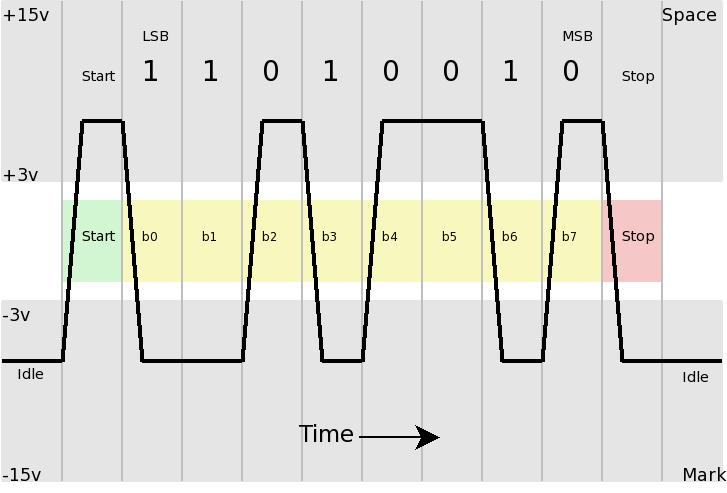
\includegraphics[scale=0.35]{rs232.jpg}
\end{figure}

L'aspetto positivo dell'utilizzo di questo protocollo è la facilità di implementazione di comunicazione: si deve semplicemente impostare la porta seriale e inviare i byte tramite l'apposito registro dell'architettura; l'aspetto negativo è invece la proprietà punto-punto di questa: non possono essere collegati più dispositivi alla stessa porta in invio-ricezione.

Questo protocollo però supporta un dispositivo \textit{spy}, ossia un dispositivo che sta in ascolto su una linea Tx della seriale; in questo modo può leggere i byte inviati da uno dei due dispositivi. Questa informazione si è dimostrata importantissima per l'implementazione del bus.

~

Per far comunicare tutti i dispositivi, è stato creato un bus che permettesse di mantenere le proprietà del protocollo RS232 (quindi comunicazione punto-punto) ma che permettesse anche di far comunicare i dispositivi secondo la logica master-slave di Modbus (quindi ad ogni richiesta del Master deve rispondere lo Slave interrogato). Il bus ha quindi una parte esclusivamente hardware, che consiste nel collegamento fisico tra i dispositivi e un Relè che commuta il canale Tx degli Slave verso il Master, e una parte logica programmata, composta dal microcontrollore PIC16F628A. Questo microcontrollore funge da dispositivo spy, in quanto ha il canale della seriale Rx collegato al canale Tx del Master.

Il funzionamento del bus si basa sulla lettura del primo carattere del messaggio Modbus: il Master invia un messaggio a tutti i dispositivi, il cui primo carattere indica l'indirizzo dello Slave che dovrà rispondere; dal momento che il microcontrollore del bus è un dispositivo spy, ha la possibilità di leggere il primo carattere per ogni messaggio inviato dal Master. Una volta letto il primo carattere, il microcontrollore commuta il canale Tx del bus, in modo che lo Slave abbia accesso esclusivo al canale Rx del Master. In questo modo, tutti ricevono il messaggio Modbus, ma solo chi dovrà rispondere avrà il canale Tx attivato verso il Master.

Per commutare il canale, è stato utilizzato un relè pilotato dal microcontrollore del bus, in base alla lettura del primo carattere del messaggio del Master.

~

Poichè il microcontrollore PIC16F628A non era provvisto di commutatore di segnali RS232 a TTL, è stato aggiunto un MAX222 in modo da trasformare la logica RS232 proveniente dall'esterno in TTL (comprensibile quindi dal microprocessore).

~

~

Per collegarsi a questo bus, è necessario utilizzare un cavo seriale di tipo cross per il dispositivo Master, mentre per i dispositivi Slave serve un cavo dritto.


\begin{figure}[!h]
\centering
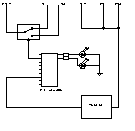
\includegraphics[scale=4.5]{bus.pdf}
\caption{Architettura del bus}
\end{figure}

\newpage
\section{Considerazioni}

È stato deciso di sfruttare tecnologie diverse per far capire come questo sistema possa essere versatile, sfruttando la modularità, e quanti limiti possono esserci utilizzando tecnologie sempre più semplici. Ovviamente si potrebbero prediligere periferiche a basso costo, come nel nostro caso il PIC, però, come si vedrà in seguito, i limiti di progettazione sono talmente vincolanti che è difficile con un singolo PIC gestire tante periferiche quante ne gestisce un Cortex-M3.

~

Sostituire LPC1768 con PIC16F77 sarebbe svantaggioso perché non si avrebbe la stessa potenza di calcolo, quindi servirebbero più PIC e quindi costerebbe relativamente di più, oltrechè non si avrebbero le stesse features. Non si avrebbe nemmeno la stessa versatilità, in quanto se si vuole collegare un nuovo sensore particolare a LPC1768, la riprogrammazione sarebbe molto più veloce e semplice del PIC16F77, quindi porterebbe dei costi maggiori anche a livello di sviluppo software.

~

Se invece il sistema può essere calato in un contesto statico, in cui i cambiamenti di apparecchiature sono molto rare e i sensori che vengono installati sono semplici e pochi, si può pensare di utilizzare un PIC in sostituzione al Cortex-M3.

~

L'unico oggetto che non può essere sostituito con qualcosa di meno costoso è il dispositivo Master, poiché porterebbe a problemi di potenza di calcolo, di rimappatura di tutto il sistema ma soprattutto di costi maggiori di sviluppo software, in quanto il software di questo oggetto è il più complesso di tutto il sistema e di conseguenza riprogettarlo per un'architettura diversa, magari meno potente, porterebbe a dei costi aggiuntivi inutili. 



\section{Altri componenti}

Oltre alla parte operativa del sistema, ci sono vari altri oggetti hardware che devono essere pilotati dai dispositivi slave. Questi sono gli oggetti osservabili del sistema da parte degli utenti e controllano l'ambiente permettendo agli slave di osservare la scena o di illuminarla.

\subsection{Sensori}

I sensori di questo sistema sono di due tipi:

\itema

\item \textbf{attivi}, che hanno una componente hardware/software da alimentare che genera un messaggio o un segnale in base agli avvenimenti che controllano;

\item \textbf{passivi}, che semplicemente generano un segnale in base alle circostanze, senza che debbano essere pilotati da un hardware/software esterno; alcuni non hanno nemmeno bisogno di essere alimentati.

\end{itemize}  

Inoltre possono essere digitali, che generano un segnale digitale per inviare l'analisi al destinatario tramite GPIO, oppure analogici, che generano un segnale analogico che quindi deve essere interpretato tramite ADC dal destinatario.

Questi sensori hanno un costo commerciale molto basso (circa 1 Euro ciascuno) e quindi si adattano benissimo al nostro sistema a basso costo.


Di seguito sono riportati i sensori utilizzati.

~

~


\begin{tabular}{|c  c  c|}
\hline
\multicolumn{1}{|c|}{\textbf {nome}} & \multicolumn{1}{|c|}{\textbf {informazione}} & \multicolumn{1}{c|}{\textbf {funzionamento}} \\
\hline

sensore di umidità e temperatura & Digitale	& attivo  \\
sensore di luminosità		& Digitale	& passivo \\
sensore di distanza		& Digitale	& passivo \\
sensore di rumore		& Digitale	& passivo \\
sensore di distanza ad infrarossi & Digitale	& passivo \\
sensore di vibrazione		& Digitale	& passivo \\

\hline

\textit{\textbf{Totale:}}	& \textbf{6 sensori} & \\

\hline
\end{tabular}

~

~

Poichè questi sensori sono stati saldati su piccole schede elettriche, per rendere possibile l'allacciamento con i dispositivi slave in maniera semplice è stato creato un piccolo circuito per sfruttare facilmente le loro interfacce hardware.
Il circuto, semplificato per tre sensori che mandano il loro messaggio alle rispettive GPIO di uno slave, è il seguente.

~

~

\begin{figure}[!h]
\centering
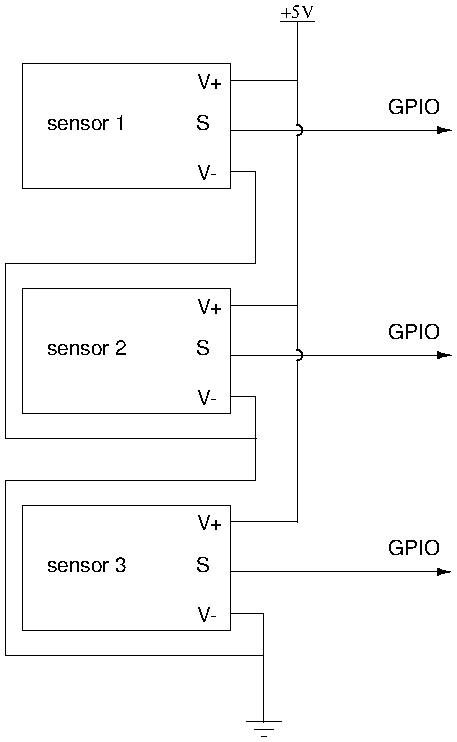
\includegraphics[scale=0.5]{circuitSensor.png}
\end{figure}


~

I sensori offrono diversi controlli per l'ambiente esterno al processore, però la maggior parte di essi restituisce un segnale logico, non un segnale analogico (anche se tutti lo supportano). La scelta del segnale logico è stata imposta da alcune restrizioni della demoboard utilizzata per controllare i sensori: questa demoboard infatti ha il canale ADC occupato da una resistenza variabile, quindi risulta impossibile utilizzare questo canale esternamente.

~

Il comportamento dei sensori è il seguente:

\itema

\item sensore di luminosità: quando si raggiunge la quantità di luce prestabilita, regolabile tramite la resistenza variabile nel circuito, viene inviato un segnale (interpretabile come 1), altrimenti non si invia alcun segnale;

\item sensore di distanza: quando si raggiunge la distanza dal sensore prestabilita, regolabile tramite la resistenza variabile nel circuito, non si invia alcun segnale, altrimenti si invia un segnale interpretabile come ``1'' (ha logica invertita);

\item sensore di rumore: quando si raggiunge una quantità di rumore prestabilita, regolabile tramite la resistenza variabile nel circuito, viene inviato un segnale (interpretabile come 1), altrimenti non si invia alcun segnale;

\item sensore di distanza ad infrarossi: quando si raggiunge la distanza dal sensore prestabilita, regolabile tramite le due resistenze, una per la sensibilità di controllo infrarosso e l'altra per la frequenza dell'infrarosso emesso, non si invia alcun segnale, altrimenti si invia un segnale interpretabile come ``1'' (ha logica invertita);

\item sensore di vibrazione: quando viene scosso il sensore, quindi quando la molla interna al sensore crea un contatto con la parete di questo chiudendo il circuito, viene inviato un segnale (interpretabile come 1), altrimenti non si invia alcun segnale.

\end{itemize} 


Per un corretto funzionamento di questi sensori, è necessario collegare la massa dei sensori con quella delle GPIO che li andranno a pilotare, altrimenti non funzioneranno.

\subsection{DHT11}

Il sensore temperatura e umidità DHT11 merita particolare attenzione, in quanto utilizza un protocollo di comunicazione standard particolare nonostante sia un sensore piccolo e a basso costo. Questo sensore è in grado di comunicare i dati acquisiti (con aggiornamento di 1 Hz) tramite protocollo \textit{1-Wire}, comunicando in 4 millisecondi il risultato. Per collegare il sensore all'unità di controllo, è necessario realizzare questo piccolo circuito:

\begin{figure}[!h]
\centering
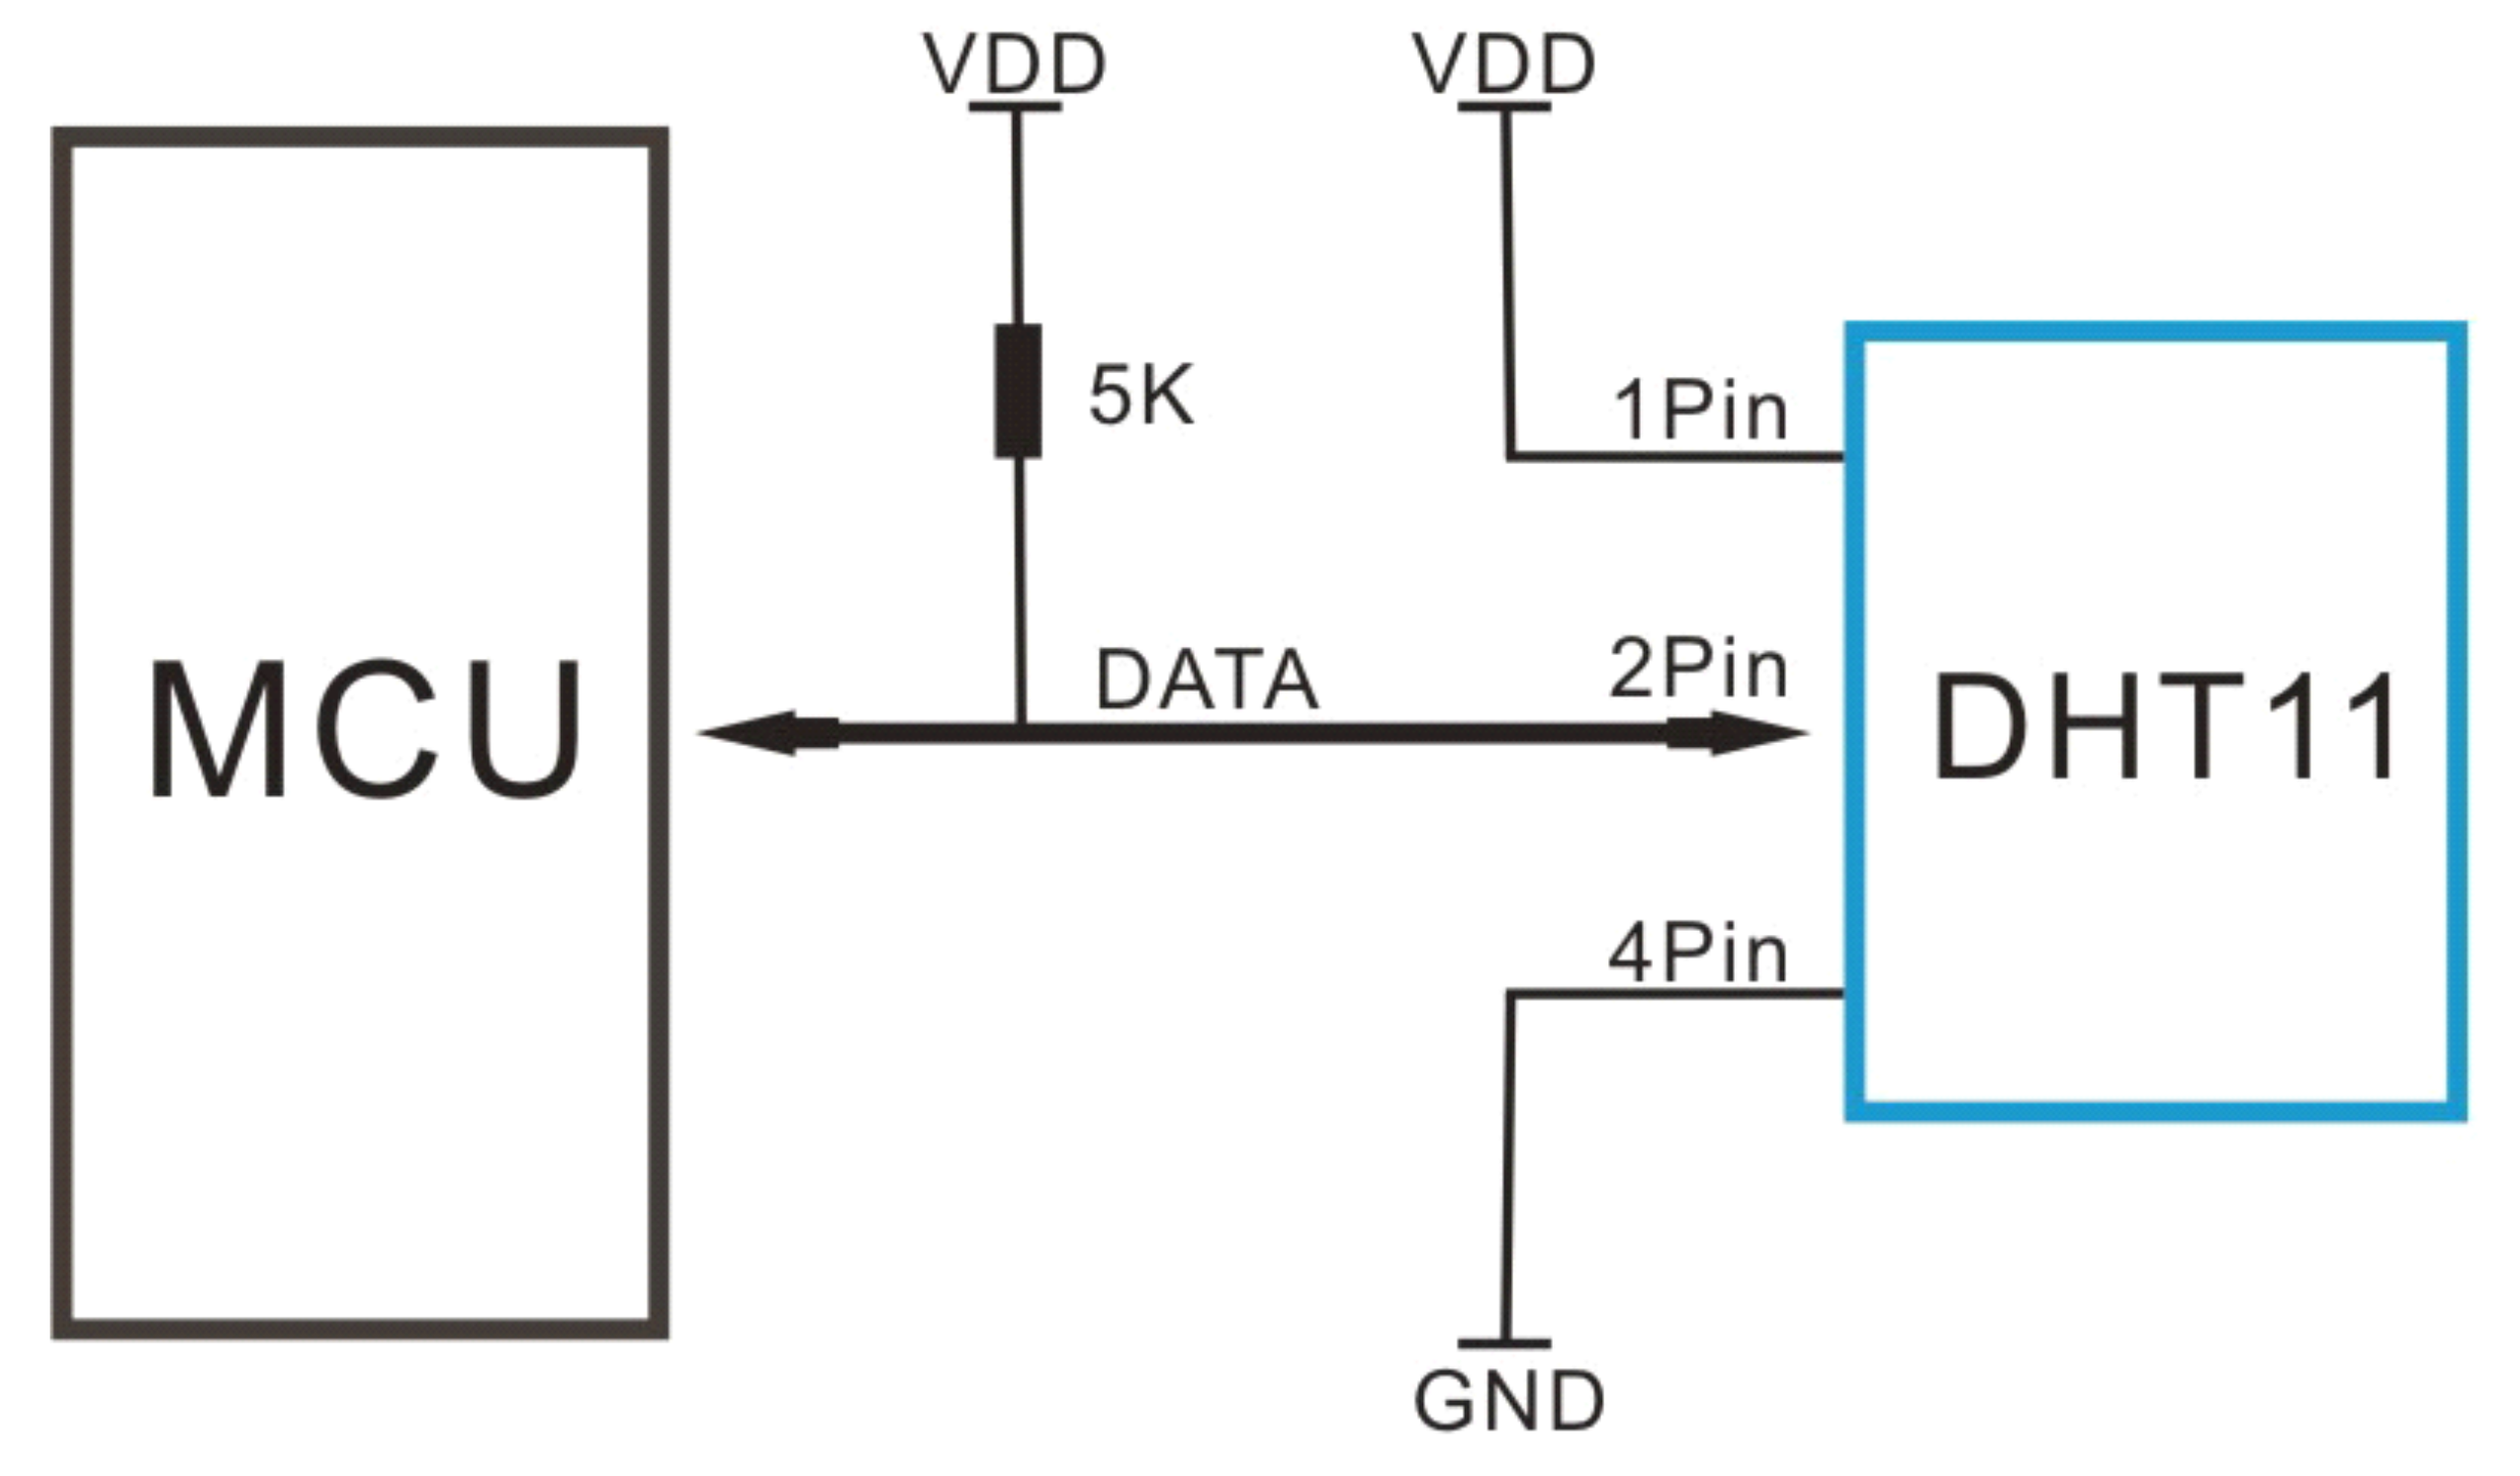
\includegraphics[scale=0.6]{DHT11_collegamento.png}
\end{figure}


La particolarità del protocollo 1-Wire è la semplicità di implementazione e la capacità di non richiedere un hardware specifico (infatti il protocollo è stato implementato utilizzando una GPIO del processore LPC1768). Il funzionamento è il seguente: 

\begin{enumerate}

\item si esegue un ack, ossia il microprocessore invia un segnale logico basso per 20 millisecondi e alto per 40 microsecondi, il sensore risponde con un segnale basso di 80 microsecondi e alto per 40 microsecondi;

\item il sensore invia il dato, ossia invia un segnale basso per almeno 40 microsecondi, poi alto per un tempo variabile di microsecondi: se il segnale dura più di 30 microsecondi, il segnale deve essere interpretato come ``1'', altrimenti come ``0''.

\end{enumerate}

~

\begin{figure}[!h]
\centering
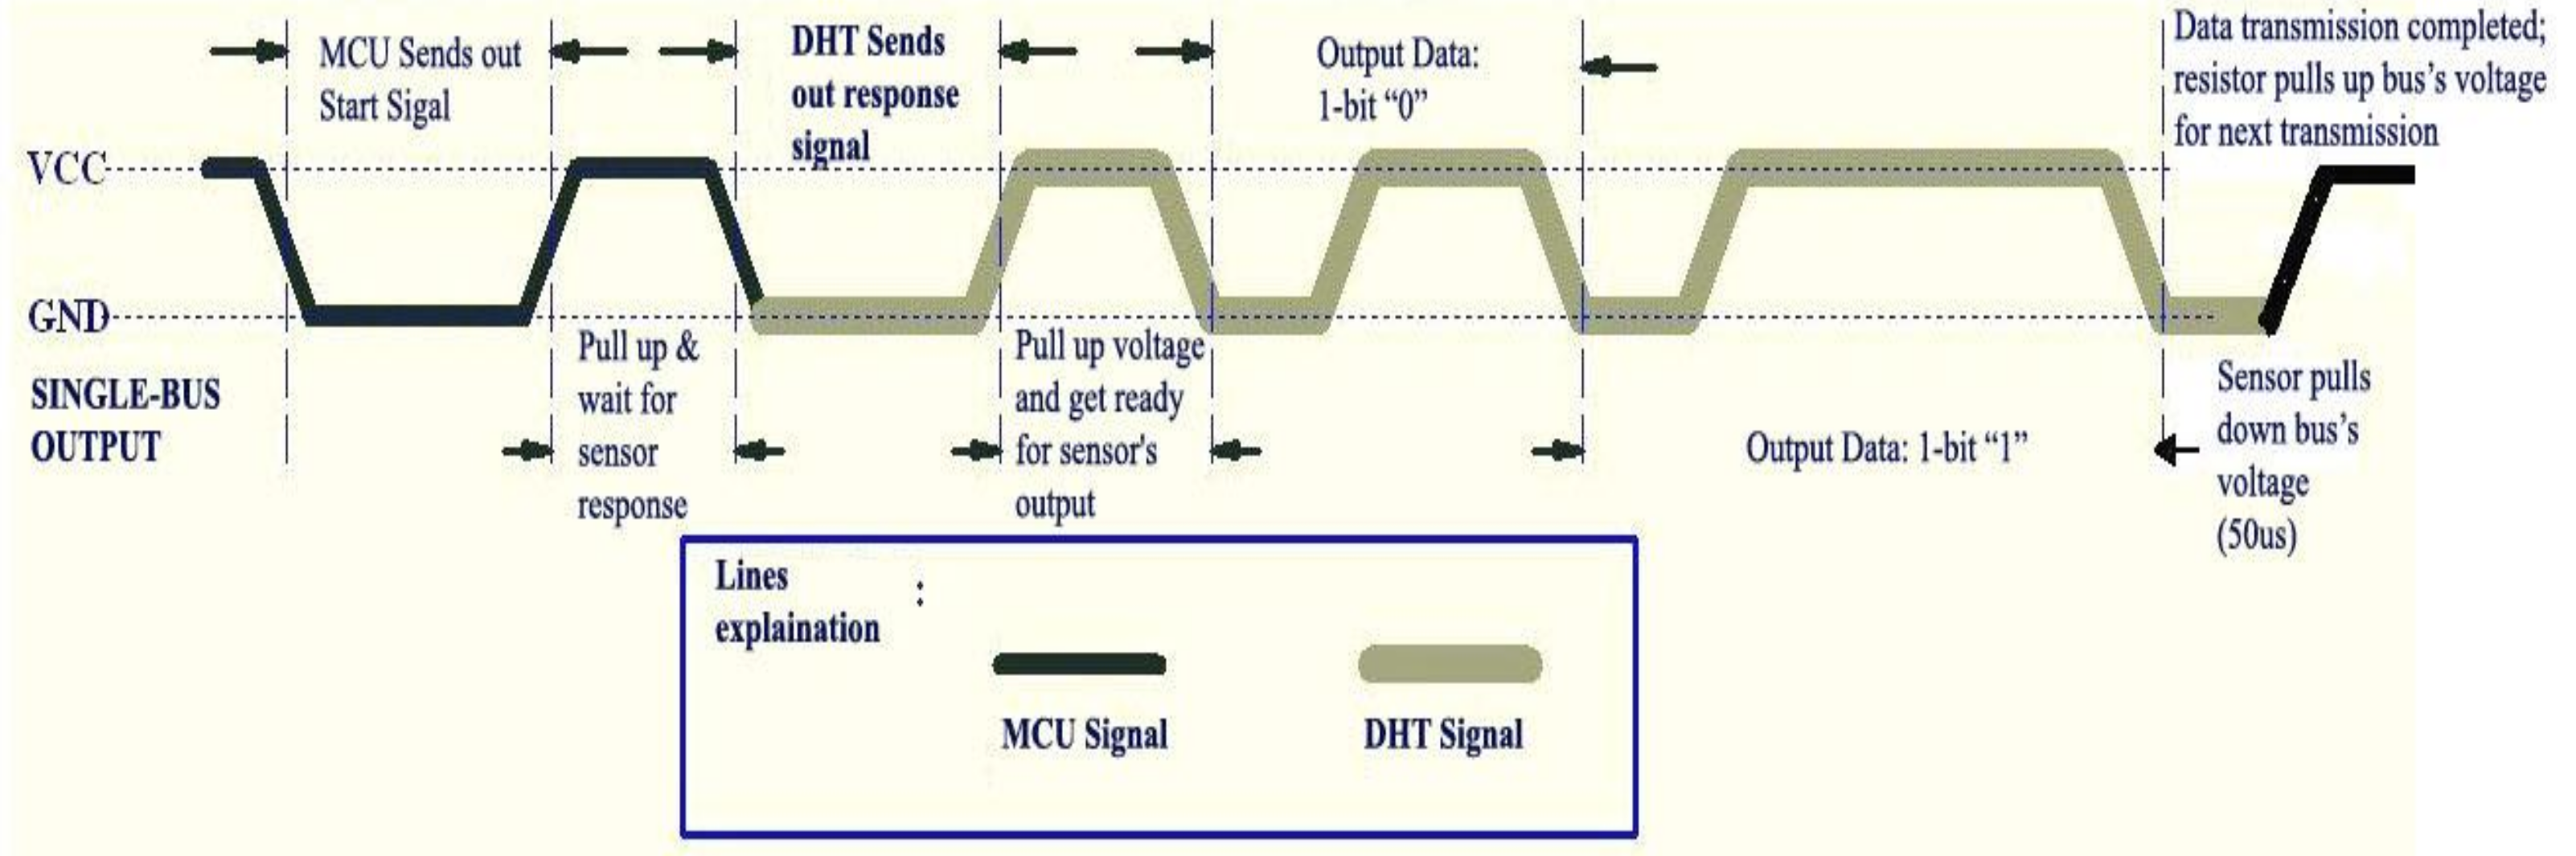
\includegraphics[scale=1]{1wire.png}
\end{figure}

~

Questo sensore invia in totale 40 segnali, che corrisponderanno a 40 bit: 8 per l'umidità, 8 per la parte decimale dell'umidità, 8 per la temperatura, 8 per la parte decimale della temperatura, 8 per il CRC, che dovrebbe corrispondere alla somma dei numeri precedenti rappresentati dagli 8 bit interpretati in modulo.

~

L'aspetto positivo dell'utilizzo di questo sensore è la semplicità di implementazione del protocollo, oltrechè l'utilizzo di una GPIO piuttosto che l'utilizzo di un'ingresso ADC; questo aspetto è da considerare ottimo quando l'architettura utilizzata non dispone di un convertitore analogico-digitale. L'utilizzo di questo sensore ha anche diversi aspetti negativi:

\itema

\item nonostante la comunicazione duri 4 ms, occupa completamente l'utilizzo del processore, poiché questo deve contare per quandi microsecondi il sensore invia i segnali, quindi un calcolo molto oneroso in quanto 1 microsecondo corrisponde a 1 MHz;

\item pur avendo il controllo CRC, la comunicazione molto spesso non funziona; infatti essendoci anche il minimo disturbo durante la comunicazione, dovuto sia da aspetti software (un task asincrono che viene schedulato può essere interpretato come disturbo in questo caso) che hardware (disturbi o ossido nei contatti), il segnale ricevuto risulta corrotto e quindi è necessario richiedere nuovamente la misurazione. 

\end{itemize}

Questi due aspetti sono stati molto importanti durante la progettazione in quanto si è cercato di ottimizzare al massimo l'utilizzo del processore incaricato di leggere la temperatura, eliminando tutti i possibili disturbi software e hardware.

\subsection{Relè}

Poichè sarà necessario pilotare anche luci di abitazioni, gli slave non possono essere in grado di erogare abbastanza corrente per queste. Per risolvere questo problema, è necessario utilizzare un componente hardware chiamato Relè. Questo oggetto consiste in un avvolgimento di rame e una lamina di rame che funge da switch di canale; appena l'avvolgimento viene eccitato con la corrente, genera un campo magnetico che sposta la lamina di rame in modo da deviare la corrente da un canale all'altro. Anche la bobina di rame però necessita di molta corrente per generare un campo magnetico; è presente quindi un fotocopiatore che riceve in input sia la corrente necessaria alla bobina per generare il campo magnetico sia la corrente dello slave per pilotare via software le luci; in output invierà la corrente necessaria per il relé solo quando lo slave invia il segnale.

Questo oggetto può quindi essere utilizzato come interruttore automatico pilotato dal processore. È stata utilizzata una scheda per pilotare 8 relè tramite le GPIO di uno slave, in modo da accendere o spegnere le luci a led a basso consumo.

~

Per un corretto funzionamento, è necessario collegare la massa di questo circuito alla massa del processore che lo deve pilotare, altrimenti non funzionerà l'invio del segnale.

\subsection{Luci a led}

È stato deciso di pilotare delle luci a led tramite i Relè per dimostrare un'ulteriore applicazione di questo progetto, ossia l'illuminazione della casa automatizzata. Per non utilizzare troppo spazio e non consumare troppa corrente, è stato deciso di utilizzare delle strip led da arredamento a basso consumo. 

\subsection{Foto del sistema hardware}

\begin{figure}[!h]
\centering
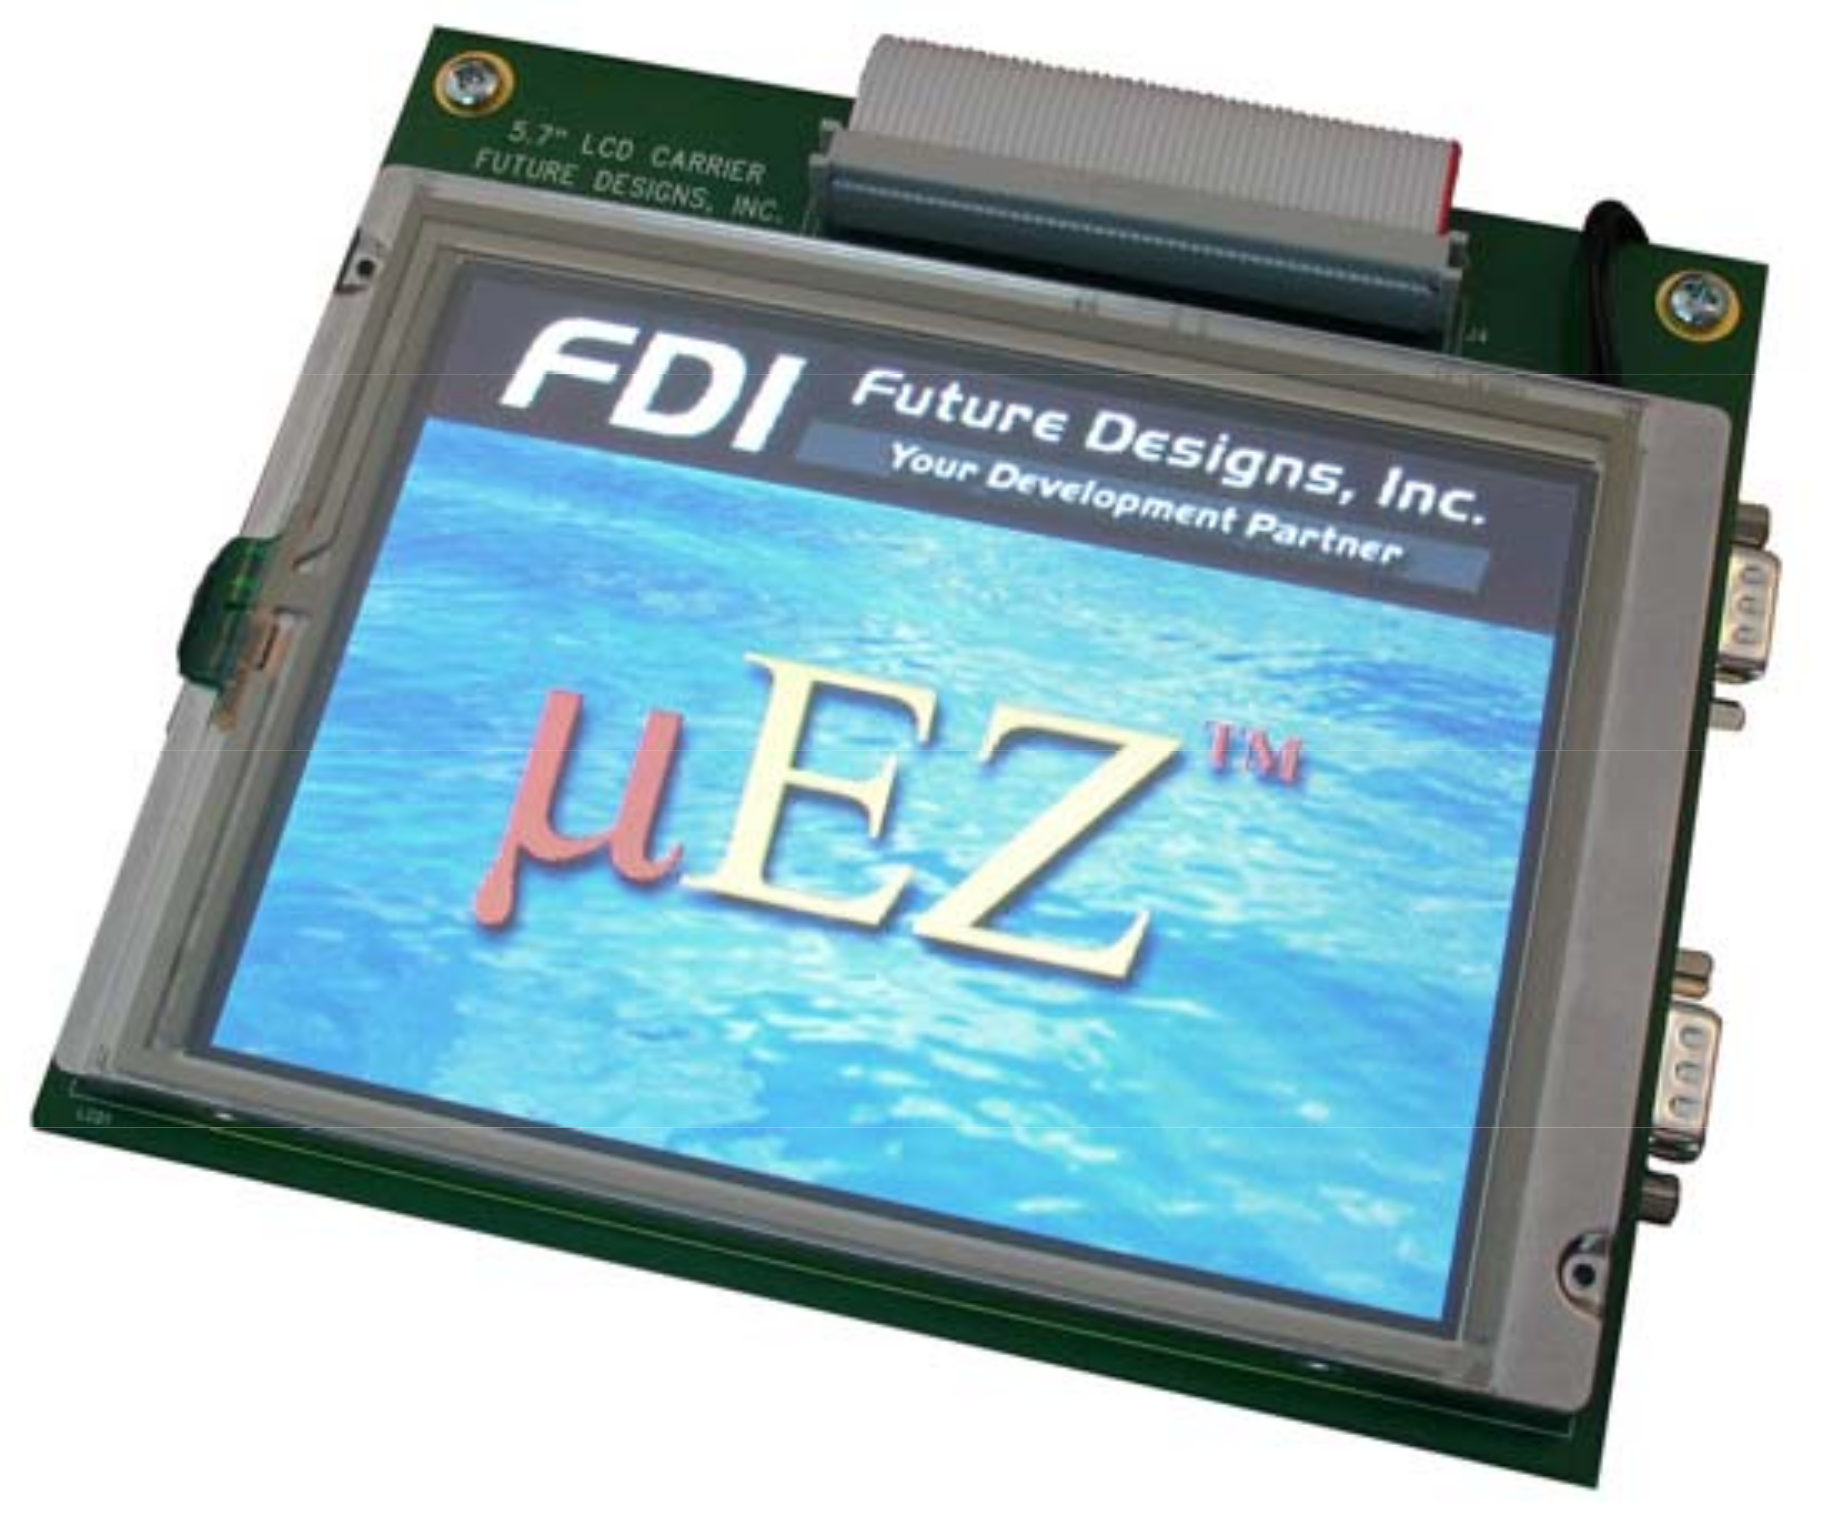
\includegraphics[scale=1]{lpc1788.png}
\caption{LPC1788}
\end{figure}


\begin{figure}[!h]
\centering
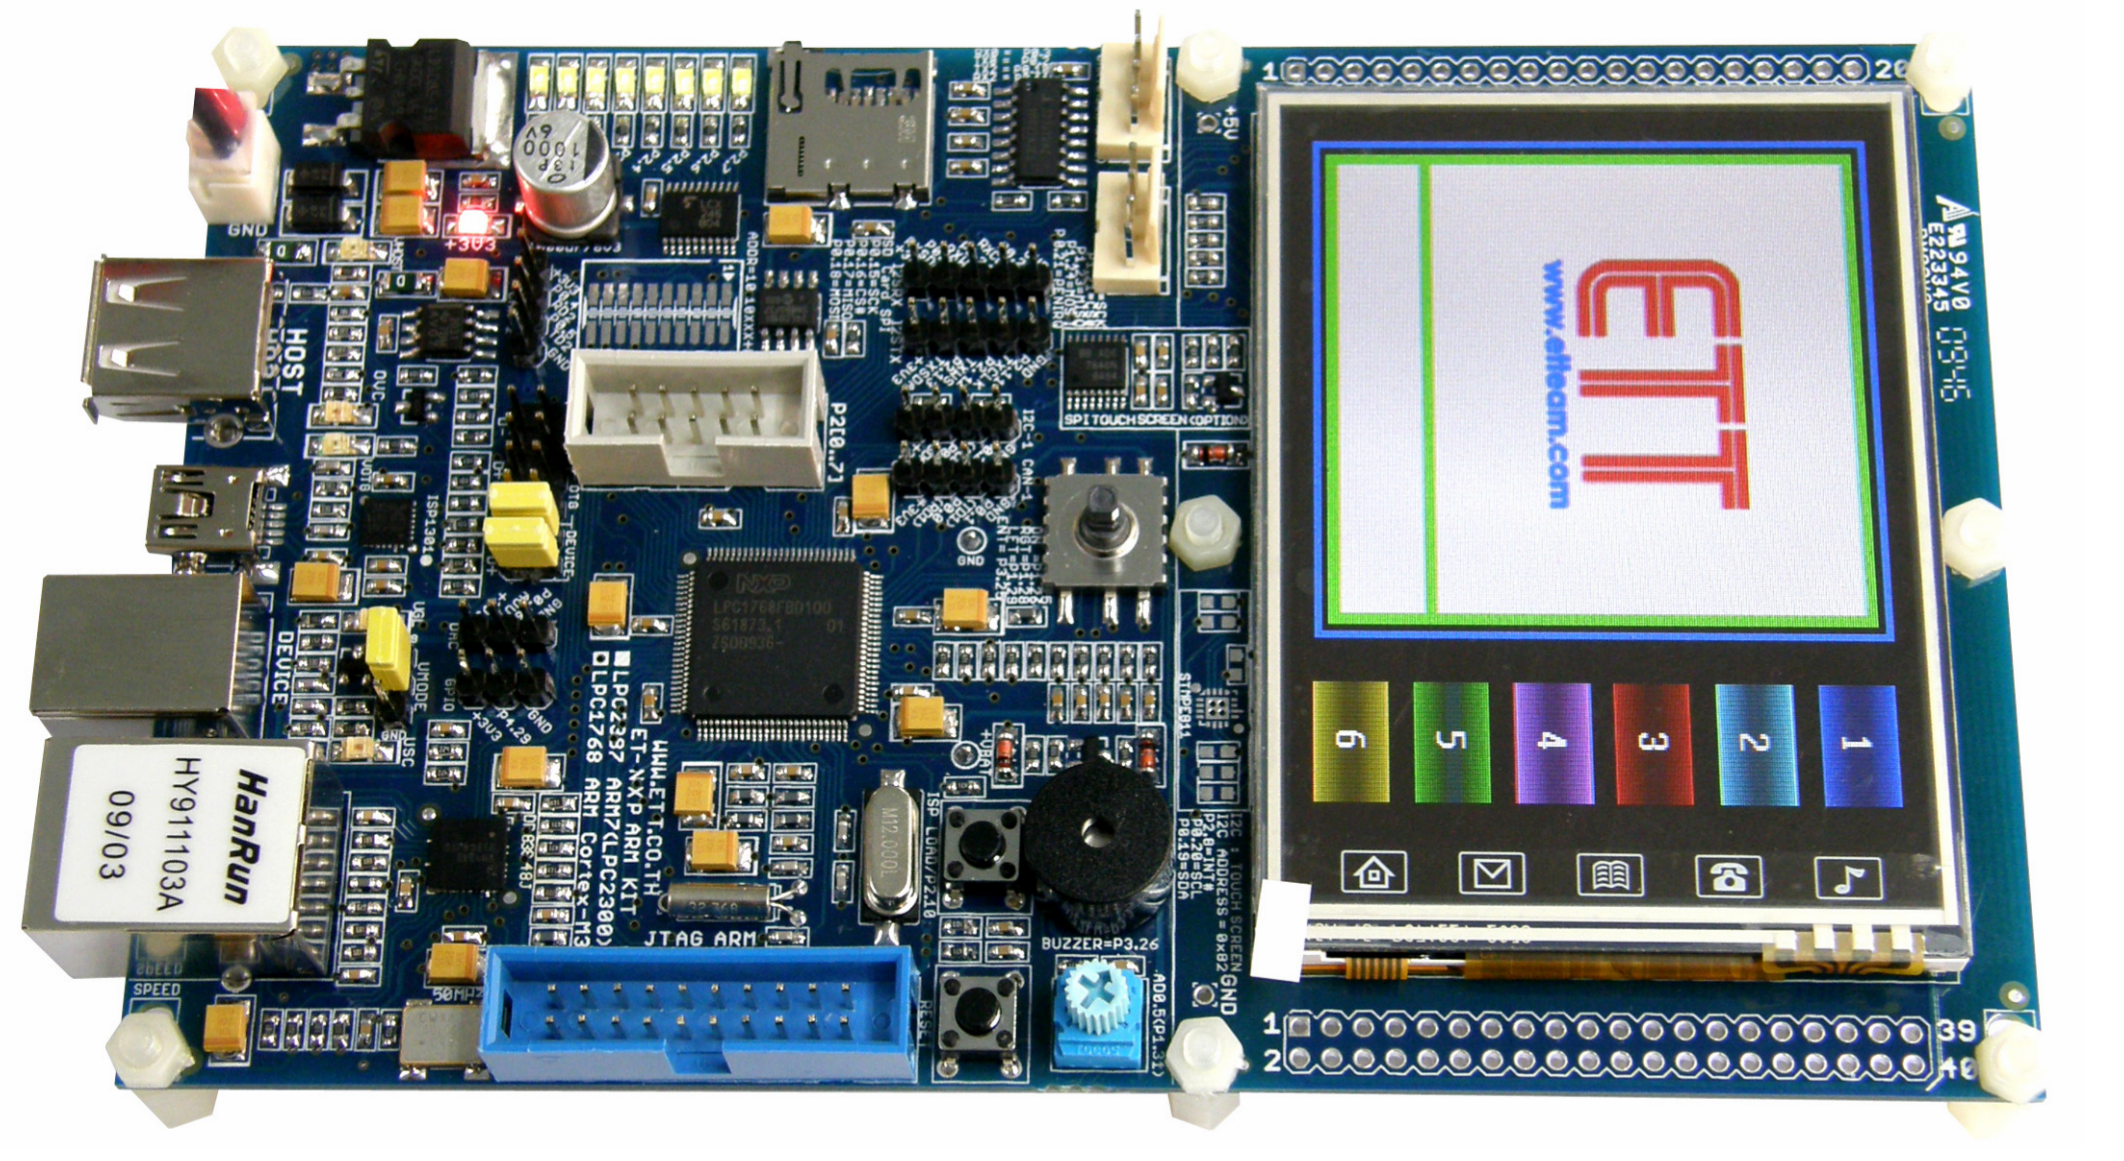
\includegraphics[scale=1]{lpc1768.png}
\caption{LPC1768}
\end{figure}


\begin{figure}[!h]
\centering
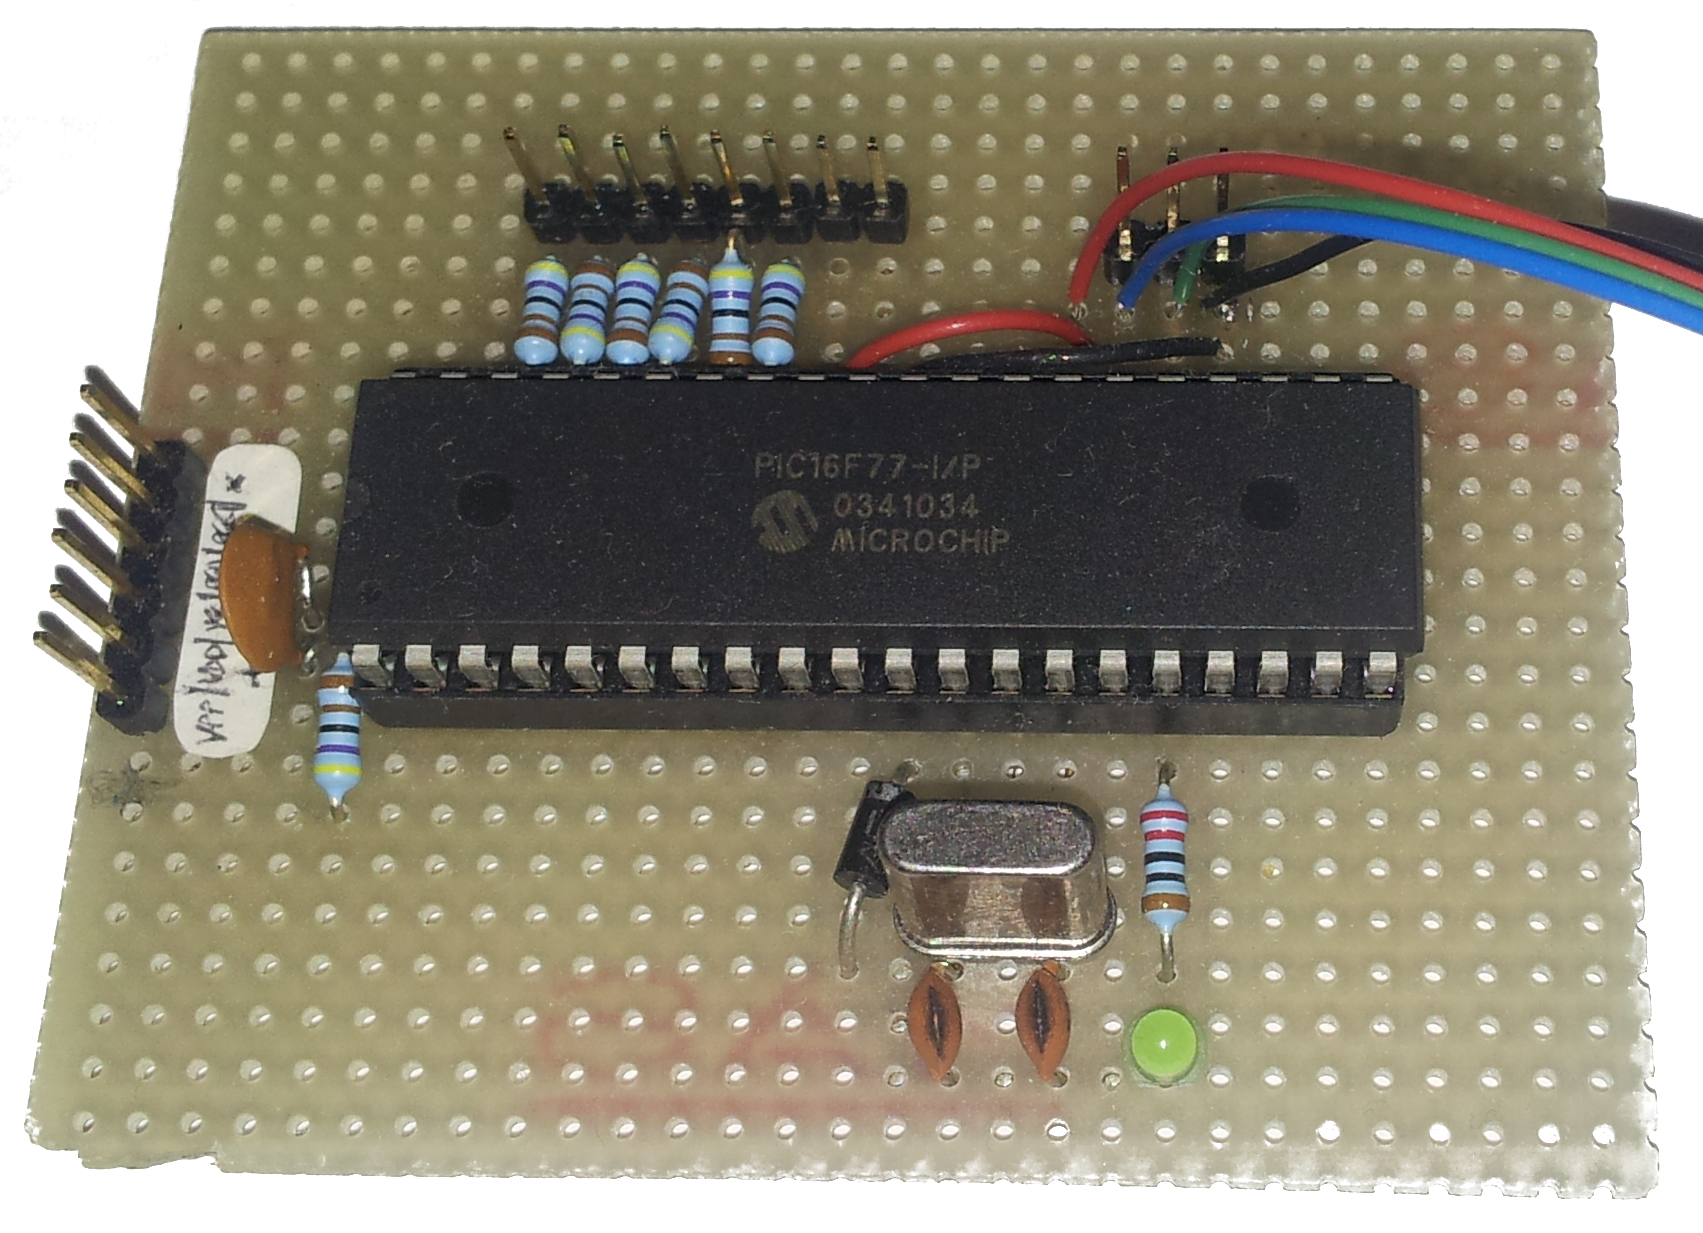
\includegraphics[scale=0.15]{pic16f77.png}
\caption{PIC16F77}
\end{figure}

\begin{figure}[!h]
\centering
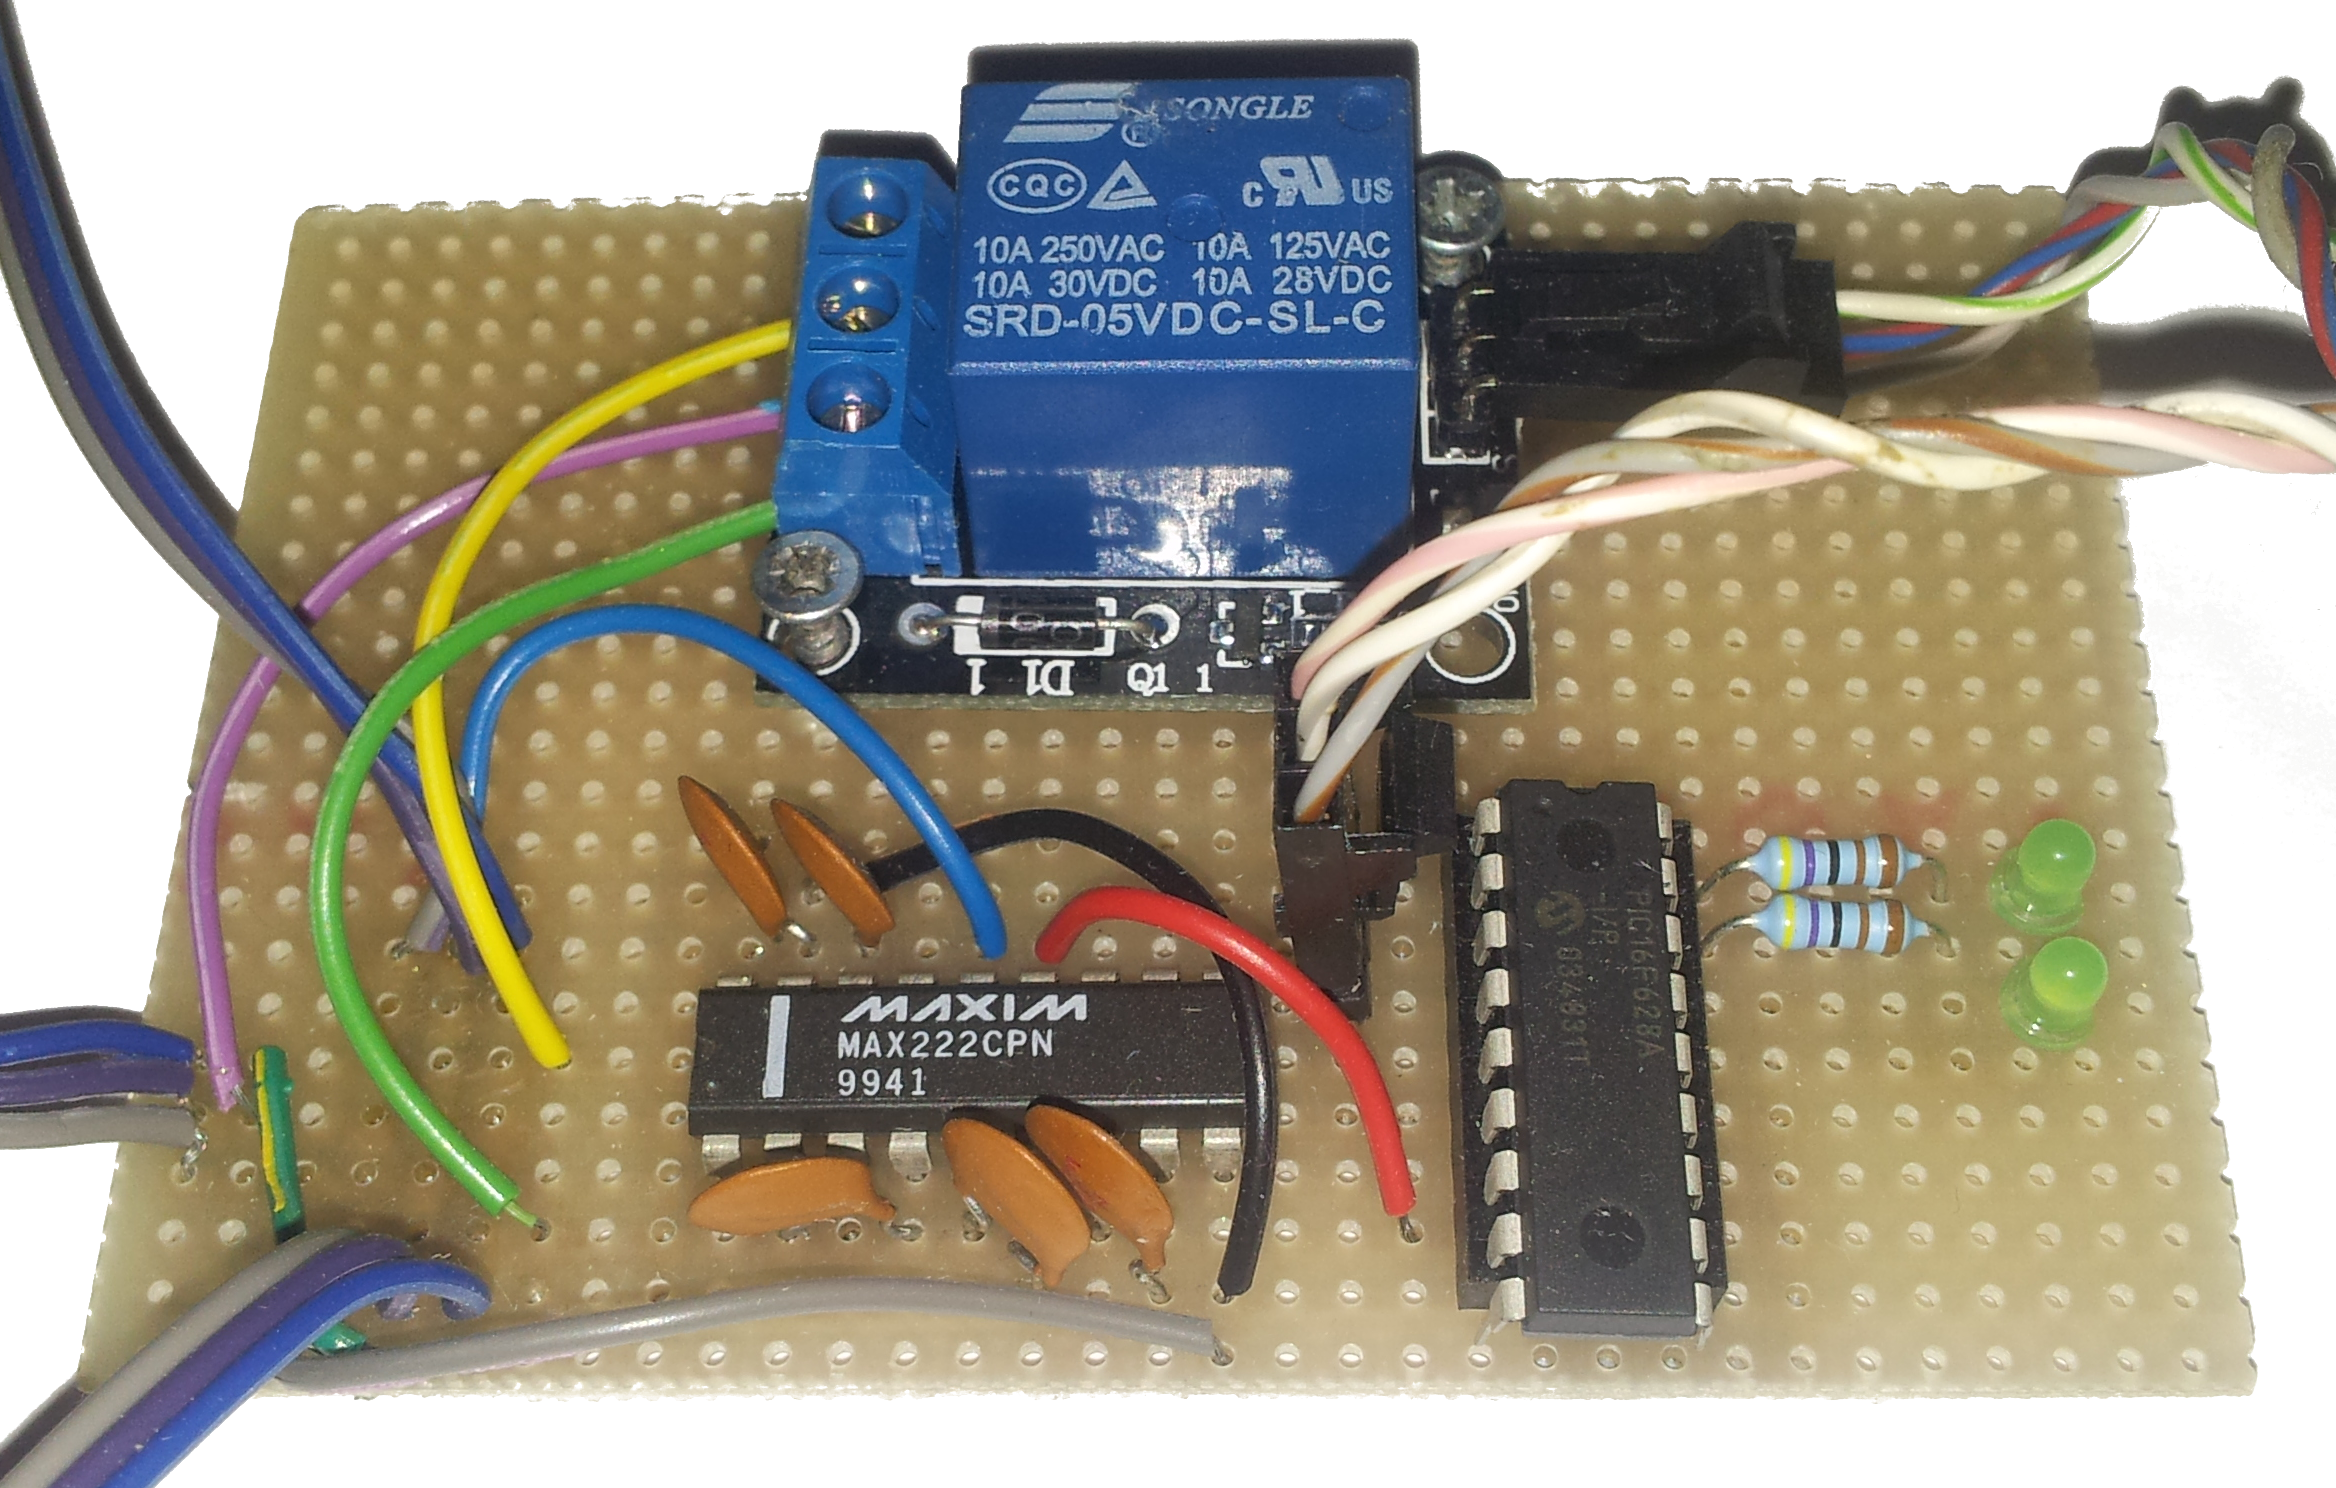
\includegraphics[scale=0.12]{bus_foto.png}
\caption{BUS RS232}
\end{figure}

\begin{figure}[!h]
\centering
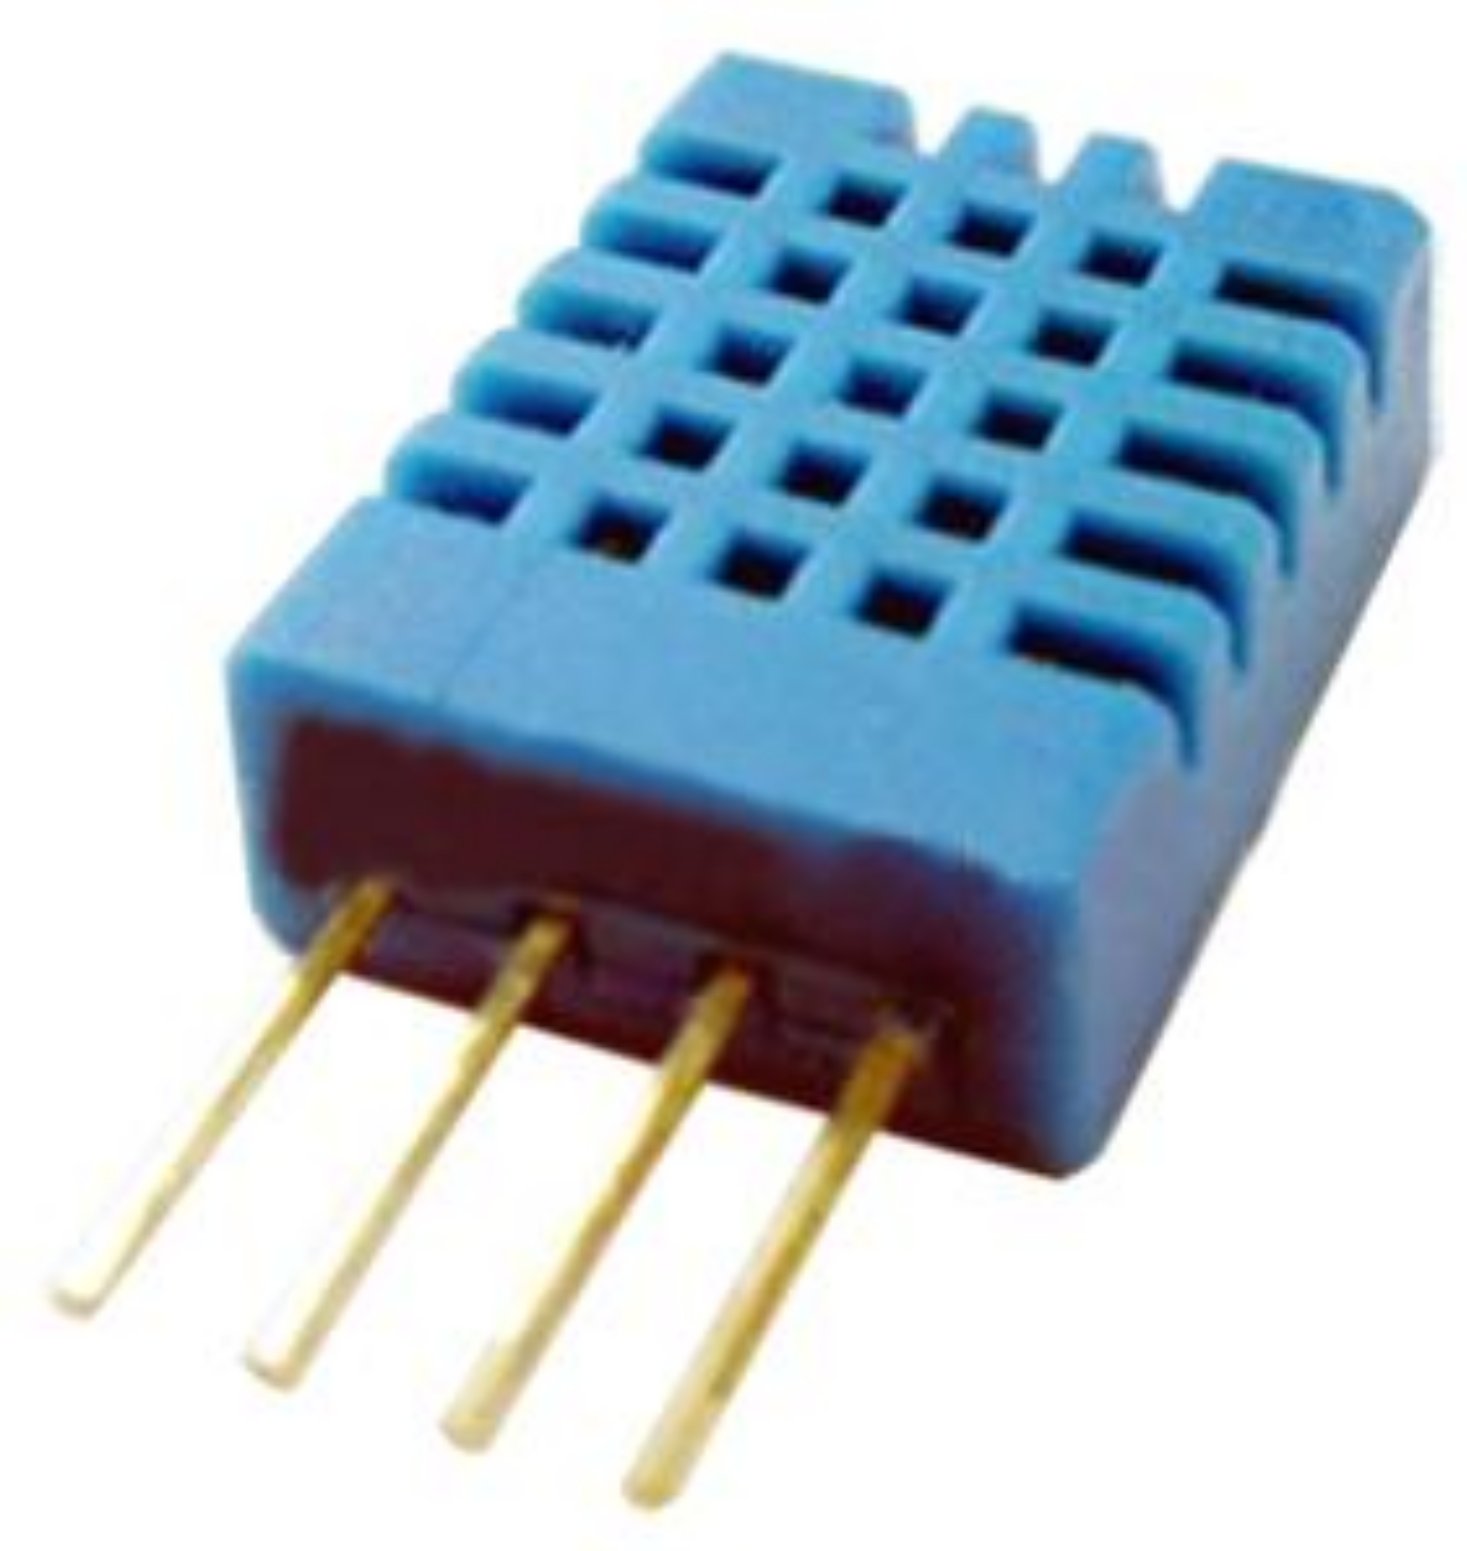
\includegraphics[scale=0.5]{DHT11.png}
\caption{Sensore DHT11}
\end{figure}


\begin{figure}[!h]
\centering
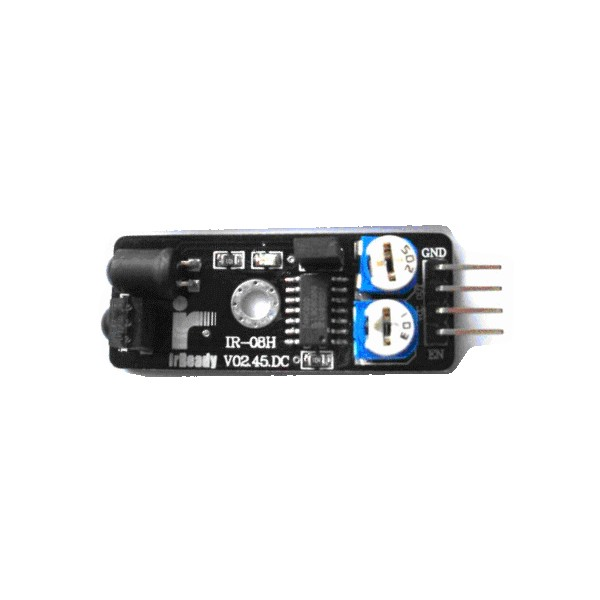
\includegraphics[scale=0.5]{dist1.jpg}
\caption{Sensore di distanza a infrarossi}
\end{figure}


\begin{figure}[!h]
\centering
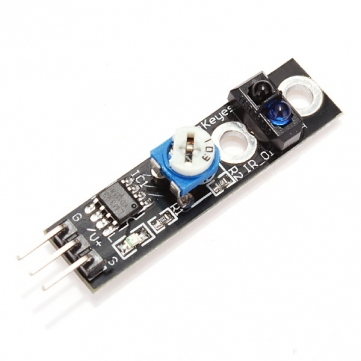
\includegraphics[scale=0.5]{dist2.jpg}
\caption{Sensore di distanza}
\end{figure}


\begin{figure}[!h]
\centering
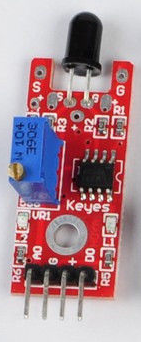
\includegraphics[scale=0.6]{lumi.png}
\caption{Sensore luminosità}
\end{figure}


\begin{figure}[!h]
\centering
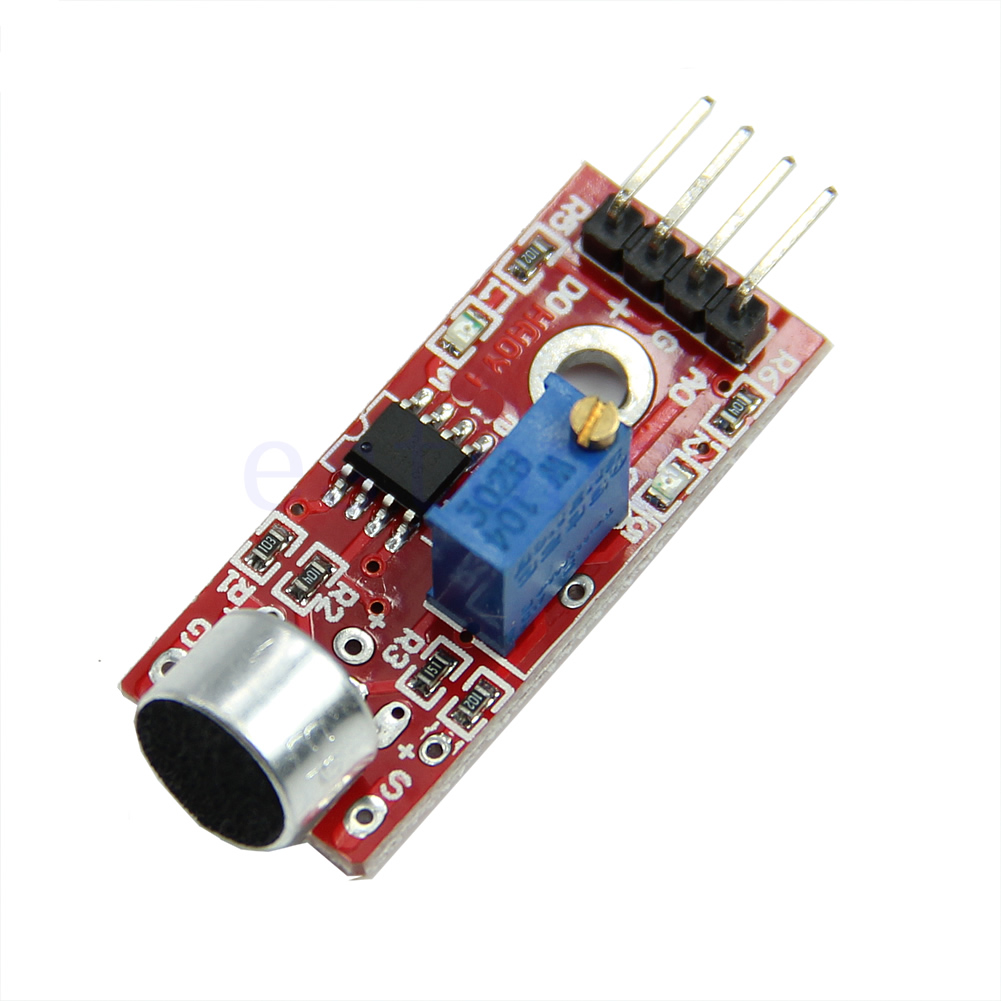
\includegraphics[scale=0.2]{mic.jpg}
\caption{Sensore di rumore}
\end{figure}


\begin{figure}[!h]
\centering
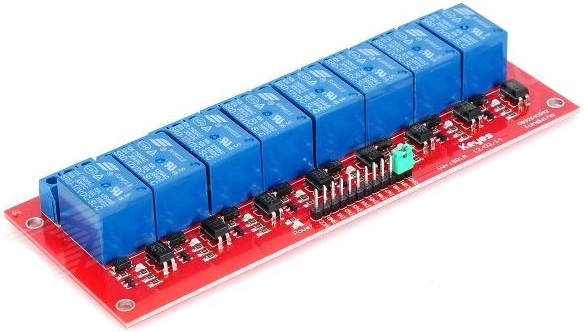
\includegraphics[scale=0.5]{rele.jpg}
\caption{8 relè}
\end{figure}

\begin{figure}[!h]
\centering
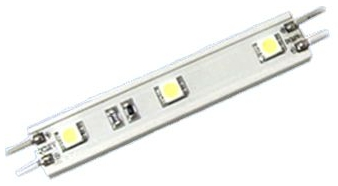
\includegraphics[scale=0.5]{led.jpg}
\caption{Strip led}
\end{figure}


%%%%%%%%%%%%%%%%%%%%%%%%%%%%%%%%%%%%%%%%%%%%%%%%%%%%%%%%%%%%%%%%%%%%%%%%%%%%%%%%%%%%%%%%%%%%%%%%%%%%%%%%%%%%%%%%%%%%%%%%%%%%%%%%%%%%%%%%%
%%%%%%%%%%%%%%%%%%%%%%%%%%%%%%%%%%%%%%%%%%%%%%%%%%%%%%%%%%%%%%%%%%%%%%%%%%%%%%%%%%%%%%%%%%%%%%%%%%%%%%%%%%%%%%%%%%%%%%%%%%%%%%%%%%%%%%%%%
%%%%%%%%%%%%%%%%%%%%%%%%%%%%%%%%%%%%%%%%%%%%%%%%%%%%%%%%%%%%%%%%%%%%%%%%%%%%%%%%%%%%%%%%%%%%%%%%%%%%%%%%%%%%%%%%%%%%%%%%%%%%%%%%%%%%%%%%%
%%%%%%%%%%%%%%%%%%%%%%%%%%%%%%%%%%%%%%%%%%%%%%%%%%%%%%%%%%%%%%%%%%%%%%%%%%%%%%%%%%%%%%%%%%%%%%%%%%%%%%%%%%%%%%%%%%%%%%%%%%%%%%%%%%%%%%%%%


\chapter{Architettura Software}

La parte più interessante di questo preambolo al progetto realizzato è lo scheletro software su cui si basa tutta la progettazione. È facile pensare alla programmazione in un ambiente in cui il sistema operativo offre un ``\textit{hardware abstraction layer}'' che garantisce una facile programmazione. Nell'ambito però dei sistemi embedded, un HAL è pressochè assente, quindi la programmazione si complica in quanto bisogna ragionare sul funzionamento dell'architettura stessa.


\section{Dispositivo Master}

Per LPC1788 il problema principale era quello di gestire l'interfaccia grafica e l'invio di messaggi agli Slave. Per gestire facilmente ciò, è stato utilizzato un sistema preconfezionato che offre delle API utili alla gestione di periferiche e per la progettazione. 


\subsection{uEZ}
Questo sistema si chiama $\mu EZ$, chiamato così perché dovrebbe ``ispirare'' il designer di software embedded durante la progettazione e semplificarla. Sono state comunque modificate delle API per semplificare l'utilizzo della porta seriale e dei timer.

~

\begin{figure}[!h]
\centering
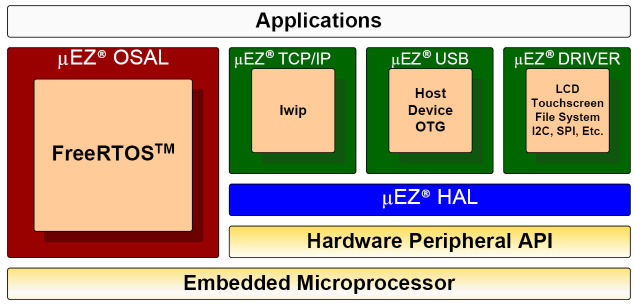
\includegraphics[scale=0.7]{uEZ.png}
\caption{architettura del sistema uEZ}
\end{figure}

Il sistema offre innanzitutto un HAL completa, in quanto permette di trattare ad alto livello la configurazione di tutte le periferiche. Inoltre non è necessario definire il boot di sistema (cosa non banale per questi sistemi). Esiste un porting standard per ogni processore, se non è presente è possibile scriverlo facilmente. Il sistema deve essere compilato in due passaggi: il primo consiste nel compilare $\mu EZ$ per la propria architettura, ottenendo un file di libreria da linkare al proprio progetto, il secondo consiste nello sviluppare il proprio progetto basandosi su questo sistema. È possibile, al tempo di compilazione, decidere quali periferiche utilizzare prima di generare la libreria da linkare, ottimizzando per area il proprio software.

~

Ciò che ha portato allo sviluppo su questo sistema software è stato, oltre all'astrazione dell'hardware che facilita la programmazione, alla predisposizione da parte del sistema di usare risorse di rete come lo stack di rete lwIP e alla presenza di sistema operativo FreeRTOS, è stata la capacità di utilizzare una libreria grafica per i sistemi embedded, ossia la libreria \textbf{emWIN}.

\subsection{emWin}

Questa è una libreria grafica per sistemi embedded basata su una grafica molto simile alle prime versioni di Windows (sia per l'estetica sia per la gestione ottimale delle risorse grafiche). Essa offre un HAL ad alto livello molto semplice da utilizzare, con cui è possibile progettare interfacce con oggetti grafici ben noti (bottoni, input text, ecc...) senza dover interfacciarsi direttamente con l'oggetto hardware. Può sembrare una soluzione poco ottimale, visto che tutti gli elementi ad ``alto livello'' nella progettazione di sistemi embedded può essere reputata poco efficiente in ambito di risorse e computazione, in realtà è stata progettata in maniera altamente ottimizzata.

La gestione dell'interfaccia tramite questa libreria ha un'implementazione molto semplice:

\begin{enumerate}[noitemsep,topsep=18pt,parsep=10pt,partopsep=0pt]
\item si descrive l'interfaccia implementandola personalmente o tramite appositi programmi di generazione di codice (GUIBuilder incluso nel pacchetto emWin);
\item si associa al codice corrente l'intefaccia appena creata ricordandosi di usare il comando \\\lstinline!ExecDialogBox()! (vedere manuale emWin);
\item si associa ai widget creati il codice che viene eseguito in base agli eventi generati.

\end{enumerate}



Il porting che è stato fatto di questa libreria per questo processore dipende dalla board di sviluppo che si vuole considerare (soprattutto per il nostro LCD TouchScreen), nel nostro caso dipende in maniera esclusiva da $\mu EZ$. Infatti per questioni di modularità, emWin si appoggia alle API di $\mu EZ$, in modo da sfruttarle senza interfacciarsi direttamente con l'hardware sottostante , essendo già state ottimizzate le API di $\mu EZ$ (quindi emWin nel nostro caso non può funzionare senza di $\mu EZ$).
 
\section{Dispositivi Slave}

Questi dispositivi non hanno una parte software che funge da scheletro per l'applicazione, essenzialmente per due motivi:

\itema

\item le architetture sono troppo semplici, non è necessario interfacciarsi con l'hardware tramite API visto che i comandi che devono eseguire sono diretti alle diverse periferiche;
\item non è presente molta memoria e non è garantita molta capacità di calcolo, quindi sarebbe svantaggioso utilizzare qualcosa di più ``astratto'' (e quindi inefficiente) per gestire le operazioni.

\end{itemize}

L'unica eccezione di questo argomento è l'utilizzo, per il dispositivo ARM, di un sistema operativo. Per il dispositivo PIC non è stato possibile inserire il sistema operativo, in quanto non è presente abbastanza memoria e il sistema di calcolo è troppo semplice.

\subsection{FreeRTOS}

Il sistema operativo utilizzato sul dispositivo di tipo ARM Cortex-M3 si chiama FreeRTOS. 

È un sistema operativo di tipo Real Time, ossia  il sistema deve essere ``prevedibile'' o piuttosto ``determinista'', nel senso che nel sistema si deve conoscere la tempistica reale (nei migliori o peggiori dei casi) di un determinato processo o elaborazione. In pratica un sistema real-time deve garantire che una elaborazione (o task) termini entro un dato vincolo temporale o scadenza (detta in gergo deadline). Per garantire questo è richiesto che la schedulazione delle operazioni sia fattibile. Il concetto di fattibilità di schedulazione è alla base della teoria dei sistemi real-time ed è quello che ci permette di dire se un insieme di task sia eseguibile o meno in funzione dei vincoli temporali dati.

Il sistema operativo non è stato utilizzato per utilizzare una HAL per programmare, ma per creare dei task separati per gestire la parte di protocollo e la parte di applicazione, in quanto continui polling sui sensori possono disturbare l'invio della risposta al dispositivo Master. Alla fine della progettazione però, per i vincoli dettati dal sensore DHT11, si è deciso di creare un unico task che permettesse di sfruttare la velocità di FreeRTOS nell'esecuzione di un task.



%%%%%%%%%%%%%%%%%%%%%%%%%%%%%%%%%%%%%%%%%%%%%%%%%%%%%%%%%%%%%%%%%%%%%%%%%%%%%%%%%%%%%%%%%%%%%%%%%%%%%%%%%%%%%%%%%%%%%%%%%%%%%%%%%%%%%%%%%
%%%%%%%%%%%%%%%%%%%%%%%%%%%%%%%%%%%%%%%%%%%%%%%%%%%%%%%%%%%%%%%%%%%%%%%%%%%%%%%%%%%%%%%%%%%%%%%%%%%%%%%%%%%%%%%%%%%%%%%%%%%%%%%%%%%%%%%%%
%%%%%%%%%%%%%%%%%%%%%%%%%%%%%%%%%%%%%%%%%%%%%%%%%%%%%%%%%%%%%%%%%%%%%%%%%%%%%%%%%%%%%%%%%%%%%%%%%%%%%%%%%%%%%%%%%%%%%%%%%%%%%%%%%%%%%%%%%
%%%%%%%%%%%%%%%%%%%%%%%%%%%%%%%%%%%%%%%%%%%%%%%%%%%%%%%%%%%%%%%%%%%%%%%%%%%%%%%%%%%%%%%%%%%%%%%%%%%%%%%%%%%%%%%%%%%%%%%%%%%%%%%%%%%%%%%%%

\chapter{Modello di sistema}

Di seguito si riporta il modello del sistema secondo lo standard ingegneristico, ossia presentando:

\itema 

\item\textit{``Use Case Diagram''}, ossia la presentazione ad alto livello dei diversi attori del sistema (nel nostro caso gli attori sono: l'utente, il dispositivo Master e il dispositivo Slave), in modo da rendere chiari i ruoli degli attori e le loro azioni all'interno dello scenario;
\item\textit{``Sequence Diagram''}, ossia la presentazione ad alto livello dello scambio di ``messaggi'' tra i diversi attori e dispositivi del sistema (vengono identificate le interazioni nel sistema come messaggi).

\end{itemize}

È stato deciso di ingegnerizzare questo progetto in quanto le risorse disponibili erano troppo poche per permettere errori di valutazione, oltrechè si voleva creare un progetto mantenibile nel tempo, quindi era necessaria una documentazione appropriata.

\section{Use Case Diagram}

Con questo tipo di diagramma, viene presentata una tabella per ogni attore, ciascuna contenente nell'intestazione il nome dell'attore considerato e all'interno le rispettive azioni. Ogni attore coinvolto nel sistema ha delle precondizioni da rispettare affinchè tutte le operazioni vadano a buon fine e una postcondizione. Vengono presentate infine le azioni sotto forma di algoritmo o insieme di attività da svolgere per eseguire un task.

L'attore principale, cioè l'utente, ha tre tipi di attività, ossia la scelta del task da far eseguire al sistema, l'avvio di esecuzione di tale task (premendo l'opportuno tasto nell'interfaccia) e l'osservazione dei valori che vengono mostrati nella GUI.

L'altro attore è il dispositivo Master, che ha il compito di mostrare ed aggiornare l'interfaccia grafica e di interrogare il dispositivo Slave in base alla scelta dell'utente. Questo attore ha quindi queste attività: mostrare l'interfaccia grafica, avviare i task scelti dall'utente e inviare i messaggi ai dispositivi Slave.

Gli ultimi attori da considerare sono i dispositivi Slave, che hanno il compito di eseguire polling sui sensori a loro associati e di rispondere alle richieste Modbus del dispositivo Master. Le loro attività quindi sono: controllo sensori e ricezione e risposta di messaggi Modbus.

~

~

\begin{usecase}
  \addheading{Attore}{Utente} 
  \addrow{Precondizione}{Il sistema è avviato e mostra la GUI a seguito del logo $\mu EZ$, tutti i tasti sono selezionabili e tutti i dispositivi sono avviati. L'utente è munito di penna specifica per interfacciarsi col dispositivo TouchScreen.}
  \addrow{Postcondizione}{La scelta dell'utente è stata soddisfatta}
  \addmulrow{Scelta task}	{\item interfaccia gestione LED
                             	\item interfaccia monitoraggio sensori
				\item interfaccia di debug}

  \addmulrow{Esecuzione task}	{\item accendere o spegnere luci
                             	\item controllo sensori
				\item attività di debug}

  \addmulrow{Osserva valori}	{\item valutazione valori mostrati dalla GUI}

\end{usecase}



\newpage

\section{Sequence Diagram}

Questo diagramma rappresenta una generica interazione tra utente e sistema. Ad ogni scelta dell'utente, visualizzabile come un messaggio (ovviamente non testuale) inviato dall'utente al dispositivo Master, viene trasformata in messaggio Modbus da inviare al corrispondente dispositivo Slave. Il dispositivo Slave, prima di essere interrogato via Modbus, continua ad eseguire polling sui sensori a lui collegati, per tenersi aggiornato sul loro valore. Al momento della richiesta Modbus, il disposivo Slave termina momentaneamente di eseguire polling sui sensori e invia l'ultimo valore acquisito da questi al dispositivo Master. Quest'ultimo, appena riceve i valori, aggiorna l'interfaccia grafica e mostra all'utente il risultato dell'interrogazione. Fatto ciò, il dispositivo Master rimane in attesa di ordini dall'utente, mentre il dispositivo Slave continua a fare polling sui sensori a lui collegati.

~

\begin{figure}[!hb]
  \centering
  \begin{sequencediagram}

    \newthread{ut}{:Utente}	%rettangolo sempre attivo
    \newinst[2.5]{ms}{:Master}		%solo tratteggiato
    \newinst[2.5]{sl}{:Slave}

        \begin{callself}{sl}{PollSensori()}{}
        \end{callself}
        \begin{callself}{sl}{PollSensori()}{}
        \end{callself}
        \begin{callself}{sl}{PollSensori()}{}
        \end{callself}
    
      	\begin{call}{ut}{EseguiScelta()}{ms}{}

		\begin{call}{ms}{inviaRichiestaModbus()}{sl}{}
		\end{call}

		\begin{callself}{ms}{aggiornaGUI()}{}
		\end{callself}



      	\end{call}

		\begin{callself}{sl}{PollSensori()}{}
		\end{callself}
		\begin{callself}{sl}{PollSensori()}{}
		\end{callself}
		\begin{callself}{sl}{PollSensori()}{}
		\end{callself}


  \end{sequencediagram}
  \caption{Esempio di attività generica con il sistema.}
\end{figure}



%%%%%%%%%%%%%%%%%%%%%%%%%%%%%%%%%%%%%%%%%%%%%%%%%%%%%%%%%%%%%%%%%%%%%%%%%%%%%%%%%%%%%%%%%%%%%%%%%%%%%%%%%%%%%%%%%%%%%%%%%%%%%%%%%%%%%%%%%
%%%%%%%%%%%%%%%%%%%%%%%%%%%%%%%%%%%%%%%%%%%%%%%%%%%%%%%%%%%%%%%%%%%%%%%%%%%%%%%%%%%%%%%%%%%%%%%%%%%%%%%%%%%%%%%%%%%%%%%%%%%%%%%%%%%%%%%%%
%%%%%%%%%%%%%%%%%%%%%%%%%%%%%%%%%%%%%%%%%%%%%%%%%%%%%%%%%%%%%%%%%%%%%%%%%%%%%%%%%%%%%%%%%%%%%%%%%%%%%%%%%%%%%%%%%%%%%%%%%%%%%%%%%%%%%%%%%
%%%%%%%%%%%%%%%%%%%%%%%%%%%%%%%%%%%%%%%%%%%%%%%%%%%%%%%%%%%%%%%%%%%%%%%%%%%%%%%%%%%%%%%%%%%%%%%%%%%%%%%%%%%%%%%%%%%%%%%%%%%%%%%%%%%%%%%%%



\chapter{Implementazione del sistema}


A seguito di tutte le considerazioni sul modello di sistema e sulla tecnologia utilizzata, è stato deciso di utilizzare un protocollo di comunicazione industriale standard chiamato \textit{Modbus}, che sfrutta la comunicazione seriale, un'interfaccia grafica basata su \textit{emWin} e uno strato applicativo che verrà discusso in questa sezione. 

\section{Protocollo Modbus}


Modbus è un protocollo semplice di tipo Master-Slave, cioè esiste un dispositivo centrale che invia una richiesta e i diversi slave soddisfano la richiesta dando una risposta al Master. Il dispositivo Master è sempre pronto ad inviare una richiesta, mentre gli Slave rimangono sempre in ascolto e non inviano alcun tipo di messaggio se non vengono interpellati dal Master.

~

Questo protocollo è stato progettato in modo da far comunicare un Master con un massimo di 256 Slave, inviando un messaggio in cui si specifica l'indirizzo del destinatario Slave e il tipo di richiesta. Quando uno Slave riceve un messaggio, controlla se gli appartiene tramite l'indirizzo del messaggio, altrimenti lo scarta; questo deve avvenire poichè la comunicazione seriale non necessita di apparecchiature che indirizzano il messaggio al giusto destinatario, ma la comunicazione è garantita da una rete di ``fili'' che collegano i diversi dispositivi.

\subsection{Tipi di messaggi}

Il messaggio tipico del protocollo è formato da questi campi:

~

~

\begin{tabular}{|c  c  c|}
\hline
\multicolumn{1}{|c|}{\textbf {campo}} & \multicolumn{1}{c}{\textbf {byte}} & \multicolumn{1}{|c|}{\textbf {descrizione}} \\
\hline
Indirizzo	&	1	&	l'indirizzo del dispositivo con cui il master ha stabilito la transazione\\

Funzione	&	1	&	il codice della funzione che deve essere o è stata eseguita \\

Dati		&	2 $\cdot$ n\_dati	&	i dati che devono essere scambiati tra i due dispositivi in base alla funzione scelta \\

CRC		&	2			&	il controllo d'errore composto secondo l'algoritmo CRC16 \\

\hline
\end{tabular}

~

~

Se un dispositivo individua un errore nel messaggio ricevuto (di formato, di parità o nel CRC16) il messaggio viene considerato non valido e viene notificato al Master (o scartato); se uno slave quindi rileva un errore nel messaggio, non eseguirà l'azione e non risponderà alla domanda, così come se ricevesse un messaggio con l'indirizzo non corrispondente al suo.


\subsection{Registri}

Il protocollo Modbus permette la comunicazione tra master e slave tramite diversi tipi di variabili chiamate ``registri''. In base al tipo di registro, sono permesse diverse operazioni:

\itema

\item i registri di \textbf{``Input''} rappresentano dei booleani (registri a bit singolo) che possono essere solo letti, quindi in questi può essere eseguita una funzione di tipo read;
\item i registri di \textbf{``Input Discreti''} hanno lo stesso funzionamento, in generale il master può solo leggere i registri di questo tipo;
\item i registri di \textbf{``Holding''} rappresentano una word a 16 bit che può essere sia letta sia scritta;
\item i registri di \textbf{``Coil''} rappresentano un booleano che può essere sia letto che scritto dal Master;

\end{itemize}

Ogni registro può essere quindi associato ad una variabile di stessa grandezza o che rappresenta una grandezza simile (facendo un opportuno cast). Il motivo per cui vengono identificate queste variabili come registri deriva dal fatto che questo protocollo veniva utilizzato in un sistema in cui erano effettivamente presenti dei registri fisici associati a componenti hardware. In particolare i registri di Coil erano associati a dei Relè (infatti Coil significa ''avvolgimento``) e per questo vengono rappresentati con un booleano (1 e 0 rappresentano bene la situazione acceso-spento).

\subsection{Tipi di richiesta}

Modbus ha diversi tipi di richiesta, ognuna riguardante un registro specifico:

~

~

\begin{tabular}{|c  c  c|}
\hline
\multicolumn{1}{|c|}{\textbf {Numero funzione}} & \multicolumn{1}{c}{\textbf {Nome funzione}} & \multicolumn{1}{|c|}{\textbf {Registro associato}} \\
\hline
01 & Read Coil Status		&	Coil		\\
02 & Read Input Status		&	Input		\\
03 & Read Holding Registers	&	Holding		\\
04 & Read Input registers	&	Input Discreto	\\
05 & Force Single Coil		&	Coil		\\
06 & Prese Single register	&	Holding		\\
15 & Force multiple Coils	&	Coil		\\
16 & Preset Multiple Registers	&	Holding		\\
\hline
\end{tabular}

~

~

Viene riportata di seguito la descrizione dettagliata delle funzioni più utilizzate:


\itema

\item \textbf{Read Coil Status (01)}: permette di richiedere lo stato ON o OFF di variabili logiche binarie (registri
output R/W).
La modalità broadcast non è permessa.
\item \textbf{Read Input Status (02)}: è operativamente identica alla precedente ma riguarda i registri input.
\item \textbf{Read Output Registers (03)}: permette di richiedere il valore di registri a 16 bit (word) contenenti variabili numeriche (registri output R/W). La modalità broadcast non è permessa.
\item \textbf{Read Input Registers (04)}: è operativamente identica alla precedente ma riguarda i registri Input.
\item \textbf{Force Single Coil (05)}: permette di forzare lo stato di una singola variabile binaria ON o OFF. La modalità broadcast è permessa.
\item \textbf{Preset Single Register (06)}: permette di impostare il valore di un singolo registro a 16 bit. La modalità broadcast è permessa.
\item \textbf{Force Multiple Coils (15)}: permette di forzare lo stato di ciascuna variabile binaria in un blocco consecutivo. La modalità broadcast è permessa.
\item \textbf{Preset Multiple Registers (16)}: permette di impostare il valore di un blocco consecutivo di registri a 16 bit. La modalità broadcast è permessa.

\end{itemize}

\subsection{CRC16}

Gli ultimi due caratteri del messaggio contengono il codice di ridondanza ciclica (Cyclic Redundancy Check) calcolato secondo l'algoritmo CRC16.

~

Per il calcolo di questi due caratteri il messaggio (indirizzo, codice funzione e dati scartando i bit di start, stop e l'eventuale parità) viene considerato come un unico numero binario ``continuo'' di cui il bit più significativo (MSB) viene trasmesso prima. La procedura passo-passo per il calcolo del CRC16 è la seguente:

\begin{enumerate}[noitemsep,topsep=15pt,parsep=10pt,partopsep=0pt]

\item Caricare un registro a 16 bit con FFFFh (tutti i bit a 1).
\item Fare l'OR esclusivo del primo carattere con il byte superiore del registro , porre il risultato nel registro.
\item Spostare il registro a destra di un bit.
\item Se il bit uscito a destra dal registro (flag) è un 1, fare l'OR esclusivo del polinomio generatore 1010000000000001 con il registro.
\item Ripetere per 8 volte i passi 3 e 4.
\item Fare l'OR esclusivo del carattere successivo con il byte superiore del registro, porre il risultato nel registro.
\item Ripetere i passi da 3 a 6 per tutti i caratteri del messaggio.
\item Il contenuto del registro a 16 bit è il codice di ridondanza CRC che deve essere aggiunto al messaggio

\end{enumerate}

Questa parte del messaggio è particolarmente importante perché garantisce la correttezza del messaggio; in un sistema industriale, quindi disturbato, è possibile che un messaggio su seriale possa essere afflitto da disturbi, quindi è necessario garantire la sicurezza della richiesta. Comandare un dispositivo con un messaggio sbagliato corrisponde a fare danni al sistema o a ciò che lo circonda. In un contesto casalingo, potrebbe non crea molti danni, però può creare disagio; ad esempio, se piove e l'utente vuole chiudere le finestre, se il messaggio risulta corrotto potrebbe essere interpretato come ``aprire le finestre'' e ciò crea problemi.

\subsection{Sincronizzazione}
La sincronizzazione del messaggio tra trasmettitore e ricevitore viene ottenuta interponendo una pausa tra i messaggi pari ad almeno 3.5 volte il tempo di un carattere. Se il dispositivo ricevente non riceve per un tempo di 3,5 caratteri, ritiene completato il messaggio precedente e considera che il successivo byte ricevuto sarà il primo di un nuovo messaggio e quindi un indirizzo.


\section{Implementazione del protocollo Modbus}

Per implementare questo protocollo, sono state prese due vie alternative, rispettivamente per il dispositivo Master e per i dispositivi Slave:


\itema

\item Master: è stato implementato il protocollo basandosi sulla descrizione dello standard;
\item Slave: è stato eseguito il porting di una libreria chiamata FreeModbus e la creazione di una libreria ridotta MiniModbus.

\end{itemize}

Di seguito verranno descritte le implementazioni nel dettaglio.

\subsection{Master}

L'implementazione del software del dispositivo Master è molto più semplice dello Slave e la procedura per la programmazione non presenta particolari problemi.

~

Per prima cosa, bisogna aggiungere una struttura dati che consente di manipolare facilmente i messaggi Modbus. La struttura presente nel progetto è la seguente:

\begin{lstlisting}[showlines=false]
typedef struct
   {
      int8_t address; //indirizzo del ricevente
      int8_t len;    //numero di byte del messaggio
      function func; //funzione richiesta del messaggio
      exception error;  //eccezione riscontrata nel messaggio
      uint8_t data[MODBUS_SERIAL_RX_BUFFER_SIZE]; //sezione dati del messaggio
      uint16_t data_converted[125];  //dati omogenei convertiti
   }_modbus_rx;
\end{lstlisting}

In questo modo, si semplifica notevolmente il lavoro di interpretazione del messaggio: ogni carattere potrà popolare i campi di questa struttura, essendo anche ottimizzati rispetto alla grandezza dei byte. 

Bisogna notare che il campo CRC non è presente, in quanto l'elaborazione di questo non è utilizzata all'esterno del protocollo e deve essere calcolato real time durante la ricezione del messaggio (quindi non serve memorizzarlo).

Bisogna notare inoltre che esiste una sezione \textbf{data[]} diversa da \textbf{data\_converted[]}, poiché i dati arrivano a coppie di byte (memorizzati in \textbf{data[]}), in modo da rappresentare non un \textbf{char} ma una \textbf{word}; in questo modo si può rappresentare un numero molto più grande, però deve essere convertito shiftando i bit dei due singoli \textbf{char} in una singola \textbf{word}. Questo spiega perché vengono rappresentate da variabili di tipo diverso, ossia un \textbf{uint8\_t} per il \textbf{char} e \textbf{uint16\_t} per la \textbf{word}.

~

~

Successivamente bisogna attivare e dirigere nel dispositivo la seriale e il timer interno; in questo modo si implementa la ricezione e invio dei messaggi e la sincronizzazione dei dispositivi. Dal momento che la sincronizzazione corrisponde a ``contare'' il tempo tra un carattere e l'altro (quando il Master riceve la risposta), basta attivare un timer appena si riceve il primo carattere di risposta e comportarsi come segue:

\begin{enumerate}[noitemsep,topsep=15pt,parsep=6pt,partopsep=0pt]

\item rimango in ascolto per leggere un carattere e contemporaneamente conto;
\item ho finito di contare?
	\itema
	\item SI, allora ho terminato la lettura del messaggio;
	\item NO, allora continuo ad ascoltare;
	\end{itemize}
\item ho ricevuto un carattere?
	\itema
	\item SI, allora resetto il contatore quindi ricomincio a contare da 0, poi torno al punto 1;
	\item NO, allora torno al punto 1;
	\end{itemize}

\end{enumerate}

Nel codice, è stata usata una variabile chiamata \lstinline!modbus_serial_wait! che rappresenta il tempo contato secondo il delay gestito dalla API di $\mu EZ$ \lstinline!void UEZTaskDelay(int ms)!; finchè non ci sono caratteri disponibili, il valore di questa variabile viene decrementato ogni millisecondo finché non vale zero (indica il tempo scaduto).

Il codice che si occupa di questo è rappresentato dalla funzione sotto trascritta, presente nel file \textit{modbus\_function.c}:

\begin{lstlisting}[showlines=true,firstline=1, firstnumber=110]
void MODBUS_SERIAL_WAIT_FOR_RESPONSE()
{
        modbus_serial_state=MODBUS_GETADDY;
        modbus_serial_new = TRUE;

        while(--modbus_serial_wait >= 0)
          //se non ci sono caratteri disponibili, aspetto o vado in timeout
          if(!modbus_kbhit())
            delay_us(1);
          else
          //resetto il timer per 30 ms e mi preparo per aspettare di nuovo
            modbus_serial_wait=30;

        //se non ho letto nulla
        if(frame_received == FALSE)
           //errore!
           modbus_rx.error=TIMEOUT;

        else
           modbus_rx.error = 0;


        modbus_serial_wait = MODBUS_SERIAL_TIMEOUT;
        modbus_serial_new = TRUE;
        frame_received = FALSE;

}
\end{lstlisting}

\newpage
Per quanto riguarda la seriale, visto che il sistema utilizzato è molto semplice (quindi senza gestione ad alto livello degli eventi del sistema), l'unico modo per non sprecare cicli di clock per il polling su seriale è stato quello di utilizzare gli interrupt. È stato quindi implementato un sistema di interrupt che si potesse adattare al protocollo Modbus: ad ogni carattere ricevuto si attiva la funzione \lstinline!uart_rx_interrupt()!,  in base al contatore globale dei caratteri (la variabile \lstinline!modbus_serial_state!) si gestisce in maniera automatica l'interpretazione dei singoli caratteri inserendoli nel campo giusto della struttura dati, incrementando, dopo aver acquisito un nuovo carattere, il valore di questa variabile. Di fatto questa rappresenta la ``posizione'' che ha il carattere appena ricevuto all'interno della struttura dati.
In particolare questa variabile acquisisce questa forma:

\begin{lstlisting}[showlines=false]

enum {
	MODBUS_GETADDY=0, 
	MODBUS_GETFUNC=1, 
	MODBUS_GETDATA=2 
			} modbus_serial_state;

\end{lstlisting}

questa enumerazione rappresenta con il primo campo la parte di indirizzo del messaggio, la seconda indica la funzione, la terza la sezione dati. In questo modo è molto più semplice (ed ottimizzato) gestire l'inserimento dei valori nella struttura.

Il codice associato a questa procedura si trova nel file \textit{modbus\_function.c}:

\begin{lstlisting}[showlines=true, firstnumber=202]
void uart_rx_interrupt(void)
{

   char c;

   c = UART_ReceiveByte(_LPC_UART);


      if(modbus_serial_state == MODBUS_GETADDY)
      {
         modbus_serial_crc.d = 0xFFFF;
         modbus_rx.address = c;
         modbus_serial_state++;
         modbus_rx.len = 0;
         modbus_rx.error=0;
      }
      else if(modbus_serial_state == MODBUS_GETFUNC)
      {
         modbus_rx.func = c;
         modbus_serial_state++;
      }
      else if(modbus_serial_state == MODBUS_GETDATA)
      {
         if (modbus_rx.len>=MODBUS_SERIAL_RX_BUFFER_SIZE) 
		modbus_rx.len=MODBUS_SERIAL_RX_BUFFER_SIZE-1;

         modbus_rx.data[modbus_rx.len]=c;
         modbus_rx.len++;
      }

      Message[indix++] = c;

  modbus_serial_new = FALSE;
  frame_received = TRUE;

}
\end{lstlisting}

\subsection{Slave}


L'implementazione del protocollo di tipo Slave è molto diversa e risulterebbe molto più complessa di quella di un generico Master.

\subsubsection{FreeModbus}

Esiste una libreria embedded ``portabile'' (dal punto di vista implementativo) chiamata \textbf{FreeModbus}, che propone uno stack Modbus completo a patto che si scriva il porting delle funzioni che si interfacciano con il nostro hardware. Queste funzioni riguardano la seriale e il timer, utilizzate per lo stesso motivo del Master, e si trovano nei rispettivi file di porting:

\itema

\item \textit{portserial.c}
\item \textit{porttimer.c}

\end{itemize}


Nel file \textit{portserial.c} è necessario modificare le funzioni di interrupt, di come si ricevono i caratteri da seriale e come si inviano. Nel file \textit{porttimer.c} si modifica invece l'interrupt del timer e la modalità di attivazione e setting. In entrambi i casi, bisogna scrivere la funzione di inizializzazione della corretta periferica. È importante sapere che bisogna cambiare il contenuto delle funzioni, ma non il nome, perché le altre funzioni dipendono dai nomi già scritti.

In particolare per \textit{portserial.c} bisogna implementare queste funzioni:

\begin{lstlisting}
//abilitazione dei canali Rx e Tx
void vMBPortSerialEnable( BOOL xRxEnable, BOOL xTxEnable )
{
	...
}

//chiusura porta seriale
void vMBPortClose( void )
{
	...
}

//inizializzazione della porta seriale
BOOL xMBPortSerialInit( UCHAR ucPORT, 
			ULONG ulBaudRate, 
			UCHAR ucDataBits, 
			eMBParity eParity )
{
	...
}

//invio di un carattere
BOOL xMBPortSerialPutByte( CHAR ucByte )
{
	...
}

//ricezione di un carattere
BOOL xMBPortSerialGetByte( CHAR * pucByte )
{
	...
}

//interrupt della seriale
BOOL UART_IRQHandler( void )
{
	...

	/* Receive Data Available */
	prvvUARTRxISR(  );

	...
}
\end{lstlisting}

~

mentre per \textit{porttimer.c} bisogna implementare queste funzioni:

\begin{lstlisting}
//inizializzazione del timer
BOOL xMBPortTimersInit( USHORT usTim1Timerout50us )
{
	...
}

//abilitazione start del timer
void vMBPortTimersEnable(  )
{
	...
}

//stop del timer e reset
void vMBPortTimersDisable(  )
{
	...
}

//interrupt del timer
void TIMER0_IRQHandler(void)
{
	( void )pxMBPortCBTimerExpired(  );
	...
}


\end{lstlisting}


Una volta implementate queste funzioni, è necessario creare i registri nel main e le relative funzioni per interfacciarsi con essi. Dei registri bisogna, prima di dichiararli sotto forma di variabili, scrivere il loro ``indirizzo fisico'', cioè l'indirizzo da cui si parte a contarli (è arbitrario) e quanti se ne vogliono creare. Tutto questo è da fare tramite delle macro, in modo da poter verificare tramite protocollo le corrette richieste Modbus, per poter generare un errore da protocollo (NON da software, perché significherebbe andare a leggere o a scrivere in una zona di memoria non consona e quindi si genererebbe un grave errore o uno stallo di sistema). Un esempio:

\begin{lstlisting}

//indirizzo dei registri di input
#define REG_INPUT_START 1000
//quantita' di registri di input	
#define REG_INPUT_NREGS 4	

//indirizzo dei registri di holding
#define REG_HOLDING_START 2000
//quantita' di registri di holding	
#define REG_HOLDING_NREGS 130	

//assegnamento alla variabile nota alle API
static USHORT   usRegHoldingStart = REG_HOLDING_START;
//dichiarazione dei registri di holding	
static USHORT   usRegHoldingBuf[REG_HOLDING_NREGS];	

//assegnamento alla variabile nota alle API
static USHORT   usRegInputStart = REG_INPUT_START;
//dichiarazione dei registri di input	
static USHORT   usRegInputBuf[REG_INPUT_NREGS];		

\end{lstlisting}


\subsubsection{MiniModbus}

Poichè l'architettura target non sempre offre grande disponibilità di memoria e di stack, è necessario utilizzare una libreria più ottimizzata e performante in modo che possa offrire il protocollo Modbus anche nelle architetture più semplici. Per questo motivo è stata implementata una libreria ``portabile'' (dal punto di vista implementativo) che è stata chiamata MiniModbus. Questa libreria offre le stesse potenzialità della libreria FreeModbus, però risulta più performante per le architetture meno potenti (come i microcontrollori e i microprocessori di fascia bassa).

L'architettura target in questo caso è stata il PIC16F77 che, come è stato descritto, ha $2^8$ spazi di indirizzamento di memoria. FreeModbus necessita di $2^{16}$ spazi di indirizzamento di memoria e quindi risulta troppo grande per il PIC. Inoltre questa architettura permette $2^6$ byte di locazioni di memoria contigua, mentre Modbus vuole una lunghezza di messaggi uguale a 256 byte, quindi $2^8$ byte, quindi la lunghezza del messaggio è stata ridotta a 64 byte. 

~

Per eseguire il porting di questa libreria è necessario modificare il file \textit{modbus\_port.c} riscrivendo il contenuto di queste funzioni (sostituendo al posto dei puntini la rispettiva implementazione):

\begin{lstlisting}

//implementazione del delay per millisecondi
void delay_us(uint32_t delayInMs)
{
    ...
}

//abilitazione del timer
void TimersEnable(  )
{
    ...
}

//disabilitazione del timer
void TimersDisable(  )
{
    ...
}

//attiva ricezione seriale
void RCV_ON(void)
{
    ...
}

//disabilita ricezione seriale
void RCV_OFF(void)
{
    ...
}

//abilita il timeout (per il fine messaggio)
void modbus_enable_timeout(BOOL enable)
{
   if (enable) {

    ...

   }

   else
    ...

}

//scrive un carattere su seriale
void modbus_serial_putc(int8_t c)
{
	Message[indix] = c;
	indix++;

    ...

}

//interrupt generato dalla ricezione di un byte su seriale
void uart_rx_interrupt(void)
{
   char c = ... //ricezione del carattere dal canale seriale

   //nuovo carattere ricevuto
   modbus_serial_new = TRUE;

      if(modbus_serial_state == MODBUS_GETADDY)
      {
         modbus_serial_crc.d = 0xFFFF;
         modbus_rx.address = c;
         modbus_serial_state++;
         modbus_rx.len = 0;
         modbus_rx.error=0;
      }
      else if(modbus_serial_state == MODBUS_GETFUNC)
      {
         modbus_rx.func = c;
         modbus_serial_state++;
      }
      else if(modbus_serial_state == MODBUS_GETDATA)
      {
         if (modbus_rx.len>=MODBUS_SERIAL_RX_BUFFER_SIZE) 
		modbus_rx.len=MODBUS_SERIAL_RX_BUFFER_SIZE-1;

         modbus_rx.data[modbus_rx.len]=c;
         modbus_rx.len++;
      }

      Message[indix++] = c;

      modbus_enable_timeout(TRUE);

}

\end{lstlisting}

È importante sostituire solo dove ci sono i puntini le rispettive implementazioni delle funzioni. Una volta eseguito il porting di queste funzioni, si può prendere il codice presente e utilizzarlo per la propria architettura (file \textit{modbus.h, modbus.c, port.c, port.h, modbus\_port.h, modbus\_port.c, utils.c, utils.h}).


\section{Funzionamento generale di PIC16F77}

Dal momento che questo è un microcontrollore, è stato necessario utilizzare un codice molto ottimizzato, sia per la parte di protocollo sia per la parte di controllo di elementi esterni tramite GPIO. È stato quindi progettato un software molto piccolo in cui si cerca di utilizzare per lo più interrupt.

~

Per la comunicazione Modbus, è stata scritta una libreria portabile già descritta sopra (MiniModbus) con un vincolo di lunghezza messaggio di 64 char; questa scelta è stata fatta per questioni architetturali, poiché non era possibile allocare altro spazio contiguo. È stato deciso inoltre di avere solo registri di tipo Coil in quanto questo microcontrollore andrà a pilotare solo 6 Relè.

~

I Relè sono stati associati a 6 input del gruppo delle GPIO B, quindi RB0, RB1, RB2, RB3, RB4, RB5 (``R'' indica che si sta lavorando con un registro); è stata utilizzata un'ulteriore GPIO (RC1) per pilotare un led per funzione di diagnostica.

~

Nei sistemi di tipo Pic, è necessario inizializzare lo hardware prima del codice con una macro, la quale si occupa di impostare dei registri di Boot e di futura programmazione. Questo è stato reso nel codice in questo modo:

\begin{lstlisting}

__CONFIG(FOSC_HS & WDTE_OFF & PWRTE_ON & BOREN_OFF & CP_OFF);

\end{lstlisting}

Le diverse macro hanno questo significato:

\itema

\item \lstinline!FOSC_HS! indica che si sta utilizzando un oscillatore ad alta frequenza al quarzo esterno;

\item \lstinline!WDTE_OFF! disabilita il WatchDog (impostazione che resetta l'esecuzione del firmware in caso di anomalie);

\item \lstinline!PWRTE_ON! abilita l'ingresso MCLR in modo che, quando vale 0, viene resettato il microcontrollore;

\item \lstinline!BOREN_OFF! disabilita la funzione che resetta il Pic quando la tensione scende sotto una certa soglia, non serve perché, nel caso in cui tutti i Relè vengono attivati, può esserci un calo di tensione;

\item \lstinline!CP_OFF! disabilita la protezione di codice, in quanto se si volesse aggiornare il software deve essere possibile la riprogrammazione.

\end{itemize}

\subsection{Main}

Nella funzione principale è stato necessario inizializzare lo hardware impostando i registri associati alle GPIO come output; questo è possibile con il seguente codice:

\begin{lstlisting}

TRISC1 = 0;
TRISB = 0b0000000;

\end{lstlisting}

Questo significa che si imposta il registro tristato associato alla GPIO RC1 come output e tutti i registri tristato delle GPIO B come output.

Fatto ciò, si inizializza il protocollo Modbus tramite la funzione \lstinline!modbus_init()!, con baudrate a 38400 e con l'id dello Slave posto a 1.

~

Una volta impostati gli interrupt, precedentemente impostati tramite la funzione di inizializzazione Modbus, è necessario attivarli impostando a 1 due registri; in codice:

\begin{lstlisting}

GIE  = 1;	// Enable global interrupts
PEIE = 1;	// Enable Peripheral Interrupts

\end{lstlisting}

~

Da questo punto, il microcontrollore esegue due parti di codice nel superciclo: la gestione del protocollo Modbus e il controllo dei Relè.

\subsubsection{Gestione Modbus}

In maniera asincrona si ricevono, tramite interrupt, tutti i byte inviati dal Master, inserendoli nella rispettiva locazione della struttura dati che immagazzina il messaggio:

\begin{lstlisting}

  struct
   {
      int8_t address;
      int8_t len;                              	//numero di byte ricevuti
      function func;                           	//la funzione da eseguire
      exception error;                         	//errore ricevuto
      char data[MODBUS_SERIAL_RX_BUFFER_SIZE]; 	//dati del messaggio 
      						//(quantita' di registri 
      						//+ valore dei registri
      						//+ CRC)
   } modbus_rx;

\end{lstlisting}

Ogni volta che inizia la ricezione del messaggio, la funzione \lstinline!BOOL modbus_kbhit()! restituisce \lstinline!TRUE!, quindi il microcontrollore aspetta, in maniera asincrona durante l'esecuzione del Main, 10 millisecondi per essere sicuro della completa ricezione del messaggio e invia la risposta.

\subsubsection{Controllo Relè}

Quando non esegue la gestione del protocollo, in base al settaggio dei registri Coils, imposta i registri delle GPIO, quindi se un registro di Coil vale 1, la GPIO verrà impostata a 1, altrimenti a 0. Il codice è il seguente:

\begin{lstlisting}

  if(bit_test(coils, 0))
      RC1 = 1;
  else
      RC1 = 0;

  if(bit_test(coils, 1))
      RB5 = 1;
  else
      RB5 = 0;

  if(bit_test(coils, 2))
  {
      RB4 = 1;
  }
  else
      RB4 = 0;


  if(bit_test(coils, 3))
      RB3 = 1;
  else
      RB3 = 0;


  if(bit_test(coils, 4))
      RB2 = 1;
  else
      RB2 = 0;

  if(bit_test(coils, 5))
      RB1 = 1;
  else
      RB1 = 0;

  if(bit_test(coils, 6))
      RB0 = 1;
  else
      RB0 = 0;

\end{lstlisting}

È importante sapere che i registri di Coil saranno sempre multipli di 8 perchè associati ad una o più variabili: questo perché sono i corrispettivi bit di una variabile che vanno impostati a 1 o a 0. Questo è stato deciso per questioni di ottimizzazione di codice, oltre al fatto che le operazioni tra bit sono molto più veloci rispetto a quelle di assegnamento o tra variabili. Per l'accesso ai bit, sono state scritte le seguenti funzioni sotto forma di macro:

\begin{lstlisting}

#define bit_test(var,pos)       ((var) & (1<<(pos)))
#define bit_set(coil,pos)       (coil |= 1 << pos)
#define bit_clear(coil, pos)    (coil &= ~(1 << pos))

\end{lstlisting} 

in cui ``var'' e ``coil'' indicano le variabili su cui operare l'estrazione e l'impostazione dei bit e ``pos'' indica la rispettiva posizione del bit all'interno della variabile (da sinistra a destra).

~

~

Il codice relativo a questo si trova nella cartella ``Modbus\_Slave\_PIC16F77''.

\section{Funzionamento generale di LPC1768}

La progettazione del software di questo processore si è divisa in due fasi: la prima consisteva nel creare le singole parti del progetto, testarle tramite prototipi e assemblare il prodotto finito, secondo lo schema ingegneristico ``evoluzionista'', per poi passare alla seconda parte in cui è stato ottimizzato tutto il lavoro.

~

È stato eseguito il porting della libreria FreeModbus modificando le API che si interfacciano con l'hardware (UART e Timer), poi è stato creato il software che si occupa del controllo sensori e infine è stato calato il tutto nel contesto di FreeRTOS per eseguire due task separati, uno di controllo sensori e uno di esecuzione del protocollo.

Eseguendo però due task separati, con entrambi una priorità alta, si è notato che la velocità di risposta della comunicazione era veramente lenta, inoltre non si aveva quasi mai la risposta corretta dal sensore DHT11. Per risolvere questo, è stato deciso di utilizzare un semaforo di tipo Mutex sulla risorsa che era condivisa tra i due task, ossia il processore: anche se può sembrare strano, ci si è resi conto che non era possibile eseguire ``contemporaneamente'' il task del controllo sensori e quello della comunicazione, perché entrambi volevano massima priorità di utilizzo del processore. Forzando però il sistema operativo ad eseguire prima un task e poi l'altro, l'esecuzione non era più asincrona ma era diventata sequenziale, quindi utilizzare più thread era praticamente inutile, si occupavano risorse per niente.

Alla fine della progettazione quindi, si è deciso di utilizzare la precisione di calcolo (in ambito di tempistiche) di FreeRTOS: dal momento che questo sistema è real-time, ha la proprietà di garantire la fine di un'operazione in un tempo preciso, quindi è stato creato un unico task con massima priorità (quindi massima velocità di esecuzione), in modo da eseguire sequenzialmente prima il controllo sensori e poi la comunicazione, diminuendo il ritardo sia di risposta dei sensori sia della comunicazione seriale.

\subsection{Main}

Nella funzione di partenza, come vuole lo standard di FreeRTOS, è necessario inizializzare l'hardware e le relative variabili nell'apposita funzione di inizializzazione chiamata \lstinline!static void setupHardware(void)!, poi bisogna creare il task da eseguire tramite l'apposita funzione \textbf{xTaskCreate} che prende in input: il nome della funzione da eseguire come task, la stringa che rappresenta il nome della funzione (utile durante il debug), la dimensione dedicata dello stack per questa, i parametri da passare, la priorità del task e lo handler della funzione (variabile in cui memorizzare l'indirizzo corrispondente). In questo caso è stato impostato come funzione da eseguire quella chiamata ``MainTask'', identificata dalla stringa \lstinline!""MainTask!, impostando uno stack minimo tramite la macro \lstinline!configMINIMAL_STACK_SIZE!, non inviando alcun valore, impostando la massima priorità di esecuzione e non associando alcun handler (perché l'esecuzione del task non doveva essere controllata dall'esterno).

Per inizializzare il protocollo Modbus, si deve utilizzare la funzione \textbf{eMBInit}, i cui parametri indicano, in ordine, il tipo di comunicazione (RTU, ASCII o TCP), l'indirizzo dello Slave, il numero della porta seriale che si vuole utilizzare, il baudrate e il bit di parità.
In questo caso si è utilizzato come tipo RTU, l'indirizzo 10, la porta UART0, 38400 di baudrate e nessun bit di parità.

\subsection{Modello dei dati}

Per facilitare la comunicazione e l'utilizzo dei dati interni al sistema, sono state create delle \lstinline!struct! che hanno il compito di organizzare i dati.


\begin{lstlisting}

typedef struct sens{

	USHORT  mic;
	USHORT  vibro;
	USHORT  distance1;
	USHORT  distance2;
	USHORT  lumino;

}Sensors;


typedef struct dht{
	USHORT  humidity;
	USHORT  temperature;
} dht11;

\end{lstlisting} 


La prima struttra dati, chiamata \textbf{Sensors}, è stata utilizzata per memorizzare tutti i dati provenienti dai sensori diversi dal DHT11, mentre la seconda struttura dati, chiamata \textbf{dht11}, è stata utilizzata per memorizzare i due valori provenienti dal sensore temperatura. La scelta di dividere il due strutture dati i valori elaborati dai sensori è stata fatta per organizzare meglio il trattamento dei dati, visto che il controllo effettuato dal DHT11 avviene in tempi diversi rispetto al controllo degli altri sensori. I valori sono memorizzati in zone di memoria di tipo ``unsigned int'', poichè Modbus deve trattare esclusivamente valori di questo tipo.

Nella prima struttura sono stati memorizzati questi valori:

\itema

\item \lstinline!mic! associato al sensore di rumore;

\item \lstinline!vibro! associato al sensore di vibrazione;

\item \lstinline!distance1! associato al sensore di presenza;

\item \lstinline!distance2! associato al sensore di distanza;

\item \lstinline!lumino! associato al sensore di luminosità.

\end{itemize}


Nella seconda struttura sono stati memorizzati questi valori:

\itema

\item \lstinline!temperature! in cui si memorizza la temperatura;

\item \lstinline!humidity! in cui si memorizza l'umidità.

\end{itemize}

~

Lato Modbus invece è stato utilizzato un array di puntatori a variabili di tipo ``unsigned int'', dichiarato come segue:

\begin{lstlisting}

USHORT   *usRegHoldingBuf[REG_HOLDING_NREGS];

\end{lstlisting}

La define REG\_HOLDING\_NREGS indica la quantità di registri di tipo Holding che è presente nel sistema. È stato deciso di utilizzare un array di puntatori per definire un binding tra le variabili associate ai sensori e i registri Modbus: in questo modo non è necessario aggiornare in continuazione anche i registri Modbus, ma semplicemente ogni volta che si richiede un registro, si andrà a prendere il valore puntato da quel registro (ottimizzando quindi i tempi). Inoltre questo permette la separazione tra la parte del protocollo e la parte del controllo sensori: il binding si esegue al momento dell'inizializzazione e dopo la parte dedicata al protocollo non utilizzerà mai esplicitamente le variabili associate alla parte del controllo sensori.
L'inizializzazione è stata resa in questo modo:

\begin{lstlisting}

*(usRegHoldingBuf     ) = (USHORT *) &sensors.distance1;
*(usRegHoldingBuf + 1 ) = (USHORT *) &sensors.distance2;
*(usRegHoldingBuf + 2 ) = (USHORT *) &sensors.lumino;
*(usRegHoldingBuf + 3 ) = (USHORT *) &sensors.mic;
*(usRegHoldingBuf + 4 ) = (USHORT *) &sensors.vibro;
*(usRegHoldingBuf + 5 ) = (USHORT *) &actual_DHT11.humidity;
*(usRegHoldingBuf + 6 ) = (USHORT *) &actual_DHT11.temperature;

\end{lstlisting}

\subsection{MainTask}

La funzione principale esegue prima il controllo sui sensori e dopo esegue la funzione associata al protocollo Modbus. Poiché il controllo sensori non deve interferire durante l'esecuzione della comunicazione, si controlla che non stia avvenendo uno scambio di dati; questo è reso tramite la variabile di tipo BOOL \textit{modbus\_is\_running}, che vale 1 se è in esecuzione uno scambio di dati, altrimenti vale 0. Poiché però nessun interrupt di comunicazione (proveniente dalla seriale) deve interferire sul controllo sensori, è stato deciso di interrompere la ricezione tramite interrupt dei byte provenienti dalla seriale, tramite la funzione \textbf{vMBPortSerialEnable}, che come primo parametro riceve un BOOL per consentire l'attivazione dell'interrupt RX della seriale e come secondo parametro un BOOL per l'attivazione dell'interrupt TX.

~

La funzione \textbf{ModbusTask} esegue la funzione \textbf{eMBPoll()}, che si occupa di controllare se è stato registrato nello stack di eventi Modbus una ricezione di dati o un invio completato.

~

Questo task quindi è stato creato in questo modo:

\begin{lstlisting}

void MainTask(void *pvParameters){

	while(1){

		if(!modbus_is_running){
			vMBPortSerialEnable(0,0);
			SensorsTask(0);
			vMBPortSerialEnable(1,0);
		}

		ModbusTask(0);
	}
		

}

\end{lstlisting}

~

Le GPIO associate ai sensori sono 6, partendo da P2.0 a P2.5; la P2.4, essendo associata al DHT11, deve essere impostata ciclicamente prima come input e poi come output, secondo il protocollo 1Wire, le altre invece, associate in ordine al sensore ostacolo, di luminosità, di distanza, di vibrazione e di rumore, sono tutte impostate come input.

~

~

Il codice relativo a questo si trova nella cartella ``Modbus\_Slave\_LPC1768\_FreeRTOS''.


\section{Funzionamento generale di LPC1788}

La parte più complessa della progettazione di questo sistema è stata la creazione del software per LPC1788. Anche se il funzionamento generale è piuttosto semplice, ossia viene presentata la schermata principale e, in base alle scelte dell'utente, si eseguono particolari task, si è dovuta organizzare la progettazione in maniera sofisticata, in quanto si è notato che si sarebbero dovuti gestire molti tipi di istanze software. La progettazione quindi è stata divisa in 4 fasi:

\itema 

\item adattamento delle API di $\mu EZ$ per le esigenze di progettazione;

\item creazione del protocollo Modbus Master;

\item progettazione dell'interfaccia grafica;

\item creazione del modello dei dati;

\item sviluppo del software associato ad ogni interfaccia.


\end{itemize}

È stato deciso di dividere in fasi per due motivi: il primo è l'organizzazione del lavoro migliore, in quanto dividendo in fasi si sa, durante la progettazione, in quale fase ci si trova mentre si sta lavorando e porta ad avere una visione globale di tutta la progettazione (come il modello di sviluppo software di tipo ``Waterfall''); il secondo motivo è la modularità, in quanto rendere il codice modulare, ossia organizzato in ``pezzi'' separati, rende più facile la mantenibilità del codice e il riutilizzo futuro. Tutte le parti di codice separate riusciranno poi a comunicare tra di loro tramite il modello dei dati, noto a tutte le istanze di codice, e popolato dalla parte di codice associata.

\subsection{Adattamento delle API}

Prima di sviluppare un software su piattaforma $\mu EZ$, bisogna compilare il core e linkarlo al momento della compilazione del proprio applicativo. Il core è presente nella cartella ``uEZ''.

Poiché era necessario utilizzare gli interrupt esplicitamente da parte del protocollo Modbus, visto che $\mu EZ$ non dà la possibilità di utilizzarli in maniera esplicita (poiché lo HAL non lo permette), è stato deciso di modificare la parte di codice relativa al trattamento della seriale. È stata commentata la parte dell'ISR relativa all'interrupt della seriale UART0 e all'interrupt del timer TIMER0 e, dopo aver ricompilato il core di $\mu EZ$, è stato aggiunto il codice relativo al comportamento dell'interrupt proveniente dalla seriale. Il codice modificato è presente nella cartella ``CMSIS\_modbus''.

~

Dopo ciò, bisogna configurare la compilazione generale di $\mu EZ$, escludendo le API che non servono e impostando le periferiche da utilizzare. Tutto ciò che si vuole sviluppare su questo sistema deve essere visto come un'applicazione (come nei normali sistemi general purpoise), quindi non deve essere scritto solo il codice del proprio applicativo, ma bisogna importare prima l'ambiente di lavoro della nostra applicazione. In questo caso infatti è stato configurato il task relativo al controllo del touchscreen in modo da poter utilizzare le librerie di emWin.  

~

Tutto questo viene eseguito nella funzione \textbf{MainTask}.

\subsection{Modbus Master}

La progettazione di questo è relativamente più semplice del protocollo di uno Slave, in quanto bisogna solamente creare i messaggi di tipo Modbus, quindi con la corretta formattazione e il codice CRC finale, aspettare la risposta e convertirla in dati utili al proprio utilizzo. I sorgenti relativi a questa sezione si trovano nella cartella ``modbus\_lib''.

Oltre ad implementare il protocollo, è stato utile creare delle funzioni che eseguissero dei task per le diverse funzionalità del sistema; questi task sono:

\itema

\item \lstinline!modbusTask()! che esegue una richiesta Modbus in base alla configurazione scelta nell'interfaccia di debug, ossia il numero della funzione, l'indirizzo di partenza, la quantità di registri da leggere o scrivere e il valore da scrivere all'interno di un registro;

\item \code!poll_sensor_check()! che richiede, in ciclo infinito, il valore attuale dei sensori;

\item \code!poll_led_check()! che richiede, in ciclo infinito, lo stato dei led (accesi o spenti);

\end{itemize}

Ad ogni iterazione del protocollo, viene popolata la struttura dati specifica, ossia \code!_modbus_rx!, che verrà descritta successivamente.


\subsection{Progettazione interfaccia grafica}

Poiché il sistema deve offrire dei servizi specifici e utilizzabili facilmente dall'utente, è stata creata un'interfaccia grafica divisa in schermate: ogni schermata si occupa dell'esecuzione di un sottoprogramma specifico, in cui, tramite appositi widget, l'utente è in grado di eseguire richieste e osservare i risultati. Lo scheletro dell'interfaccia è stato costruito tramite un apposito programma chiamato GUIBuilder, specifico per emWin. Questo programma, anche se molto intuitivo e utile poiché genera il codice sorgente dell'interfaccia, non permette di sfruttare al massimo le potenzialità di emWin, infatti molte parti di codice sono state scritte a mano senza l'aiuto di questo. Inoltre anche l'associazione di funzioni ai widget dell'interfaccia deve essere fatta direttamente nei sorgenti, non tramite questo programma. Infine è stato necessario aggiungere ai sorgenti generati la funzione \code!GUI_ExecDialogBox!, che permette la creazione e l'esecuzione istantanea dell'interfaccia descritta nel sorgente, quindi da richiamare al momento dell'effettiva creazione dell'istanza grafica.

~

Da notare che, se si volesse aggiungere un'immagine all'interfaccia, è necessario convertire tale immagine in sorgente di codice, quindi codificarla in un array di caratteri esadecimali, in modo che emWin sia in grado di codificarla. Questo fatto è un po' svantaggioso, perché in questo modo si riempie la zona di memoria dedicata al codice del programma per un'immagine, quindi bisogna ridurre al massimo la risoluzione e la dimensione dell'immagine per non sprecare memoria. Questo ha reso l'interfaccia molto sobria e con pochissime immagini al fine di non sprecare spazio utile alla programmazione.

~

L'intefaccia generale è stata divisa in 4 sottointerfacce: menù principale, interfaccia di controllo luci, di controllo sensori e di debug; queste verranno descritte nel capitolo dedicato.

~

I sorgenti dell'intefaccia si trovano nella cartella ``GUI''.

\subsection{Modello dei dati}

Per la grande quantità di dati presenti nel codice, sono state create delle strutture dati per gestirli e per ottimizzare il lavoro; le strutture dati sono le seguenti:

\begin{lstlisting}

typedef struct spinbox_val{

  int slave_id;
  int multiple_register_from;
  int multiple_register_to;
  int single_register_number;
  int write_value;

}spinbox_value;

typedef struct button_val{

  BOOL send_button;

}button_value;


typedef struct radio_val{

  int radio_selection;

}radio_value;


typedef struct gui{

  spinbox_value SPINBOX_value;
  button_value BUTTON_value;
  radio_value RADIO_value;

}GUI_value;


typedef struct check_sensor{
	
	int light;
	int alarm;
	int temperature;
	
} Check_Sensor;



typedef struct sensors{
	
	uint16_t temperature;
	uint16_t humidity;
	
	uint16_t light;
	uint16_t distance;
	uint16_t presence;
	uint16_t vibration;
	uint16_t mic;
	
} Sensors;

typedef struct
   {
      int8_t address;
      int8_t len;                                
      function func;                           
      exception error;                         
      uint8_t data[MODBUS_SERIAL_RX_BUFFER_SIZE];
      uint16_t data_converted[125];
   }_modbus_rx;

\end{lstlisting}

Queste riguardano il protocollo Modbus (\code!_modbus_rx!), l'interfaccia di debug (\code!GUI_value!) e l'interfaccia di controllo sensori (\code!Sensors! e \code!Check_Sensors!).

Per la parte del protocollo, si memorizza:

\itema

\item \code!address! l'indirizzo dello Slave che invia la risposta;

\item \code!len! la lunghezza del messaggio;

\item \code!func! la funzione richiesta;

\item \code!error! l'errore che si può essere verificato;

\item \code!data! i dati ricevuti (quantità di registri + valore dei registri + CRC);

\item \code!data_converted! i dati convertiti in intero dai dati ricevuti.

\end{itemize}

Dal lato applicativo, la parte utile di questa struttura dati è \code!data_converted! e \code!len!, in quanto in queste variabili sono contenuti i valori da utilizzare nell'applicazione.

~

Per la parte dell'interfaccia di debug, si memorizza:

\itema

\item \code!SPINBOX_value! struttura dati che memorizza tutti i valori provenienti dagli spinbox presenti nella schermata (id dello slave, indirizzo iniziale dei registri richiesti, quantità di registri richiesti, singolo registro richiesto, valore da inserire in un registro);

\item \code!BUTTON_value! struttura dati che memorizza tutti i valori provenienti dai bottoni della schermata (invio richiesta);

\item \code!RADIO_value! struttura dati che memorizza tutti i valori provenienti dai radio button della schermata (scelta della funzione Modbus richiesta).

\end{itemize}

~

Per la parte dell'interfaccia di controllo sensori, si memorizza \code!Sensors!, ossia una struttura dati che contiene i valori dei sensori ottenuti tramite richiesta Modbus.

~

Da notare che i valori ottenuti da richieste Modbus devono essere di tipo \code!unsigned short!, poiché derivano da l'unione di due \code!unsigned char! secondo il protocollo. I valori invece provenienti da un'interazione con l'interfaccia devono essere di tipo \code!int!.

\subsection{Software dell'interfaccia}

Dal momento che GUIBuilder si occupa di generare il codice della schermata a livello grafico, bisogna definire successivamente il codice associato ad ogni widget, oltrechè a creare nuovi pezzi dell'interfaccia quando questo programma non è in grado di riprodurli.

Per rendere possibile la modifica di un file generato da GUIBuilder, viene lasciata una parte di codice da modificare, in modo che questo programma riesca a riaprire facilmente il file reinterpretando correttamente la sintassi. Questa parte di codice ha questa sintassi: 

\begin{lstlisting}

// USER START (Optionally insert additional code for ...)
// USER END

\end{lstlisting}

In questo modo, quando GUIBuilder legge nuovamente il file, quando trova la prima riga appena descritta, salta la lettura del codice e ricomincia a interpretare l'interfaccia appena rilegge la seconda riga descritta. È importante scrivere il proprio codice tra queste due righe se si vuole avere la possibilità di modificare la propria interfaccia tramite GUIBuilder.

~

Il funzionamento di ogni interfaccia, secondo lo standard emWin, prevede l'esecuzione dell'interfaccia grafica tramite l'apposita funzione \code!GUI_ExecDialogBox! che prende in input la funzione di inizializzazione dell'interfaccia, la quantità di interfacce da inizializzare (nel nostro caso sarà sempre una), la funzione associata ad ogni interazione con l'interfaccia e altre 3 variabili opzionali (mai usate). L'intefaccia creata non termina la propria esistenza finchè non viene chiamata la funzione \code!GUI_EndDialog!, che prende in input l'indirizzo della schermata da terminare e il codice di ritorno.

~

Ogni widget ha un proprio id, che serve per identificarlo univocamente rispetto agli altri widget; questo è un indirizzo incrementale la cui partenza è l'indirizzo associato alla macro \code!GUI_ID_USER!. Dall'indirizzo si può definire poi il widget; la definizione è attuabile in due modi:

\itema

\item \textit{maniera diretta}, in cui si crea un oggetto grafico all'interno del codice di inizializzazione, con le sue misure e la sua forma;

\item \textit{maniera indiretta}, utilizzato da GUIBuilder, in cui si popola la struttura dati \code!GUI_WIDGET_CREATE_INFO _aDialogCreate[]! con il nome dei widget da creare, il relativo identificatore, la posizione e la relativa dimensione.

\end{itemize}

~

Particolare interesse deve essere prestato al metodo con cui si può interagire con i widget: per modificare o eseguire azioni generiche sul widget, è necessario farsi restituire il puntatore specifico al widget (tramite la funzione \code!WM_GetDialogItem!) e lavorare su di esso. Un esempio di codice:

\begin{lstlisting}

#define ID_WIDGET ID_GUI + 0x00

...

EMWIN_WIDGET_TYPE my_widget;

...

WM_HWIN hItem = WM_GetDialogItem(pMsg->hWin, ID_WIDGET);
my_widget = my_value; 

\end{lstlisting}

~

Aspetto importante del funzionamento dell'interfaccia è la possibilità di comunicare con essa tramite messaggi: esiste una struttura dati creata al momento della creazione dell'istanza grafica chiamata \code!WM_MESSAGE * pMsg!, che possiede un campo chiamato \code!MsgId! che deve contenere il tipo del messaggio (definibile anche secondo propria fantasia) e un campo chiamato \code!Data! che deve contenere gli eventuali dati da inviare. Questo è particolarmente utile quando si vuole comunicare qualcosa all'interfaccia dall'esterno o eseguire particolari eventi senza l'interazione con i widget.

Al momento della creazione dell'interfaccia, viene generato un messaggio il cui \code!MsgId! è di tipo \code!WM_INIT_DIALOG!, quindi si esegue quella parte di codice utile a generare l'intera interfaccia.

~

Possono esserci due tipi di funzionalità associate al codice dell'interfaccia: funzioni eseguite con l'interazione con i widget e modifiche esterne all'interfaccia.

\subsubsection{Interazione con i widget}

Al momento della creazione dell'interfaccia, si crea implicitamente un task bloccante che viene riattivato tramite eventi generati dai widget interni alla grafica: appena si ha un'interazione con un widget (per interazione si intende pressione, rilascio, cambiamenti di valori, spostamento) viene generato un evento con il relativo messaggio, composto dall'origine di esso, ossia il widget che lo ha generato, e la sezione dati. Se si esegue del codice in associazione con questi eventi, bisogna sapere che tutta l'interfaccia sarà bloccata fino alla fine dell'esecuzione di questo; se si vuole un'esecuzione asincrona bisogna far partire un task separato.

~

Il riconoscimento dell'origine dell'evento è riconoscibile tramite l'id del widget precedentemente definito e il tipo di evento generato tramite la sezione dati; un esempio di codice tipico è il seguente:

\begin{lstlisting}

  case WM_NOTIFY_PARENT:
    Id    = WM_GetId(pMsg->hWinSrc);
    NCode = pMsg->Data.v;
    switch(Id) {
    case ID_WIDGET:
      switch(NCode) {
      case WM_NOTIFICATION_CLICKED:
	...
      break;
      }
      ...

\end{lstlisting} 

In questo caso, la macro \code!WM_NOTIFY_PARENT! significa che è stato generato un evento dalla stessa interfaccia, quindi da un widget presente in essa; bisogna quindi ottenere l'origine specifica che identifica il widget tramite il suo id, tramite il campo della struttura dati \code!pMsg! chiamata \code!hWinSrc!. Appena è stato ottenuto l'id del widget, è necessario capire che tipo di interazione è stata fatta con esso (pressione, rilascio o spostamento) e questo è contenuto nel campo \code!Data! nel sottocampo \code!v!.

\subsubsection{Modifiche esterne}

Poiché i messaggi ricevuti via Modbus devono avere un effetto sull'interfaccia, quindi segnalare all'utente il cambiamento di stato di un sensore o di una luce, deve essere possibile modificare l'interfaccia dall'esterno, quindi fare in modo che un task possa avere accesso alle istanze grafiche.

Per fare ciò, bisogna creare un messaggio di tipo \code!WM_MESSAGE * pMsg! impostando o \code!MsgId! o \code!hWinSrc! in modo che sia possibile riconoscere, in un certo punto del codice, l'origine del messaggio; si può anche passare uno o più dati tramite il campo \code!Data! della stessa struttura dati, ma non è obbligatorio.

Dopo aver creato il messaggio, bisogna chiamare la funzione che si occupa della genstione dell'interfaccia; nel caso di questo progetto, se si utilizza GUIBuilder, la funzione è \newline \code!static void _cbDialog(WM_MESSAGE * pMsg)!\newline a cui si passa \code!WM_MESSAGE * pMsg! precedentemente creato.

~

La gestione di questa funzionalità, se ben scritta, sarà automatica e la gestione dell'istanza grafica sarà gestita in maniera esclusiva dal primo task che la richiede; esiste quindi un sistema di semafori mutex su questa risorsa possibilmente condivisa e questo servizio viene garantito dalle API di emWin.

\section{Interfaccia grafica}

Appena il processo principale viene mandato in esecuzione, viene presentata la schermata iniziale: tramite questa schermata, si può accedere ai vari sottoprogrammi corrispondenti cliccando l'icona corrispondente. Si può accedere quindi alla schermata di controllo luci, di controllo sensori e di debug; questa ultima ha lo scopo di capire, da parte di un tecnico, l'origine di un guasto, quindi se è un problema legato al protocollo, agli slave o alle varie periferiche pilotate dagli Slave. 

\newpage

\subsection{Menù principale}

\begin{figure}[!h]
\centering
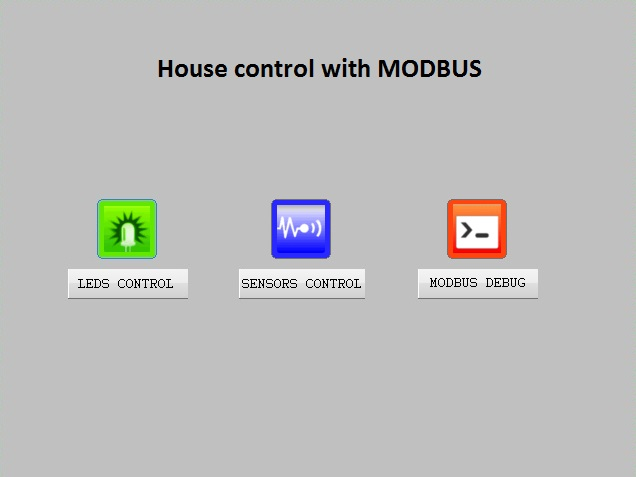
\includegraphics[scale=0.6]{menu.jpg}
\end{figure}

Il menù principale è composto da un titolo e da 3 bottoni; a questi bottoni è stata applicata un'icona intuitiva corrispondente alle funzionalità che devono eseguire.

Il primo bottone, la cui icona è un led verde, sottotitolato dalla label ``LEDS CONTROL'', avvia l'applicazione di controllo luci che si interfaccerà con il microcontrollore PIC16F77. Il secondo bottone, la cui icona è un sensore stilizzato bianco su sfondo blu, sottotitolato dalla label ``SENSORS ICON'', avvia l'applicazione di controllo sensori che comunicherà con il microprocessore LPC1768. Il terzo bottone, la cui icona è una riga di comando stilizzata con cornice arancione, sottotitolato dalla label ``MODBUS DEBUG'', avvia la schermata di debug, in cui si può interagire con tutti i dispositivi collegati al sistema.

~

In questa schermata tutti i controlli avvengono dall'interno dell'interfaccia, ovvero non esiste nessun task esterno che modifica l'interfaccia; quando viene eseguita un'applicazione, questa schermata si blocca e attende la sua chiusura prima di ripartire.

Bisogna notare che GUIBuilder non è in grado di applicare delle icone ai bottoni; per fare ciò, è stato necessario convertire le immagini presenti in un array di caratteri esadecimali e aggiungere questo array come icona del pulsante; il codice, per il bottone per l'applicazione del controllo luci, è il seguente:

\begin{lstlisting}

    //ottengo il puntatore al bottone
    hItem = WM_GetDialogItem(pMsg->hWin, ID_BUTTON_0);
    //cancello il testo dentro il bottone
    BUTTON_SetText( hItem, "");
    //imposto il colore di sfondo verde
    BUTTON_SetBkColor (hItem, 0, GUI_GREEN);
    //imposto il cambio colore al click giallo 
    BUTTON_SetBkColor (hItem, 1, GUI_YELLOW);
    //imposto l'immagine
    BUTTON_SetBitmapEx(hItem, 0, &bmled_icon, 5, 5);

\end{lstlisting} 

\newpage
\subsection{Controllo Luci}

\begin{figure}[!h]
\centering
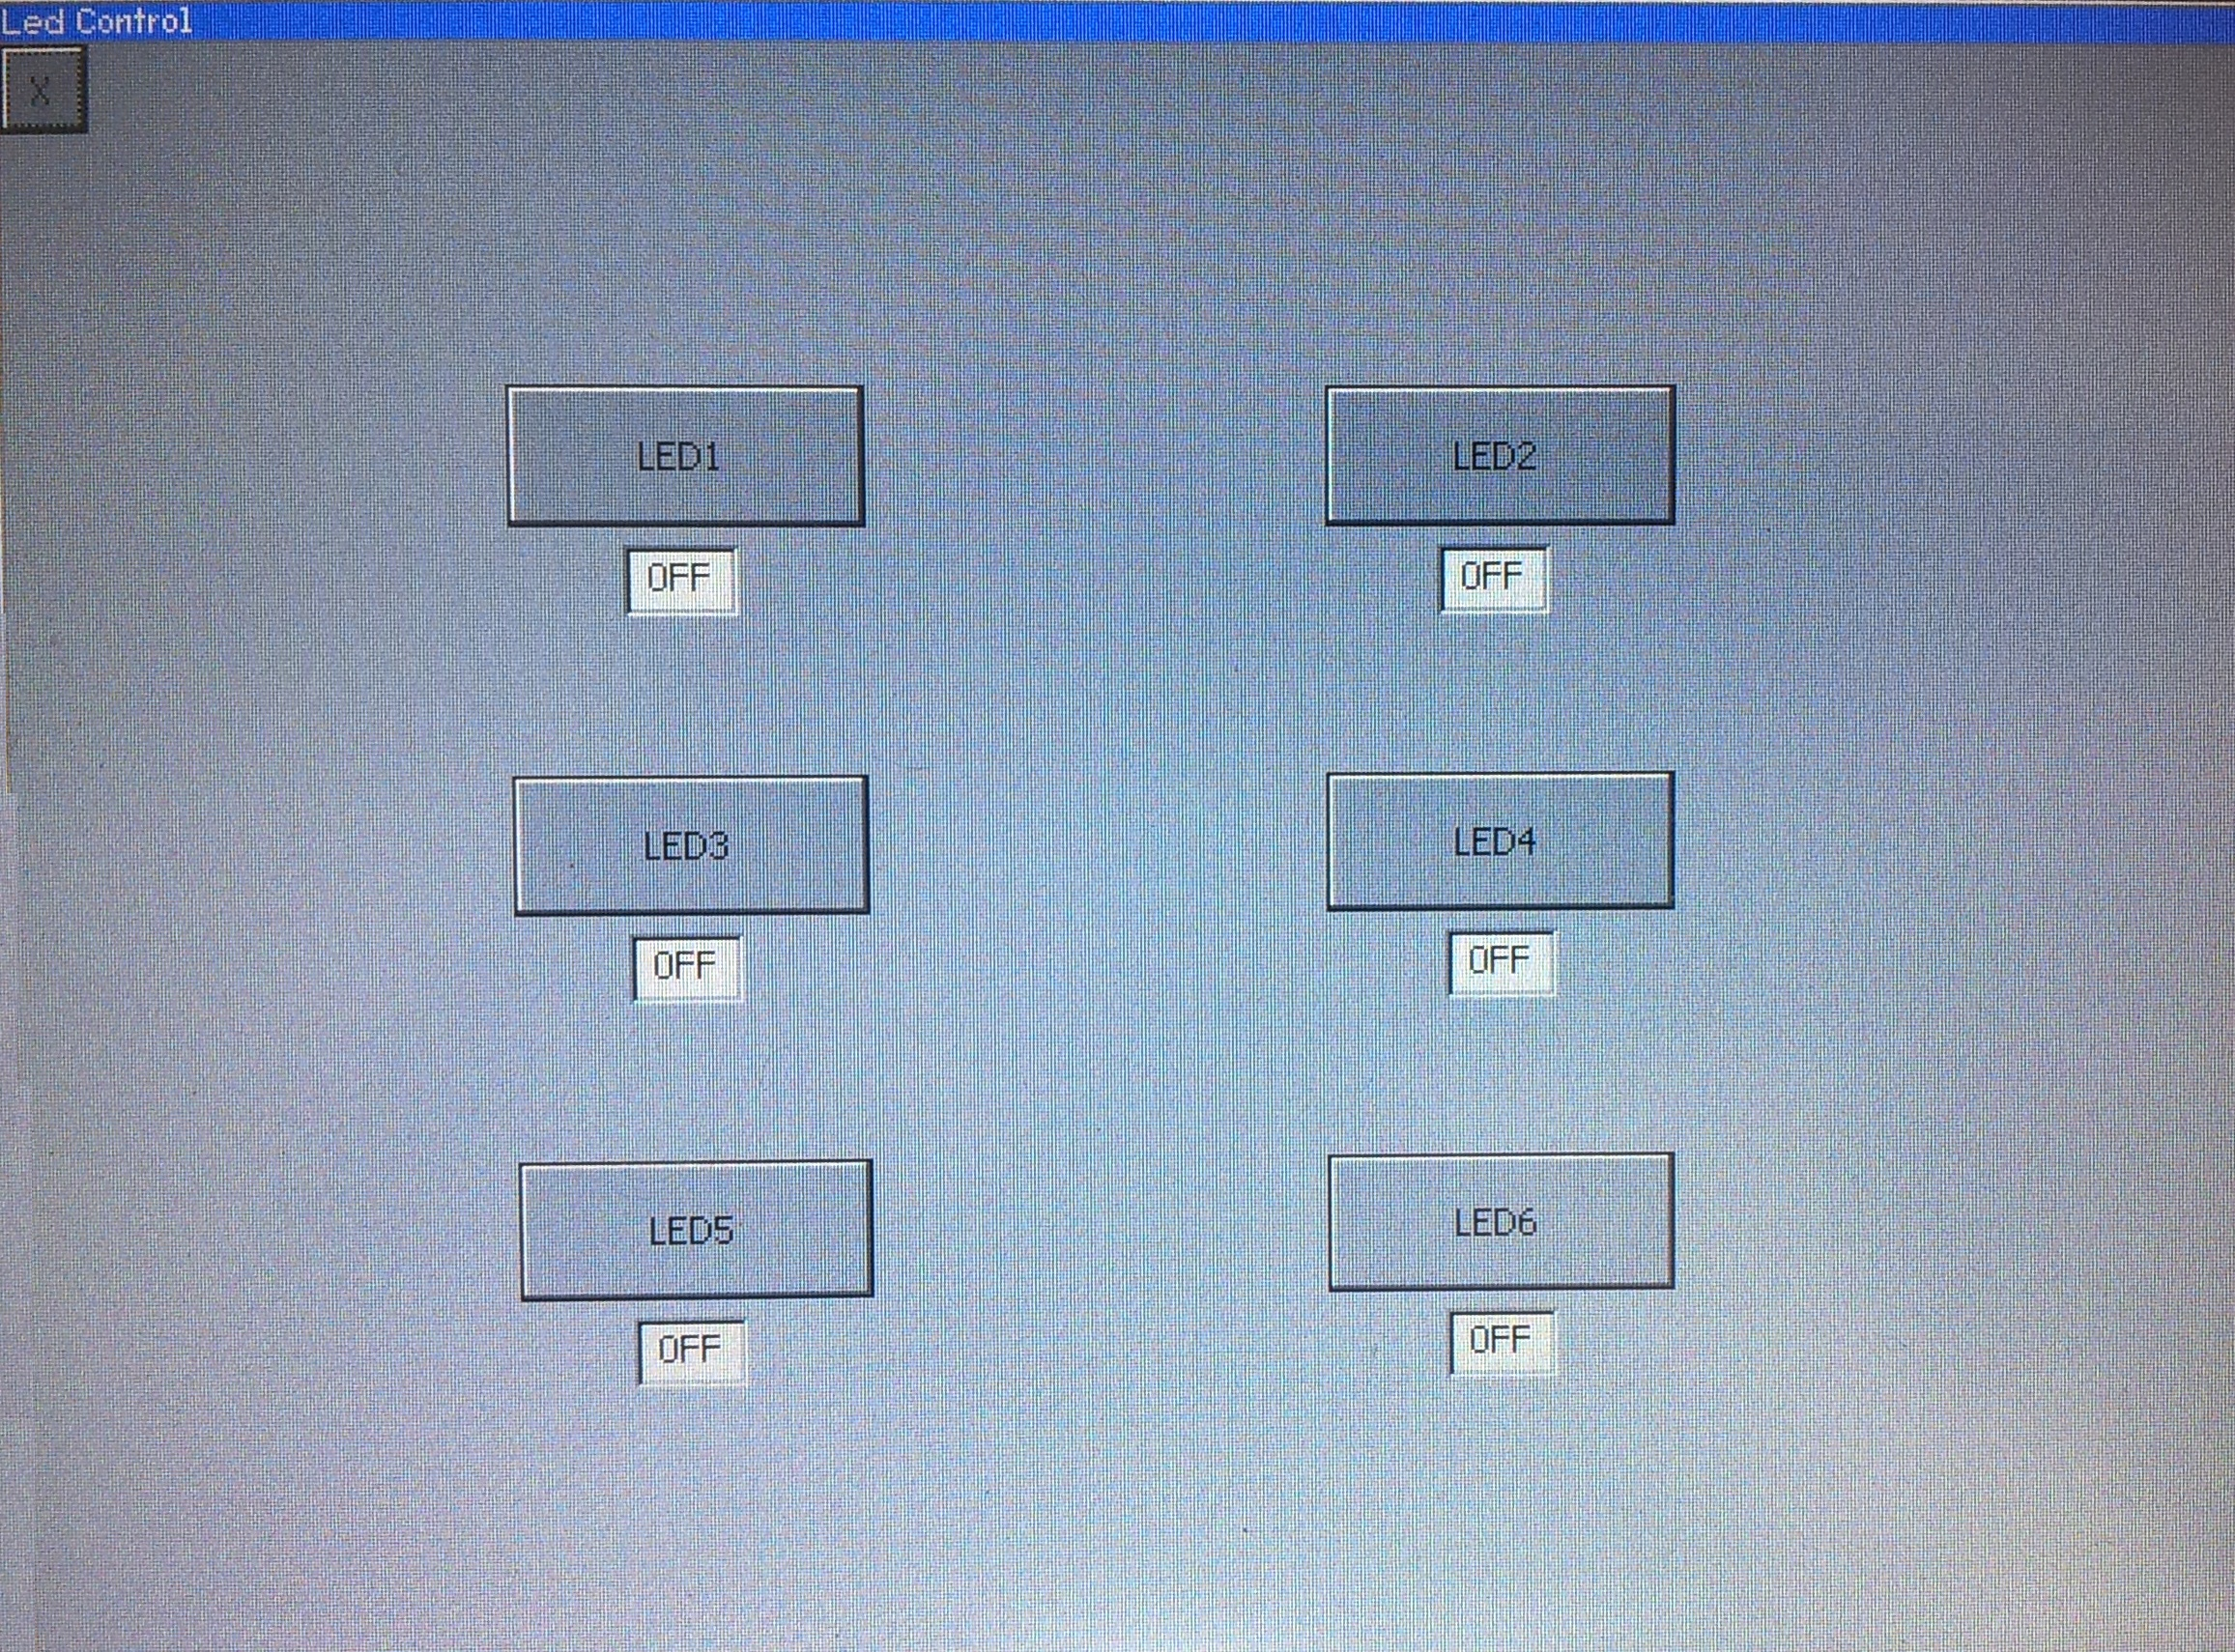
\includegraphics[scale=0.6]{ledgui.jpg}
\end{figure}

Questa schermata è composta da 6 bottoni che servono per inviare una richiesta di accensione o spegnimento del rispettivo led. Sotto ogni bottone è presente una sezione testuale in cui si scrive lo stato attuale del led (ON o OFF) e viene modificata dalla pressione dei tasti. Questa schermata si interfaccia esclusivamente con il microcontrollore PIC16F77 che ha lo slave id posto a 1. Per terminare l'esecuzione di questa applicazione, basta semplicemente premere il pulsante in alto a sinistra su cui è posta una ``X''.

~

Al momento dell'avvio di questa applicazione, viene inviata una richiesta al microcontrollore per sapere lo stato attuale delle luci, quindi, sapendo che le luci sono associate ai registri di coil, si farà una richiesta di tutti questi registri al microcontrollore; il risultato ottenuto verrà impostato sia sulla zona testuale sotto i bottoni sia alle variabili associate ai bottoni, in modo che, alla pressione dei pulsanti si invii la corretta richiesta (di accensione o spegnimento luci).

~

Durante l'esecuzione di questa applicazione, viene avviato un task asincrono che esegue continue richieste allo slave per sapere lo stato attuale delle luci; questo è molto utile se avviene un guasto momentaneo al microcontrollore (uno spegnimento improvviso), poiché verrà segnalato impostando ad OFF lo stato di tutte le luci (poiché verranno spente). Esiste quindi un task che modifica dall'esterno l'interfaccia grafica, quindi è possibile notare un cambiamento dell'interfaccia anche se non c'è stata alcuna interazione da parte dell'utente.


\newpage
\subsection{Controllo Sensori}

\begin{figure}[!h]
\centering
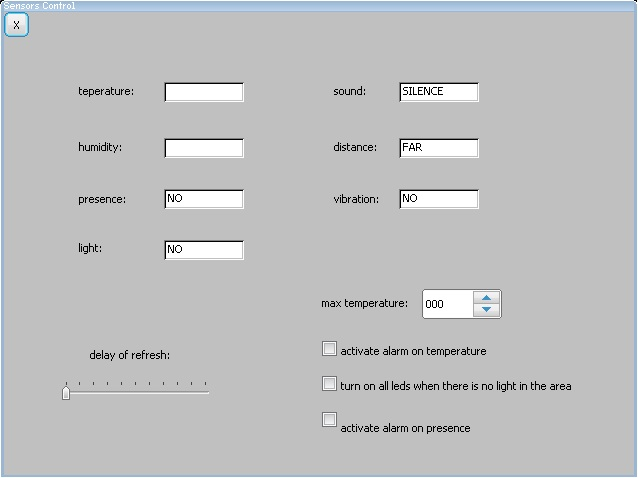
\includegraphics[scale=0.6]{sensorgui.jpg}
\end{figure}

Questa schermata è composta da 7 sezioni testuali associate ai vari controlli di sensori (a sinistra di ognuna è presente la descrizione), da uno spinbox che indica la temperatura limite da raggiungere prima di attivare l'allarme, da uno slider che modifica il delay di aggiornamento dello stato dei sensori e 3 checkbox che attivano o disattivano diverse funzionalità.

~

Al momento dell'avvio dell'applicazione, viene inviato un messaggio per richiedere lo stato dei sensori, in modo da inizializzare subito tutta la schermata. Questo è reso possibile da un task asincrono che viene creato al momento dell'avvio dell'applicazione e continua ad inviare richieste di aggiornamento di stato dei sensori al microprocessore LPC1768. Il ritardo del continuo invio richieste è modificabile dallo slider presente in basso a sinistra; questo ha un effetto particolare sul controllo della temperatura, in quanto più tardi si chiede lo stato attuale del sensore e più sarà preciso.

~

I tre checkbox attivano diverse funzionalità che mostrano l'applicazione effettiva di alcuni sensori:

\itema

\item il primo attiva un allarme sonoro al momento del raggiungimento della temperatura scelta, ossia attiva una specie di funzionalità termostato, utile per avvertire un utente quando fa troppo caldo o troppo freddo;

\item il secondo fa accendere tutte le luci quando non c'è abbastanza luce nella stanza, utile come interruttore crepuscolare per la notte;

\item il terzo attiva un allarme sonoro quando è presente un oggetto o una persona vicino al sensore presenza, utile per una funzione di antifurto.

\end{itemize}

Per uscire dall'applicazione, basta premere il bottone in alto a sinistra.

\newpage
\subsection{Schermata di Debug}

\begin{figure}[!h]
\centering
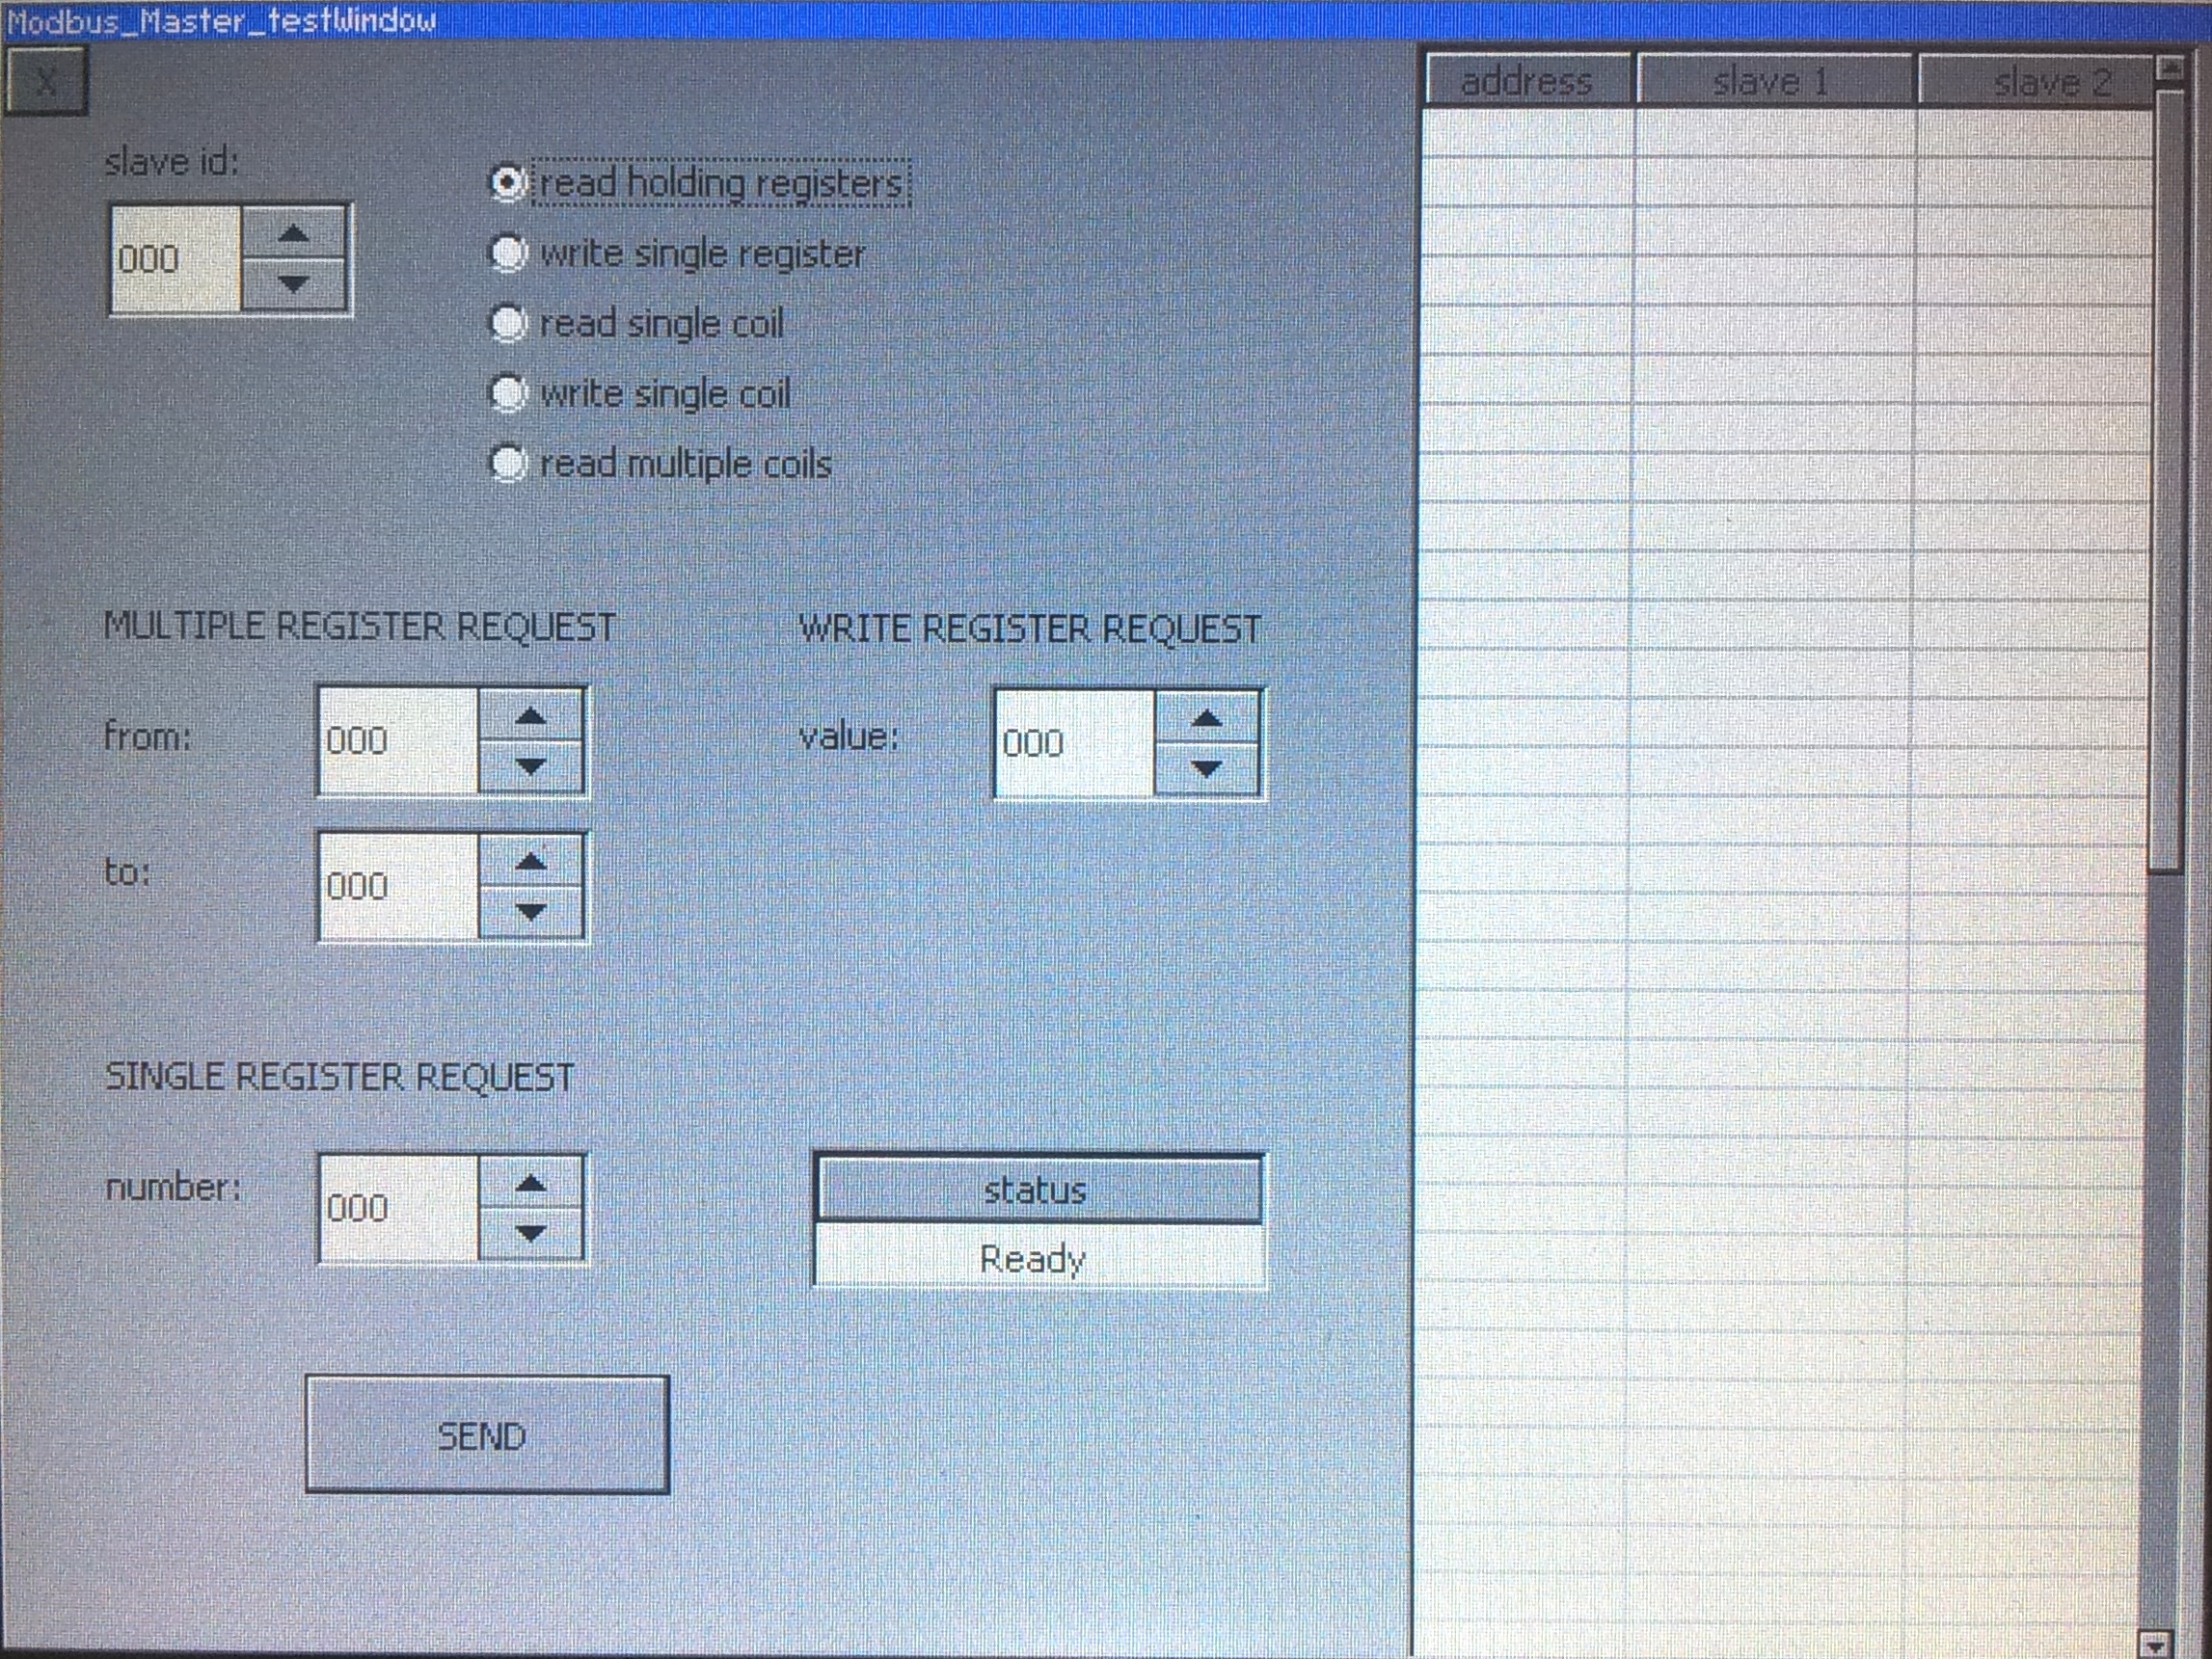
\includegraphics[scale=0.6]{debug.jpg}
\end{figure}

Questa è la parte applicativa più complessa dal punto di vista implementativo e ha l'esclusiva funzione di diagnostica di tutto il sistema: tramite questa, si è in grado di stabilire l'origine di un guasto o l'eventuale allacciamento di un nuovo Slave di controllo.

Sono presenti 5 spinbox, con cui si possono scegliere:

\itema

\item id dello Slave da interrogare;

\item l'indirizzo iniziale dei registri richiesti;

\item la quantità di registri richiesti;

\item l'indirizzo del singolo registro richiesto;

\item il valore da inserire in un regstro.

\end{itemize}

Poi è presente una selezione multipla tramite radio button, tramite cui si può scegliere la funzione Modbus da eseguire, quindi la rispettiva richiesta di registri. È presente anche una tabella laterale in cui vengono presentati i registri richiesti e il loro valore, in base alla richiesta eseguita. Inoltre è stata aggiunta una sezione testuale un basso a destra per descrivere l'esito della risposta: 

\itema

\item se lo Slave ha risposto correttamente alla richiesta, verrà scritto ``R: Message Accepted'' su sfondo verde;
\item se risponde con un CRC errato o si invia una richiesta senza senso per lo Slave (registri fuori dal suo range) verrà scritto ``R: Wrong Message'' su sfondo giallo;
\item se non si riceve risposta, verrà scritto ``No Response'' su sfondo rosso.

\end{itemize}

Infine è presente un bottone in basso per inviare la richiesta precedentemente composta allo Slave: quando viene premuto, viene inviata una richiesta Modbus; se lo Slave non risponde, viene inviata una seconda risposta con un minimo ritardo, se non risponde ancora viene segnalata la mancata risposta. Dopo la risposta, viene controllato il CRC e il codice funzione: se uno dei due risulta errato, viene segnalato come descritto precedentemente, altrimenti si procede con la conversione dei valori ottenuti e si aggiorna la schermata con i nuovi valori.

~

I valori ottenuti dall'interazione con la schermata vengono memorizzati nella struttura dati chiamata \code!GUI_value! che viene resettata al momento della chiusura di questa applicazione.

Per dedurre un potenziale guasto, si deve eseguire questo controllo:

\itema

\item se lo Slave non risponde, bisogna controllare il collegamento seriale, se il collegamento seriale è corretto, significa che lo Slave non funziona più correttamente;

\item se lo Slave invia una risposta non corretta, bisogna controllare lo stato del filo o se sono presenti dei disturbi tra il Master e lo Slave;

\item se lo Slave funziona e quindi invia una risposta corretta ma i sensori o le luci non cambiano stato in base agli stimoli, significa che questi non funzionano più correttamente.

\end{itemize}

\section{Interazione con i componenti hardware}

È stato deciso di dividere la gestione delle componenti hardware come segue.

\subsection{Sensori}

I sensori vengono pilotati e controllati dal processore LPC1768, in quanto offre un'interfaccia semplice per la gestione di questi componenti, oltrechè offre più sicurezza di controllo di questi. Infatti, avendo un sistema operativo, si è in grado di gestire il controllo dei sensori su threads diverse, in modo che non si sprechino risorse e che quindi il processore non riesca a gestire la parte più importante di tutto il sistema, ossia la comunicazione.

~

Per questo motivo questo slave è in grado di interpretare messaggi sia di lettura/scrittura di registri di holding, sia di registri di coil. I registri di holding verranno utilizzati per memorizzare ed inviare i valori ottenuti dal sensore di temperatura e di umidità, mentre i registri di coil per i sensori di vibrazione, di luce, di distanza e di ostacolo.

\subsection{Relè e luci}

I relè, e quindi anche le luci a led, vengono pilotati tramite il microcontrollore PIC16F77, in quanto non è in grado di eseguire operazioni troppo onerose (controllare in polling dei sensori non darebbe la possibilità di comunicare via Modbus) e offre un'interfaccia semplice di invio segnali digitali ai relè. Quando verrà attivato il segnale da parte del PIC, i relè verranno percorsi da corrente, creando quindi il contatto necessario per far ricevere corrente alle luci.

~

Per questo, lo slave è in grado di interpretare solo messaggi di lettura/scrittura coil, poiché rappresentano bene il messaggio di on/off dei relè. Nell'architettura di origine di questo protocollo infatti i registri di coil venivano associati direttamente ai relè collegati al PLC. 


\chapter{Diagramma dei componenti}

Di seguito si riporta l'organizzazione di tutto il progetto

\subsection{Architettura Hardware}

\begin{figure}[!h]
\centering
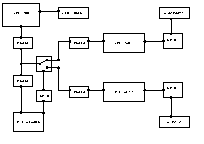
\includegraphics[scale=4.5]{archihard.pdf}
\caption{Architettura del sistema hardware}
\end{figure}

\newpage
\subsection{Architettura Software}
\begin{figure}[!h]
\centering
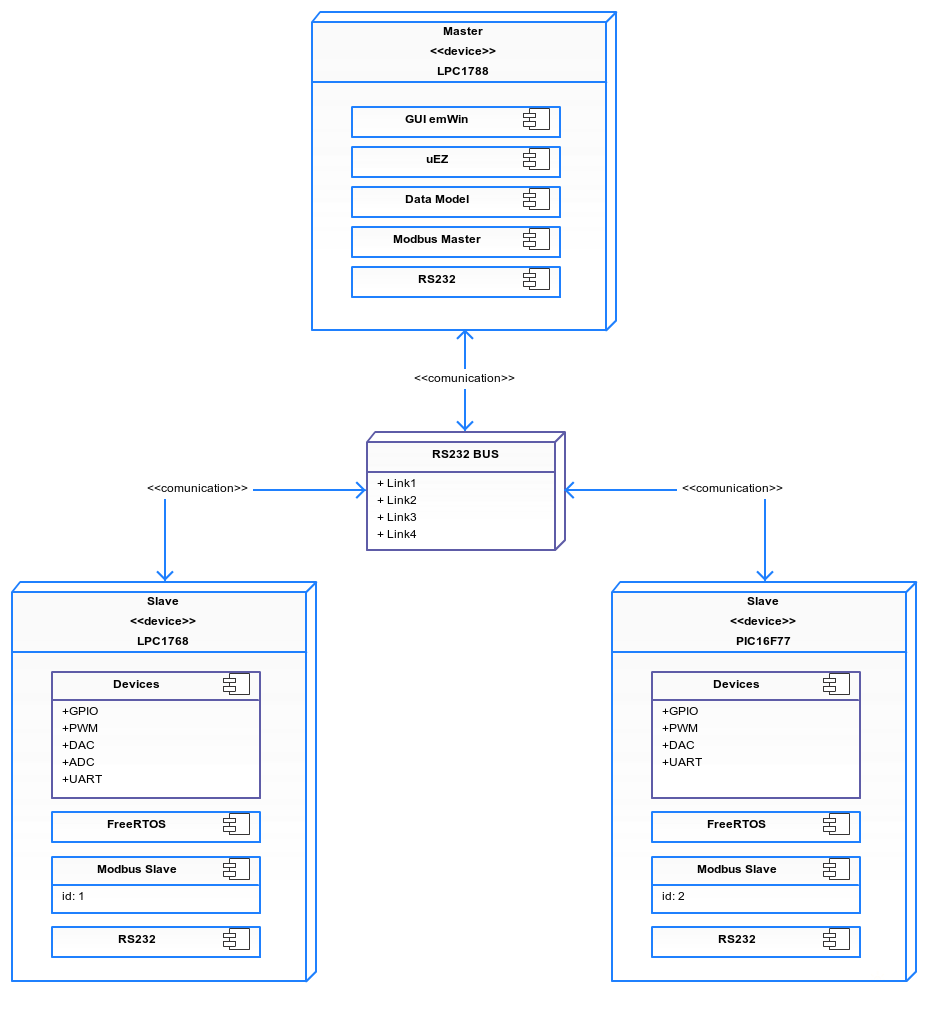
\includegraphics[scale=0.4]{deploy.png}
\caption{Architettura del sistema software}

\end{figure}


\chapter{Programmi utilizzati}

Poichè questo sistema richiedeva un notevole sforzo di progettazione, è stato deciso di usare degli IDE di sviluppo che rendessero più controllata la programmazione; ogni microprocessore è stato poi programmato con tecniche e strumenti differenti che ora verranno descritte. 

\section{LPC1788}

Poiché i sorgenti di $\mu EZ$ sono molti, i produttori di questo software hanno deciso di creare dei file di progetto in modo da rendere possibile l'apertura, la modifica e la ricompilazione dell'intero progetto a qualunque utente; perciò hanno creato dei file di progetto per Crossworks 2.1, Keil 4 e IAR 6.1. Di questi è stato scelto l'ambiente Keil, in quanto Crossworks, presente anche in Linux, doveva essere utilizzato esclusivamente in quella versione, ma ormai è stata rimossa dal mercato, e IAR non offriva una semplice interfaccia con il deploy su LPC1788.

Per rendere effettivamente funzionante la compilazione del progetto, sono state eseguite alcune modifiche sui sorgenti, oltre ad eliminare le funzioni ``printf'' in quanto non erano compatibili con la demoboard utilizzata.

~

Per la parte di deploy, è stato utilizzato il programmatore \textit{JLink Lite} di tipo JTAG presente nella scatola della demoboard. Per utilizzarlo, ci sono 2 opzioni:

\itema

\item tramite \textit{OpenOCD}, programma opensource i cui sorgenti di configurazione sono stati riscritti ad hoc per questo processore durante la progettazione (vedere file ``openocd2.cfg'');

\item tramite driver proprietari su Windows.

\end{itemize}

È stata scelta la seconda opzione in quanto, rendendo noti questi driver a Keil, è possibile fare deploy e debug all'interno dell'IDE, senza programmi aggiuntivi. Questa scelta ha notevolmente facilitato la progettazione.

\section{LPC1768}

In questa situazione, in cui non erano presenti sorgenti già pronti, la scelta dell'IDE è stata all'inizio casuale, in quanto questo microprocessore è piuttosto comune e si può programmare per esso con vari compilatori, tra cui \textit{gcc}. A seguito però della scelta dell'utilizzo di FreeRTOS e di alcuni vincoli sulla scelta delle librerie standard C per ARM compatibili per FreeModbus, è stato deciso di utilizzare LPCXpresso. Questo IDE, basato su Eclipse, offre la possibilità di creare un progetto basato su FreeRTOS e di cambiare le librerie standard da RedLib a NewLib (sono state utilizzate le NewLib); questo è reso possibile dal suo compilatore specifico.

~

Per la parte di deploy, poiché LPCXpresso non permette di interfacciarsi direttamente con il JTAG utilizzato, cioè ARM-USB-OCD, è stato utilizzato OpenOCD i cui file di configurazione sono stati riscritti per questo processore (vedere file ``openocd.cfg''), a cui si interfaccia il debugger specifico ARM chiamato ``arm-none-eabi-gdb''.

\section{PIC16F77}

Questa architettura è completamente diversa da quelle descritte precedentemente, in quanto i Pic non hanno la possibilità di comunicare via JTAG e fare il relativo deploy e debug, ma hanno bisogno di un hardware specifico. Per questo è stato utilizzato un programmatore specifico per Pic chiamato Pickit3, che esegue solamente il deploy attivando dei pin specifici del microcontrollore.

~

Per utilizzare il Pickit3 e compilare il progetto, è necessario utilizzare un IDE apposito chiamato MPLAB. Questo IDE però non offre il compilatore specifico per le famiglie di Pic, poiché bisognerebbe acquistarli. È stato quindi utilizzato un compilatore in versione Lite (non a pagamento ma non offre l'ottimizzazione massima di codice) chiamato XC8. 

\end{document}

